\documentclass[twoside]{book}

% Packages required by doxygen
\usepackage{calc}
\usepackage{doxygen}
\usepackage{graphicx}
\usepackage[utf8]{inputenc}
\usepackage{makeidx}
\usepackage{multicol}
\usepackage{multirow}
\usepackage{textcomp}
\usepackage[table]{xcolor}

% Font selection
\usepackage[T1]{fontenc}
\usepackage{mathptmx}
\usepackage[scaled=.90]{helvet}
\usepackage{courier}
\usepackage{amssymb}
\usepackage{sectsty}
\renewcommand{\familydefault}{\sfdefault}
\allsectionsfont{%
  \fontseries{bc}\selectfont%
  \color{darkgray}%
}
\renewcommand{\DoxyLabelFont}{%
  \fontseries{bc}\selectfont%
  \color{darkgray}%
}

% Page & text layout
\usepackage{geometry}
\geometry{%
  a4paper,%
  top=2.5cm,%
  bottom=2.5cm,%
  left=2.5cm,%
  right=2.5cm%
}
\tolerance=750
\hfuzz=15pt
\hbadness=750
\setlength{\emergencystretch}{15pt}
\setlength{\parindent}{0cm}
\setlength{\parskip}{0.2cm}
\makeatletter
\renewcommand{\paragraph}{%
  \@startsection{paragraph}{4}{0ex}{-1.0ex}{1.0ex}{%
    \normalfont\normalsize\bfseries\SS@parafont%
  }%
}
\renewcommand{\subparagraph}{%
  \@startsection{subparagraph}{5}{0ex}{-1.0ex}{1.0ex}{%
    \normalfont\normalsize\bfseries\SS@subparafont%
  }%
}
\makeatother

% Headers & footers
\usepackage{fancyhdr}
\pagestyle{fancyplain}
\fancyhead[LE]{\fancyplain{}{\bfseries\thepage}}
\fancyhead[CE]{\fancyplain{}{}}
\fancyhead[RE]{\fancyplain{}{\bfseries\leftmark}}
\fancyhead[LO]{\fancyplain{}{\bfseries\rightmark}}
\fancyhead[CO]{\fancyplain{}{}}
\fancyhead[RO]{\fancyplain{}{\bfseries\thepage}}
\fancyfoot[LE]{\fancyplain{}{}}
\fancyfoot[CE]{\fancyplain{}{}}
\fancyfoot[RE]{\fancyplain{}{\bfseries\scriptsize Generated on Mon May 4 2015 16\-:52\-:54 for Canbot\-Project\-Team\-D(2014-\/2015) by Doxygen }}
\fancyfoot[LO]{\fancyplain{}{\bfseries\scriptsize Generated on Mon May 4 2015 16\-:52\-:54 for Canbot\-Project\-Team\-D(2014-\/2015) by Doxygen }}
\fancyfoot[CO]{\fancyplain{}{}}
\fancyfoot[RO]{\fancyplain{}{}}
\renewcommand{\footrulewidth}{0.4pt}
\renewcommand{\chaptermark}[1]{%
  \markboth{#1}{}%
}
\renewcommand{\sectionmark}[1]{%
  \markright{\thesection\ #1}%
}

% Indices & bibliography
\usepackage{natbib}
\usepackage[titles]{tocloft}
\setcounter{tocdepth}{3}
\setcounter{secnumdepth}{5}
\makeindex

% Hyperlinks (required, but should be loaded last)
\usepackage{ifpdf}
\ifpdf
  \usepackage[pdftex,pagebackref=true]{hyperref}
\else
  \usepackage[ps2pdf,pagebackref=true]{hyperref}
\fi
\hypersetup{%
  colorlinks=true,%
  linkcolor=blue,%
  citecolor=blue,%
  unicode%
}

% Custom commands
\newcommand{\clearemptydoublepage}{%
  \newpage{\pagestyle{empty}\cleardoublepage}%
}


%===== C O N T E N T S =====

\begin{document}

% Titlepage & ToC
\hypersetup{pageanchor=false}
\pagenumbering{roman}
\begin{titlepage}
\vspace*{7cm}
\begin{center}%
{\Large Canbot\-Project\-Team\-D(2014-\/2015) \\[1ex]\large 1.\-1.\-1 }\\
\vspace*{1cm}
{\large Generated by Doxygen 1.8.6}\\
\vspace*{0.5cm}
{\small Mon May 4 2015 16:52:54}\\
\end{center}
\end{titlepage}
\clearemptydoublepage
\tableofcontents
\clearemptydoublepage
\pagenumbering{arabic}
\hypersetup{pageanchor=true}

%--- Begin generated contents ---
\chapter{Hierarchical Index}
\section{Class Hierarchy}
This inheritance list is sorted roughly, but not completely, alphabetically\-:\begin{DoxyCompactList}
\item \contentsline{section}{Average}{\pageref{classAverage}}{}
\item \contentsline{section}{Hoek}{\pageref{classHoek}}{}
\begin{DoxyCompactList}
\item \contentsline{section}{Robot}{\pageref{classRobot}}{}
\end{DoxyCompactList}
\item \contentsline{section}{Info}{\pageref{structInfo}}{}
\item \contentsline{section}{Package}{\pageref{structPackage}}{}
\item \contentsline{section}{Positie}{\pageref{classPositie}}{}
\item \contentsline{section}{robotcommand}{\pageref{classrobotcommand}}{}
\begin{DoxyCompactList}
\item \contentsline{section}{Robot}{\pageref{classRobot}}{}
\end{DoxyCompactList}
\item \contentsline{section}{serialport}{\pageref{classserialport}}{}
\item \contentsline{section}{Server}{\pageref{classServer}}{}
\begin{DoxyCompactList}
\item \contentsline{section}{Robot}{\pageref{classRobot}}{}
\end{DoxyCompactList}
\item \contentsline{section}{Udp\-\_\-header}{\pageref{structUdp__header}}{}
\item \contentsline{section}{Udp\-\_\-package}{\pageref{structUdp__package}}{}
\end{DoxyCompactList}

\chapter{Class Index}
\section{Class List}
Here are the classes, structs, unions and interfaces with brief descriptions\-:\begin{DoxyCompactList}
\item\contentsline{section}{\hyperlink{classAverage}{Average} }{\pageref{classAverage}}{}
\item\contentsline{section}{\hyperlink{classHoek}{Hoek} }{\pageref{classHoek}}{}
\item\contentsline{section}{\hyperlink{structInfo}{Info} }{\pageref{structInfo}}{}
\item\contentsline{section}{\hyperlink{structPackage}{Package} }{\pageref{structPackage}}{}
\item\contentsline{section}{\hyperlink{classPositie}{Positie} }{\pageref{classPositie}}{}
\item\contentsline{section}{\hyperlink{classRobot}{Robot} }{\pageref{classRobot}}{}
\item\contentsline{section}{\hyperlink{classrobotcommand}{robotcommand} }{\pageref{classrobotcommand}}{}
\item\contentsline{section}{\hyperlink{classserialport}{serialport} }{\pageref{classserialport}}{}
\item\contentsline{section}{\hyperlink{classServer}{Server} }{\pageref{classServer}}{}
\item\contentsline{section}{\hyperlink{structUdp__header}{Udp\-\_\-header} }{\pageref{structUdp__header}}{}
\item\contentsline{section}{\hyperlink{structUdp__package}{Udp\-\_\-package} }{\pageref{structUdp__package}}{}
\end{DoxyCompactList}

\chapter{File Index}
\section{File List}
Here is a list of all files with brief descriptions\-:\begin{DoxyCompactList}
\item\contentsline{section}{include/\hyperlink{Average_8h}{Average.\-h} }{\pageref{Average_8h}}{}
\item\contentsline{section}{include/\hyperlink{debug_8h}{debug.\-h} }{\pageref{debug_8h}}{}
\item\contentsline{section}{include/\hyperlink{Hoek_8h}{Hoek.\-h} }{\pageref{Hoek_8h}}{}
\item\contentsline{section}{include/\hyperlink{Package_8h}{Package.\-h} }{\pageref{Package_8h}}{}
\item\contentsline{section}{include/\hyperlink{Positie_8h}{Positie.\-h} }{\pageref{Positie_8h}}{}
\item\contentsline{section}{include/\hyperlink{Robot_8h}{Robot.\-h} }{\pageref{Robot_8h}}{}
\item\contentsline{section}{include/\hyperlink{robotcommand_8h}{robotcommand.\-h} }{\pageref{robotcommand_8h}}{}
\item\contentsline{section}{include/\hyperlink{serialport_8h}{serialport.\-h} }{\pageref{serialport_8h}}{}
\item\contentsline{section}{include/\hyperlink{Server_8h}{Server.\-h} }{\pageref{Server_8h}}{}
\item\contentsline{section}{src/\hyperlink{Average_8cpp}{Average.\-cpp} }{\pageref{Average_8cpp}}{}
\item\contentsline{section}{src/\hyperlink{Hoek_8cpp}{Hoek.\-cpp} }{\pageref{Hoek_8cpp}}{}
\item\contentsline{section}{src/\hyperlink{Positie_8cpp}{Positie.\-cpp} }{\pageref{Positie_8cpp}}{}
\item\contentsline{section}{src/\hyperlink{Robot_8cpp}{Robot.\-cpp} }{\pageref{Robot_8cpp}}{}
\item\contentsline{section}{src/\hyperlink{robotcommand_8cpp}{robotcommand.\-cpp} }{\pageref{robotcommand_8cpp}}{}
\item\contentsline{section}{src/\hyperlink{serialport_8cpp}{serialport.\-cpp} }{\pageref{serialport_8cpp}}{}
\item\contentsline{section}{src/\hyperlink{Server_8cpp}{Server.\-cpp} }{\pageref{Server_8cpp}}{}
\item\contentsline{section}{src/\hyperlink{udptest_8cpp}{udptest.\-cpp} }{\pageref{udptest_8cpp}}{}
\end{DoxyCompactList}

\chapter{Class Documentation}
\hypertarget{classAverage}{\section{Average Class Reference}
\label{classAverage}\index{Average@{Average}}
}


{\ttfamily \#include $<$Average.\-h$>$}



Collaboration diagram for Average\-:
\nopagebreak
\begin{figure}[H]
\begin{center}
\leavevmode
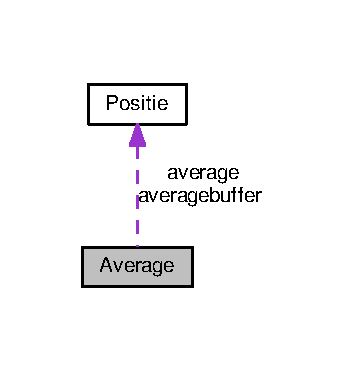
\includegraphics[width=166pt]{classAverage__coll__graph}
\end{center}
\end{figure}
\subsection*{Public Member Functions}
\begin{DoxyCompactItemize}
\item 
\hyperlink{classAverage_a25a54da41e8cae37098db4060ec5caf9}{Average} ()
\item 
int \hyperlink{classAverage_a0731ceab3cfbc6f88a26edc9319c778f}{get\-Nuber\-Samp} ()
\item 
\hyperlink{classPositie}{Positie} \hyperlink{classAverage_a80546f32249549643af4e09661763ec1}{get\-Average} ()
\item 
void \hyperlink{classAverage_a25f9ec5ac7f9f65e1d5af39b6d9626ec}{calc\-Average} ()
\item 
\hyperlink{classPositie}{Positie} \hyperlink{classAverage_a4e8e7238796949de80376e687f07dece}{get\-Calc\-Average} ()
\item 
\hyperlink{classPositie}{Positie} \hyperlink{classAverage_a607bf7034d4a7c3ef58f27b3cd7af943}{get\-Calc\-Average} (\hyperlink{classPositie}{Positie} val)
\item 
void \hyperlink{classAverage_a53554687cc447765fb0e9a7c3742fe89}{add\-Input\-Val} (\hyperlink{classPositie}{Positie} val)
\item 
void \hyperlink{classAverage_a954341c85ff2adf25f38e1769ec9d5cf}{print} ()
\end{DoxyCompactItemize}
\subsection*{Private Attributes}
\begin{DoxyCompactItemize}
\item 
\hyperlink{classPositie}{Positie} \hyperlink{classAverage_af3b416d3fd5e90e06467a37e9dcb86e1}{averagebuffer} \mbox{[}\hyperlink{Average_8h_a70d1b7be16e53d5ab19ecfe0d11c888f}{N\-U\-M\-S\-A\-M\-P\-L\-E\-S}\mbox{]}
\item 
\hyperlink{classPositie}{Positie} \hyperlink{classAverage_abcc8a32d2c44c97a84c10f5e093e6937}{average}
\item 
int \hyperlink{classAverage_acf70c3e32bfe44e11d20382f0015733e}{current\-Index}
\end{DoxyCompactItemize}


\subsection{Constructor \& Destructor Documentation}
\hypertarget{classAverage_a25a54da41e8cae37098db4060ec5caf9}{\index{Average@{Average}!Average@{Average}}
\index{Average@{Average}!Average@{Average}}
\subsubsection[{Average}]{\setlength{\rightskip}{0pt plus 5cm}Average\-::\-Average (
\begin{DoxyParamCaption}
{}
\end{DoxyParamCaption}
)}}\label{classAverage_a25a54da41e8cae37098db4060ec5caf9}


\subsection{Member Function Documentation}
\hypertarget{classAverage_a53554687cc447765fb0e9a7c3742fe89}{\index{Average@{Average}!add\-Input\-Val@{add\-Input\-Val}}
\index{add\-Input\-Val@{add\-Input\-Val}!Average@{Average}}
\subsubsection[{add\-Input\-Val}]{\setlength{\rightskip}{0pt plus 5cm}void Average\-::add\-Input\-Val (
\begin{DoxyParamCaption}
\item[{{\bf Positie}}]{val}
\end{DoxyParamCaption}
)}}\label{classAverage_a53554687cc447765fb0e9a7c3742fe89}
\hypertarget{classAverage_a25f9ec5ac7f9f65e1d5af39b6d9626ec}{\index{Average@{Average}!calc\-Average@{calc\-Average}}
\index{calc\-Average@{calc\-Average}!Average@{Average}}
\subsubsection[{calc\-Average}]{\setlength{\rightskip}{0pt plus 5cm}void Average\-::calc\-Average (
\begin{DoxyParamCaption}
{}
\end{DoxyParamCaption}
)}}\label{classAverage_a25f9ec5ac7f9f65e1d5af39b6d9626ec}


Here is the call graph for this function\-:
\nopagebreak
\begin{figure}[H]
\begin{center}
\leavevmode
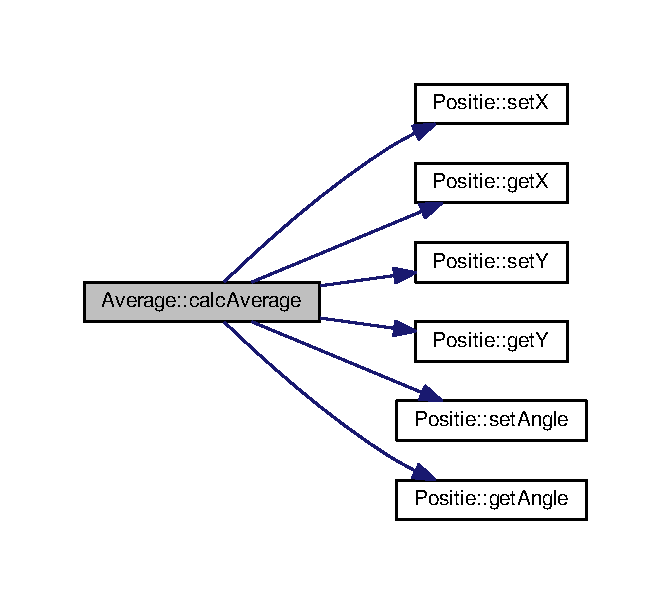
\includegraphics[width=322pt]{classAverage_a25f9ec5ac7f9f65e1d5af39b6d9626ec_cgraph}
\end{center}
\end{figure}


\hypertarget{classAverage_a80546f32249549643af4e09661763ec1}{\index{Average@{Average}!get\-Average@{get\-Average}}
\index{get\-Average@{get\-Average}!Average@{Average}}
\subsubsection[{get\-Average}]{\setlength{\rightskip}{0pt plus 5cm}{\bf Positie} Average\-::get\-Average (
\begin{DoxyParamCaption}
{}
\end{DoxyParamCaption}
)}}\label{classAverage_a80546f32249549643af4e09661763ec1}
\hypertarget{classAverage_a4e8e7238796949de80376e687f07dece}{\index{Average@{Average}!get\-Calc\-Average@{get\-Calc\-Average}}
\index{get\-Calc\-Average@{get\-Calc\-Average}!Average@{Average}}
\subsubsection[{get\-Calc\-Average}]{\setlength{\rightskip}{0pt plus 5cm}{\bf Positie} Average\-::get\-Calc\-Average (
\begin{DoxyParamCaption}
{}
\end{DoxyParamCaption}
)}}\label{classAverage_a4e8e7238796949de80376e687f07dece}


Here is the call graph for this function\-:
\nopagebreak
\begin{figure}[H]
\begin{center}
\leavevmode
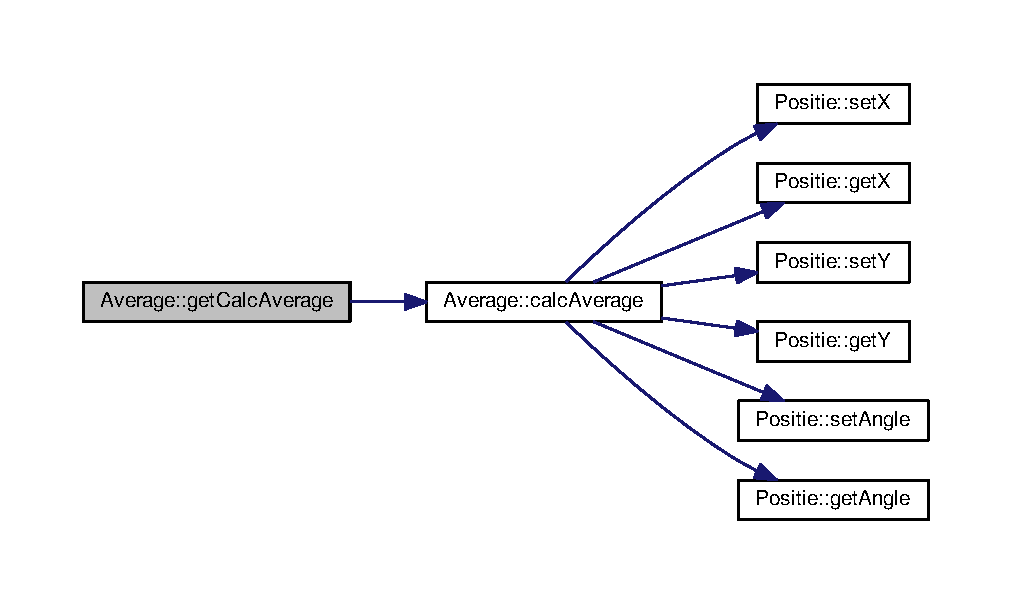
\includegraphics[width=350pt]{classAverage_a4e8e7238796949de80376e687f07dece_cgraph}
\end{center}
\end{figure}


\hypertarget{classAverage_a607bf7034d4a7c3ef58f27b3cd7af943}{\index{Average@{Average}!get\-Calc\-Average@{get\-Calc\-Average}}
\index{get\-Calc\-Average@{get\-Calc\-Average}!Average@{Average}}
\subsubsection[{get\-Calc\-Average}]{\setlength{\rightskip}{0pt plus 5cm}{\bf Positie} Average\-::get\-Calc\-Average (
\begin{DoxyParamCaption}
\item[{{\bf Positie}}]{val}
\end{DoxyParamCaption}
)}}\label{classAverage_a607bf7034d4a7c3ef58f27b3cd7af943}


Here is the call graph for this function\-:
\nopagebreak
\begin{figure}[H]
\begin{center}
\leavevmode
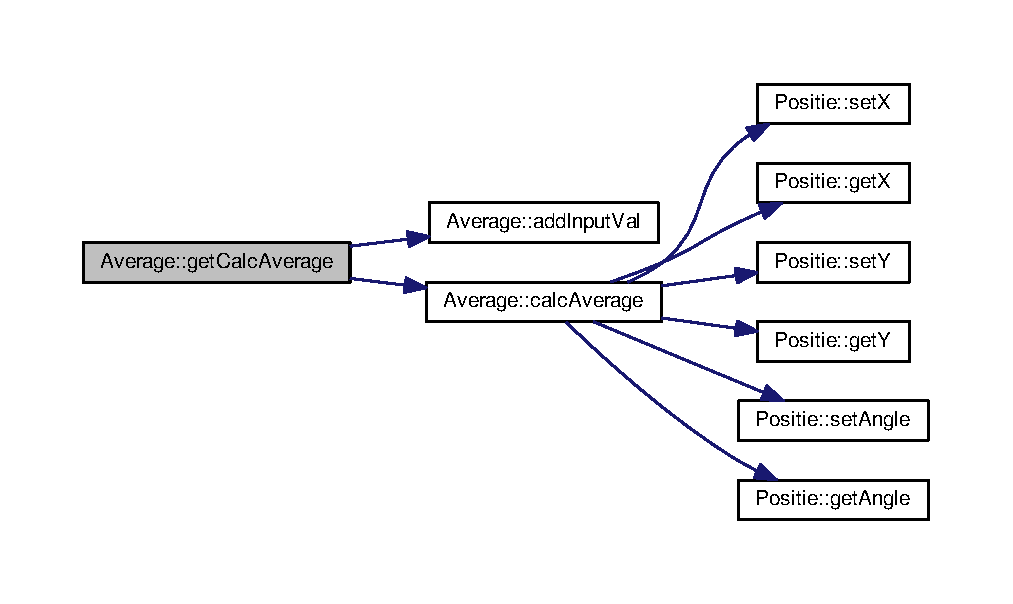
\includegraphics[width=350pt]{classAverage_a607bf7034d4a7c3ef58f27b3cd7af943_cgraph}
\end{center}
\end{figure}


\hypertarget{classAverage_a0731ceab3cfbc6f88a26edc9319c778f}{\index{Average@{Average}!get\-Nuber\-Samp@{get\-Nuber\-Samp}}
\index{get\-Nuber\-Samp@{get\-Nuber\-Samp}!Average@{Average}}
\subsubsection[{get\-Nuber\-Samp}]{\setlength{\rightskip}{0pt plus 5cm}int Average\-::get\-Nuber\-Samp (
\begin{DoxyParamCaption}
{}
\end{DoxyParamCaption}
)}}\label{classAverage_a0731ceab3cfbc6f88a26edc9319c778f}
\hypertarget{classAverage_a954341c85ff2adf25f38e1769ec9d5cf}{\index{Average@{Average}!print@{print}}
\index{print@{print}!Average@{Average}}
\subsubsection[{print}]{\setlength{\rightskip}{0pt plus 5cm}void Average\-::print (
\begin{DoxyParamCaption}
{}
\end{DoxyParamCaption}
)}}\label{classAverage_a954341c85ff2adf25f38e1769ec9d5cf}


Here is the call graph for this function\-:
\nopagebreak
\begin{figure}[H]
\begin{center}
\leavevmode
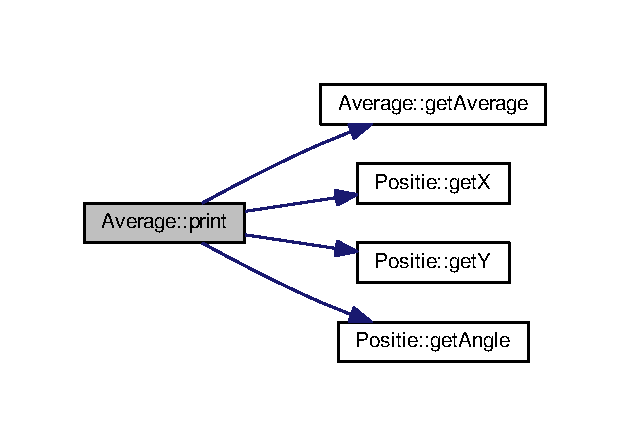
\includegraphics[width=302pt]{classAverage_a954341c85ff2adf25f38e1769ec9d5cf_cgraph}
\end{center}
\end{figure}




\subsection{Member Data Documentation}
\hypertarget{classAverage_abcc8a32d2c44c97a84c10f5e093e6937}{\index{Average@{Average}!average@{average}}
\index{average@{average}!Average@{Average}}
\subsubsection[{average}]{\setlength{\rightskip}{0pt plus 5cm}{\bf Positie} Average\-::average\hspace{0.3cm}{\ttfamily [private]}}}\label{classAverage_abcc8a32d2c44c97a84c10f5e093e6937}
\hypertarget{classAverage_af3b416d3fd5e90e06467a37e9dcb86e1}{\index{Average@{Average}!averagebuffer@{averagebuffer}}
\index{averagebuffer@{averagebuffer}!Average@{Average}}
\subsubsection[{averagebuffer}]{\setlength{\rightskip}{0pt plus 5cm}{\bf Positie} Average\-::averagebuffer\mbox{[}{\bf N\-U\-M\-S\-A\-M\-P\-L\-E\-S}\mbox{]}\hspace{0.3cm}{\ttfamily [private]}}}\label{classAverage_af3b416d3fd5e90e06467a37e9dcb86e1}
\hypertarget{classAverage_acf70c3e32bfe44e11d20382f0015733e}{\index{Average@{Average}!current\-Index@{current\-Index}}
\index{current\-Index@{current\-Index}!Average@{Average}}
\subsubsection[{current\-Index}]{\setlength{\rightskip}{0pt plus 5cm}int Average\-::current\-Index\hspace{0.3cm}{\ttfamily [private]}}}\label{classAverage_acf70c3e32bfe44e11d20382f0015733e}


The documentation for this class was generated from the following files\-:\begin{DoxyCompactItemize}
\item 
include/\hyperlink{Average_8h}{Average.\-h}\item 
src/\hyperlink{Average_8cpp}{Average.\-cpp}\end{DoxyCompactItemize}

\hypertarget{classHoek}{\section{Hoek Class Reference}
\label{classHoek}\index{Hoek@{Hoek}}
}


{\ttfamily \#include $<$Hoek.\-h$>$}



Inheritance diagram for Hoek\-:
\nopagebreak
\begin{figure}[H]
\begin{center}
\leavevmode
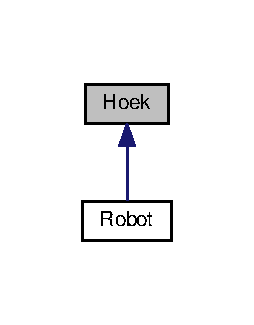
\includegraphics[width=122pt]{classHoek__inherit__graph}
\end{center}
\end{figure}
\subsection*{Public Member Functions}
\begin{DoxyCompactItemize}
\item 
\hyperlink{classHoek_a582c81967d4d5a0211faa32a9387457b}{$\sim$\-Hoek} ()
\item 
\hyperlink{classHoek_a00f72681885213e1d92bdd6d5e690081}{Hoek} ()
\item 
int \hyperlink{classHoek_a6418dc2139cedec6df600f7102ab4d95}{get\-Angle} ()
\item 
char \hyperlink{classHoek_af74f65686c7a2e9266853fa01dd74300}{get\-Direction} ()
\item 
int \hyperlink{classHoek_adefa1a4bc29befe4c2cee9026bed171b}{get\-Speed} ()
\item 
int \hyperlink{classHoek_a828b6cc7d878e741f463edc6f9d9253b}{get\-Afstand} ()
\item 
void \hyperlink{classHoek_a35ba5e42ed8ff1b5b95d568c46c4d7b0}{set\-Afstand} (int i\-\_\-\-Afstand)
\item 
void \hyperlink{classHoek_a810d85dd19ad702298481d8d596e40ae}{set\-Angle} (int Angle)
\item 
void \hyperlink{classHoek_a30c2341705ff4b57d662a47689a567bb}{set\-Direction} (char Direction)
\item 
void \hyperlink{classHoek_a3d3f8f53b047999c6da708df5128c2c8}{set\-Speed} (int Speed)
\item 
void \hyperlink{classHoek_a51fbe1b1eba5971727450d7880ab7422}{Bepaal\-Hoek} (int Xr, int Yr, int Xb, int Yb, int Beta)
\item 
void \hyperlink{classHoek_a03065000b2764ae9ad767bb22fde68f1}{Bepaal\-Snelheid} ()
\item 
void \hyperlink{classHoek_a7dab6f40d750f5e9d0c18ad8e1b75a91}{Bepaal\-Afstand} (int Xr, int Yr, int Xb, int Yb)
\end{DoxyCompactItemize}
\subsection*{Private Attributes}
\begin{DoxyCompactItemize}
\item 
int \hyperlink{classHoek_a7a64714ad3c3323e0db2a4efd254c6a2}{i\-\_\-\-Angle}
\item 
char \hyperlink{classHoek_a0ab8c37c98a7e3ed6d5b74013e9946ca}{c\-\_\-\-Direction}
\item 
int \hyperlink{classHoek_ad83215305ee0c803a4eedae37610cd9e}{i\-\_\-\-Speed}
\item 
int \hyperlink{classHoek_a007485bd11353762cc5f70f299729244}{i\-\_\-\-Distance}
\end{DoxyCompactItemize}


\subsection{Constructor \& Destructor Documentation}
\hypertarget{classHoek_a582c81967d4d5a0211faa32a9387457b}{\index{Hoek@{Hoek}!$\sim$\-Hoek@{$\sim$\-Hoek}}
\index{$\sim$\-Hoek@{$\sim$\-Hoek}!Hoek@{Hoek}}
\subsubsection[{$\sim$\-Hoek}]{\setlength{\rightskip}{0pt plus 5cm}Hoek\-::$\sim$\-Hoek (
\begin{DoxyParamCaption}
{}
\end{DoxyParamCaption}
)}}\label{classHoek_a582c81967d4d5a0211faa32a9387457b}
\hypertarget{classHoek_a00f72681885213e1d92bdd6d5e690081}{\index{Hoek@{Hoek}!Hoek@{Hoek}}
\index{Hoek@{Hoek}!Hoek@{Hoek}}
\subsubsection[{Hoek}]{\setlength{\rightskip}{0pt plus 5cm}Hoek\-::\-Hoek (
\begin{DoxyParamCaption}
{}
\end{DoxyParamCaption}
)}}\label{classHoek_a00f72681885213e1d92bdd6d5e690081}


\subsection{Member Function Documentation}
\hypertarget{classHoek_a7dab6f40d750f5e9d0c18ad8e1b75a91}{\index{Hoek@{Hoek}!Bepaal\-Afstand@{Bepaal\-Afstand}}
\index{Bepaal\-Afstand@{Bepaal\-Afstand}!Hoek@{Hoek}}
\subsubsection[{Bepaal\-Afstand}]{\setlength{\rightskip}{0pt plus 5cm}void Hoek\-::\-Bepaal\-Afstand (
\begin{DoxyParamCaption}
\item[{int}]{Xr, }
\item[{int}]{Yr, }
\item[{int}]{Xb, }
\item[{int}]{Yb}
\end{DoxyParamCaption}
)}}\label{classHoek_a7dab6f40d750f5e9d0c18ad8e1b75a91}
\hypertarget{classHoek_a51fbe1b1eba5971727450d7880ab7422}{\index{Hoek@{Hoek}!Bepaal\-Hoek@{Bepaal\-Hoek}}
\index{Bepaal\-Hoek@{Bepaal\-Hoek}!Hoek@{Hoek}}
\subsubsection[{Bepaal\-Hoek}]{\setlength{\rightskip}{0pt plus 5cm}void Hoek\-::\-Bepaal\-Hoek (
\begin{DoxyParamCaption}
\item[{int}]{Xr, }
\item[{int}]{Yr, }
\item[{int}]{Xb, }
\item[{int}]{Yb, }
\item[{int}]{Beta}
\end{DoxyParamCaption}
)}}\label{classHoek_a51fbe1b1eba5971727450d7880ab7422}
\hypertarget{classHoek_a03065000b2764ae9ad767bb22fde68f1}{\index{Hoek@{Hoek}!Bepaal\-Snelheid@{Bepaal\-Snelheid}}
\index{Bepaal\-Snelheid@{Bepaal\-Snelheid}!Hoek@{Hoek}}
\subsubsection[{Bepaal\-Snelheid}]{\setlength{\rightskip}{0pt plus 5cm}void Hoek\-::\-Bepaal\-Snelheid (
\begin{DoxyParamCaption}
{}
\end{DoxyParamCaption}
)}}\label{classHoek_a03065000b2764ae9ad767bb22fde68f1}
\hypertarget{classHoek_a828b6cc7d878e741f463edc6f9d9253b}{\index{Hoek@{Hoek}!get\-Afstand@{get\-Afstand}}
\index{get\-Afstand@{get\-Afstand}!Hoek@{Hoek}}
\subsubsection[{get\-Afstand}]{\setlength{\rightskip}{0pt plus 5cm}int Hoek\-::get\-Afstand (
\begin{DoxyParamCaption}
{}
\end{DoxyParamCaption}
)}}\label{classHoek_a828b6cc7d878e741f463edc6f9d9253b}
\hypertarget{classHoek_a6418dc2139cedec6df600f7102ab4d95}{\index{Hoek@{Hoek}!get\-Angle@{get\-Angle}}
\index{get\-Angle@{get\-Angle}!Hoek@{Hoek}}
\subsubsection[{get\-Angle}]{\setlength{\rightskip}{0pt plus 5cm}int Hoek\-::get\-Angle (
\begin{DoxyParamCaption}
{}
\end{DoxyParamCaption}
)}}\label{classHoek_a6418dc2139cedec6df600f7102ab4d95}
\hypertarget{classHoek_af74f65686c7a2e9266853fa01dd74300}{\index{Hoek@{Hoek}!get\-Direction@{get\-Direction}}
\index{get\-Direction@{get\-Direction}!Hoek@{Hoek}}
\subsubsection[{get\-Direction}]{\setlength{\rightskip}{0pt plus 5cm}char Hoek\-::get\-Direction (
\begin{DoxyParamCaption}
{}
\end{DoxyParamCaption}
)}}\label{classHoek_af74f65686c7a2e9266853fa01dd74300}
\hypertarget{classHoek_adefa1a4bc29befe4c2cee9026bed171b}{\index{Hoek@{Hoek}!get\-Speed@{get\-Speed}}
\index{get\-Speed@{get\-Speed}!Hoek@{Hoek}}
\subsubsection[{get\-Speed}]{\setlength{\rightskip}{0pt plus 5cm}int Hoek\-::get\-Speed (
\begin{DoxyParamCaption}
{}
\end{DoxyParamCaption}
)}}\label{classHoek_adefa1a4bc29befe4c2cee9026bed171b}
\hypertarget{classHoek_a35ba5e42ed8ff1b5b95d568c46c4d7b0}{\index{Hoek@{Hoek}!set\-Afstand@{set\-Afstand}}
\index{set\-Afstand@{set\-Afstand}!Hoek@{Hoek}}
\subsubsection[{set\-Afstand}]{\setlength{\rightskip}{0pt plus 5cm}void Hoek\-::set\-Afstand (
\begin{DoxyParamCaption}
\item[{int}]{i\-\_\-\-Afstand}
\end{DoxyParamCaption}
)}}\label{classHoek_a35ba5e42ed8ff1b5b95d568c46c4d7b0}
\hypertarget{classHoek_a810d85dd19ad702298481d8d596e40ae}{\index{Hoek@{Hoek}!set\-Angle@{set\-Angle}}
\index{set\-Angle@{set\-Angle}!Hoek@{Hoek}}
\subsubsection[{set\-Angle}]{\setlength{\rightskip}{0pt plus 5cm}void Hoek\-::set\-Angle (
\begin{DoxyParamCaption}
\item[{int}]{Angle}
\end{DoxyParamCaption}
)}}\label{classHoek_a810d85dd19ad702298481d8d596e40ae}
\hypertarget{classHoek_a30c2341705ff4b57d662a47689a567bb}{\index{Hoek@{Hoek}!set\-Direction@{set\-Direction}}
\index{set\-Direction@{set\-Direction}!Hoek@{Hoek}}
\subsubsection[{set\-Direction}]{\setlength{\rightskip}{0pt plus 5cm}void Hoek\-::set\-Direction (
\begin{DoxyParamCaption}
\item[{char}]{Direction}
\end{DoxyParamCaption}
)}}\label{classHoek_a30c2341705ff4b57d662a47689a567bb}
\hypertarget{classHoek_a3d3f8f53b047999c6da708df5128c2c8}{\index{Hoek@{Hoek}!set\-Speed@{set\-Speed}}
\index{set\-Speed@{set\-Speed}!Hoek@{Hoek}}
\subsubsection[{set\-Speed}]{\setlength{\rightskip}{0pt plus 5cm}void Hoek\-::set\-Speed (
\begin{DoxyParamCaption}
\item[{int}]{Speed}
\end{DoxyParamCaption}
)}}\label{classHoek_a3d3f8f53b047999c6da708df5128c2c8}


\subsection{Member Data Documentation}
\hypertarget{classHoek_a0ab8c37c98a7e3ed6d5b74013e9946ca}{\index{Hoek@{Hoek}!c\-\_\-\-Direction@{c\-\_\-\-Direction}}
\index{c\-\_\-\-Direction@{c\-\_\-\-Direction}!Hoek@{Hoek}}
\subsubsection[{c\-\_\-\-Direction}]{\setlength{\rightskip}{0pt plus 5cm}char Hoek\-::c\-\_\-\-Direction\hspace{0.3cm}{\ttfamily [private]}}}\label{classHoek_a0ab8c37c98a7e3ed6d5b74013e9946ca}
\hypertarget{classHoek_a7a64714ad3c3323e0db2a4efd254c6a2}{\index{Hoek@{Hoek}!i\-\_\-\-Angle@{i\-\_\-\-Angle}}
\index{i\-\_\-\-Angle@{i\-\_\-\-Angle}!Hoek@{Hoek}}
\subsubsection[{i\-\_\-\-Angle}]{\setlength{\rightskip}{0pt plus 5cm}int Hoek\-::i\-\_\-\-Angle\hspace{0.3cm}{\ttfamily [private]}}}\label{classHoek_a7a64714ad3c3323e0db2a4efd254c6a2}
\hypertarget{classHoek_a007485bd11353762cc5f70f299729244}{\index{Hoek@{Hoek}!i\-\_\-\-Distance@{i\-\_\-\-Distance}}
\index{i\-\_\-\-Distance@{i\-\_\-\-Distance}!Hoek@{Hoek}}
\subsubsection[{i\-\_\-\-Distance}]{\setlength{\rightskip}{0pt plus 5cm}int Hoek\-::i\-\_\-\-Distance\hspace{0.3cm}{\ttfamily [private]}}}\label{classHoek_a007485bd11353762cc5f70f299729244}
\hypertarget{classHoek_ad83215305ee0c803a4eedae37610cd9e}{\index{Hoek@{Hoek}!i\-\_\-\-Speed@{i\-\_\-\-Speed}}
\index{i\-\_\-\-Speed@{i\-\_\-\-Speed}!Hoek@{Hoek}}
\subsubsection[{i\-\_\-\-Speed}]{\setlength{\rightskip}{0pt plus 5cm}int Hoek\-::i\-\_\-\-Speed\hspace{0.3cm}{\ttfamily [private]}}}\label{classHoek_ad83215305ee0c803a4eedae37610cd9e}


The documentation for this class was generated from the following files\-:\begin{DoxyCompactItemize}
\item 
include/\hyperlink{Hoek_8h}{Hoek.\-h}\item 
src/\hyperlink{Hoek_8cpp}{Hoek.\-cpp}\end{DoxyCompactItemize}

\hypertarget{structInfo}{\section{Info Struct Reference}
\label{structInfo}\index{Info@{Info}}
}


{\ttfamily \#include $<$Package.\-h$>$}

\subsection*{Public Attributes}
\begin{DoxyCompactItemize}
\item 
int \hyperlink{structInfo_a61295f0c91f3af22416337bee785a9c2}{robotx}
\item 
int \hyperlink{structInfo_a2dacc6919a0cc7f80da3dc6db7588dd2}{roboty}
\item 
int \hyperlink{structInfo_a452cf47140c5cc9a2bdaf68012abb0dd}{robothoek}
\item 
int \hyperlink{structInfo_ab75b1c67a0eb23774acc62ee53e8d6a9}{blikx}
\item 
int \hyperlink{structInfo_a4abe3b1c4272e0596bd17630baf3eab6}{bliky}
\item 
int \hyperlink{structInfo_a3138ebfa6837af8a395731f1e1cd8f5a}{garagex}
\item 
int \hyperlink{structInfo_a8fffb2565daace7a478fb371d51d8d64}{garagey}
\end{DoxyCompactItemize}


\subsection{Member Data Documentation}
\hypertarget{structInfo_ab75b1c67a0eb23774acc62ee53e8d6a9}{\index{Info@{Info}!blikx@{blikx}}
\index{blikx@{blikx}!Info@{Info}}
\subsubsection[{blikx}]{\setlength{\rightskip}{0pt plus 5cm}int Info\-::blikx}}\label{structInfo_ab75b1c67a0eb23774acc62ee53e8d6a9}
\hypertarget{structInfo_a4abe3b1c4272e0596bd17630baf3eab6}{\index{Info@{Info}!bliky@{bliky}}
\index{bliky@{bliky}!Info@{Info}}
\subsubsection[{bliky}]{\setlength{\rightskip}{0pt plus 5cm}int Info\-::bliky}}\label{structInfo_a4abe3b1c4272e0596bd17630baf3eab6}
\hypertarget{structInfo_a3138ebfa6837af8a395731f1e1cd8f5a}{\index{Info@{Info}!garagex@{garagex}}
\index{garagex@{garagex}!Info@{Info}}
\subsubsection[{garagex}]{\setlength{\rightskip}{0pt plus 5cm}int Info\-::garagex}}\label{structInfo_a3138ebfa6837af8a395731f1e1cd8f5a}
\hypertarget{structInfo_a8fffb2565daace7a478fb371d51d8d64}{\index{Info@{Info}!garagey@{garagey}}
\index{garagey@{garagey}!Info@{Info}}
\subsubsection[{garagey}]{\setlength{\rightskip}{0pt plus 5cm}int Info\-::garagey}}\label{structInfo_a8fffb2565daace7a478fb371d51d8d64}
\hypertarget{structInfo_a452cf47140c5cc9a2bdaf68012abb0dd}{\index{Info@{Info}!robothoek@{robothoek}}
\index{robothoek@{robothoek}!Info@{Info}}
\subsubsection[{robothoek}]{\setlength{\rightskip}{0pt plus 5cm}int Info\-::robothoek}}\label{structInfo_a452cf47140c5cc9a2bdaf68012abb0dd}
\hypertarget{structInfo_a61295f0c91f3af22416337bee785a9c2}{\index{Info@{Info}!robotx@{robotx}}
\index{robotx@{robotx}!Info@{Info}}
\subsubsection[{robotx}]{\setlength{\rightskip}{0pt plus 5cm}int Info\-::robotx}}\label{structInfo_a61295f0c91f3af22416337bee785a9c2}
\hypertarget{structInfo_a2dacc6919a0cc7f80da3dc6db7588dd2}{\index{Info@{Info}!roboty@{roboty}}
\index{roboty@{roboty}!Info@{Info}}
\subsubsection[{roboty}]{\setlength{\rightskip}{0pt plus 5cm}int Info\-::roboty}}\label{structInfo_a2dacc6919a0cc7f80da3dc6db7588dd2}


The documentation for this struct was generated from the following file\-:\begin{DoxyCompactItemize}
\item 
include/\hyperlink{Package_8h}{Package.\-h}\end{DoxyCompactItemize}

\hypertarget{structPackage}{\section{Package Struct Reference}
\label{structPackage}\index{Package@{Package}}
}


{\ttfamily \#include $<$Package.\-h$>$}



Collaboration diagram for Package\-:
\nopagebreak
\begin{figure}[H]
\begin{center}
\leavevmode
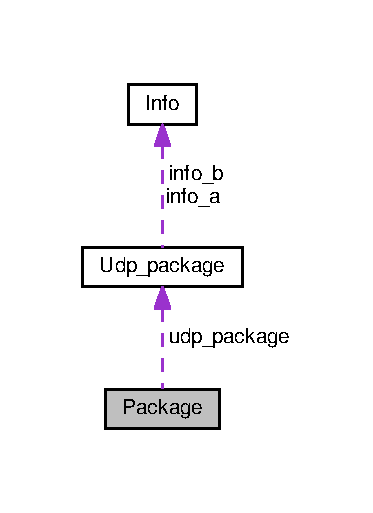
\includegraphics[width=179pt]{structPackage__coll__graph}
\end{center}
\end{figure}
\subsection*{Public Attributes}
\begin{DoxyCompactItemize}
\item 
int \hyperlink{structPackage_a562eb146b1c09eb1a819e2b36a64ecc3}{nr}
\item 
\hyperlink{structUdp__package}{Udp\-\_\-package} $\ast$ \hyperlink{structPackage_af73983d5bf7c911c68c9f74639d5f860}{udp\-\_\-package}
\end{DoxyCompactItemize}


\subsection{Member Data Documentation}
\hypertarget{structPackage_a562eb146b1c09eb1a819e2b36a64ecc3}{\index{Package@{Package}!nr@{nr}}
\index{nr@{nr}!Package@{Package}}
\subsubsection[{nr}]{\setlength{\rightskip}{0pt plus 5cm}int Package\-::nr}}\label{structPackage_a562eb146b1c09eb1a819e2b36a64ecc3}
\hypertarget{structPackage_af73983d5bf7c911c68c9f74639d5f860}{\index{Package@{Package}!udp\-\_\-package@{udp\-\_\-package}}
\index{udp\-\_\-package@{udp\-\_\-package}!Package@{Package}}
\subsubsection[{udp\-\_\-package}]{\setlength{\rightskip}{0pt plus 5cm}{\bf Udp\-\_\-package}$\ast$ Package\-::udp\-\_\-package}}\label{structPackage_af73983d5bf7c911c68c9f74639d5f860}


The documentation for this struct was generated from the following file\-:\begin{DoxyCompactItemize}
\item 
include/\hyperlink{Package_8h}{Package.\-h}\end{DoxyCompactItemize}

\hypertarget{classPositie}{\section{Positie Class Reference}
\label{classPositie}\index{Positie@{Positie}}
}


{\ttfamily \#include $<$Positie.\-h$>$}

\subsection*{Public Member Functions}
\begin{DoxyCompactItemize}
\item 
\hyperlink{classPositie_ab83d3eb64cbb064bd3aa8046b5ad5695}{Positie} ()
\item 
\hyperlink{classPositie_a32e5283bffdcfe28b28a27d0b2d04181}{Positie} (int new\-X, int new\-Y, int cor)
\item 
int \hyperlink{classPositie_a71dc2639feac7dc8d4f6f8a43bc7c98f}{get\-X} () const 
\item 
void \hyperlink{classPositie_a56f7076b52ce50e811ac5849f9631932}{set\-X} (int val)
\item 
int \hyperlink{classPositie_a42001a6907b4c6c360ffbf298923de75}{get\-Y} () const 
\item 
void \hyperlink{classPositie_ae230b789e2683561ac44f18162541da0}{set\-Y} (int val)
\item 
int \hyperlink{classPositie_a2b5bedcfc88cb380b8acb8dc27cb64e7}{get\-Angle} () const 
\item 
void \hyperlink{classPositie_ad6db714754c841515436dbbd73dc90ef}{set\-Angle} (int ang)
\item 
void \hyperlink{classPositie_a6ba64177362977ad0716ad9e06648799}{new\-Position} (int new\-X, int new\-Y, int cor)
\item 
bool \hyperlink{classPositie_adefdd66faaa3f410d5629a3affb88a47}{operator==} (const \hyperlink{classPositie}{Positie} \&rhs) const 
\item 
bool \hyperlink{classPositie_a320017884675a2c82af2bbcc7456e015}{operator!=} (const \hyperlink{classPositie}{Positie} \&rhs) const 
\item 
void \hyperlink{classPositie_a2124867ad0604af3aee6df0c1c9b438b}{print} ()
\end{DoxyCompactItemize}
\subsection*{Private Member Functions}
\begin{DoxyCompactItemize}
\item 
bool \hyperlink{classPositie_a38beabee21e6794fe6f7884f95fb5664}{helper\-Equal\-Operator} (const \hyperlink{classPositie}{Positie} \&rhs) const 
\end{DoxyCompactItemize}
\subsection*{Private Attributes}
\begin{DoxyCompactItemize}
\item 
int \hyperlink{classPositie_a008403bc70c73cd5e32922054dd41782}{x}
\item 
int \hyperlink{classPositie_a8eed2beb3e65dce35802a4b85936f497}{y}
\item 
int \hyperlink{classPositie_aa052314b6d640497b28f7c002b1ab424}{angle}
\end{DoxyCompactItemize}


\subsection{Constructor \& Destructor Documentation}
\hypertarget{classPositie_ab83d3eb64cbb064bd3aa8046b5ad5695}{\index{Positie@{Positie}!Positie@{Positie}}
\index{Positie@{Positie}!Positie@{Positie}}
\subsubsection[{Positie}]{\setlength{\rightskip}{0pt plus 5cm}Positie\-::\-Positie (
\begin{DoxyParamCaption}
{}
\end{DoxyParamCaption}
)}}\label{classPositie_ab83d3eb64cbb064bd3aa8046b5ad5695}


Here is the call graph for this function\-:
\nopagebreak
\begin{figure}[H]
\begin{center}
\leavevmode
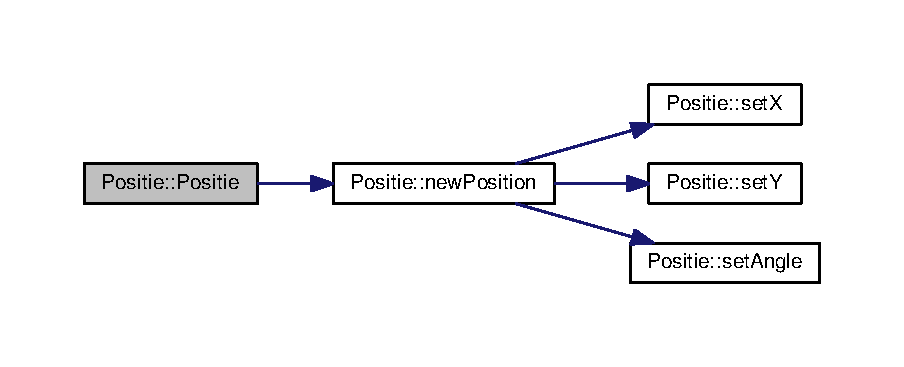
\includegraphics[width=350pt]{classPositie_ab83d3eb64cbb064bd3aa8046b5ad5695_cgraph}
\end{center}
\end{figure}


\hypertarget{classPositie_a32e5283bffdcfe28b28a27d0b2d04181}{\index{Positie@{Positie}!Positie@{Positie}}
\index{Positie@{Positie}!Positie@{Positie}}
\subsubsection[{Positie}]{\setlength{\rightskip}{0pt plus 5cm}Positie\-::\-Positie (
\begin{DoxyParamCaption}
\item[{int}]{new\-X, }
\item[{int}]{new\-Y, }
\item[{int}]{cor}
\end{DoxyParamCaption}
)}}\label{classPositie_a32e5283bffdcfe28b28a27d0b2d04181}


Here is the call graph for this function\-:
\nopagebreak
\begin{figure}[H]
\begin{center}
\leavevmode
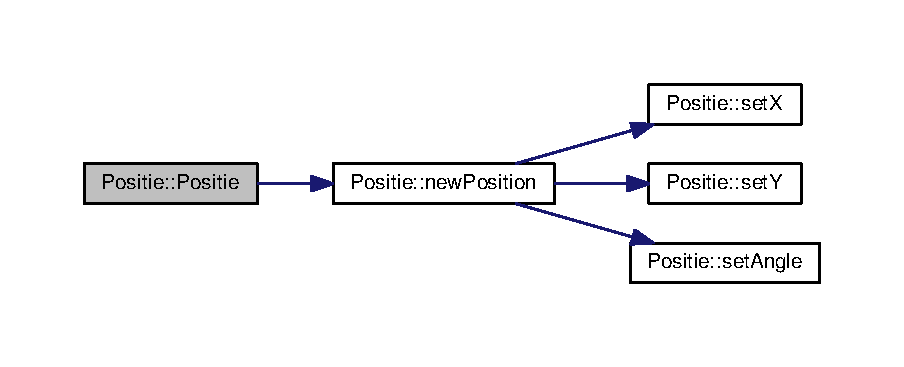
\includegraphics[width=350pt]{classPositie_a32e5283bffdcfe28b28a27d0b2d04181_cgraph}
\end{center}
\end{figure}




\subsection{Member Function Documentation}
\hypertarget{classPositie_a2b5bedcfc88cb380b8acb8dc27cb64e7}{\index{Positie@{Positie}!get\-Angle@{get\-Angle}}
\index{get\-Angle@{get\-Angle}!Positie@{Positie}}
\subsubsection[{get\-Angle}]{\setlength{\rightskip}{0pt plus 5cm}int Positie\-::get\-Angle (
\begin{DoxyParamCaption}
{}
\end{DoxyParamCaption}
) const}}\label{classPositie_a2b5bedcfc88cb380b8acb8dc27cb64e7}
\hypertarget{classPositie_a71dc2639feac7dc8d4f6f8a43bc7c98f}{\index{Positie@{Positie}!get\-X@{get\-X}}
\index{get\-X@{get\-X}!Positie@{Positie}}
\subsubsection[{get\-X}]{\setlength{\rightskip}{0pt plus 5cm}int Positie\-::get\-X (
\begin{DoxyParamCaption}
{}
\end{DoxyParamCaption}
) const}}\label{classPositie_a71dc2639feac7dc8d4f6f8a43bc7c98f}
\hypertarget{classPositie_a42001a6907b4c6c360ffbf298923de75}{\index{Positie@{Positie}!get\-Y@{get\-Y}}
\index{get\-Y@{get\-Y}!Positie@{Positie}}
\subsubsection[{get\-Y}]{\setlength{\rightskip}{0pt plus 5cm}int Positie\-::get\-Y (
\begin{DoxyParamCaption}
{}
\end{DoxyParamCaption}
) const}}\label{classPositie_a42001a6907b4c6c360ffbf298923de75}
\hypertarget{classPositie_a38beabee21e6794fe6f7884f95fb5664}{\index{Positie@{Positie}!helper\-Equal\-Operator@{helper\-Equal\-Operator}}
\index{helper\-Equal\-Operator@{helper\-Equal\-Operator}!Positie@{Positie}}
\subsubsection[{helper\-Equal\-Operator}]{\setlength{\rightskip}{0pt plus 5cm}bool Positie\-::helper\-Equal\-Operator (
\begin{DoxyParamCaption}
\item[{const {\bf Positie} \&}]{rhs}
\end{DoxyParamCaption}
) const\hspace{0.3cm}{\ttfamily [private]}}}\label{classPositie_a38beabee21e6794fe6f7884f95fb5664}


Here is the call graph for this function\-:
\nopagebreak
\begin{figure}[H]
\begin{center}
\leavevmode
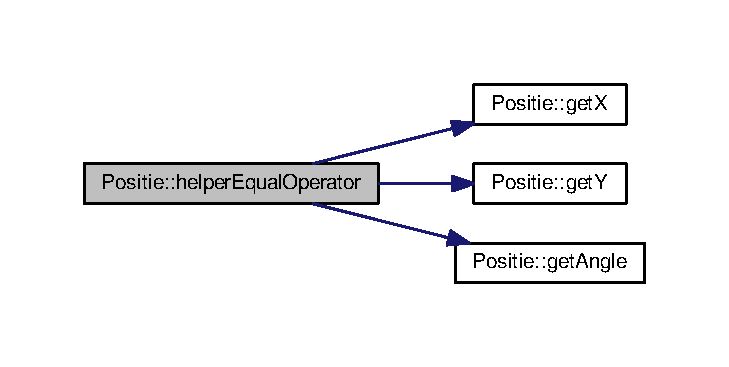
\includegraphics[width=350pt]{classPositie_a38beabee21e6794fe6f7884f95fb5664_cgraph}
\end{center}
\end{figure}


\hypertarget{classPositie_a6ba64177362977ad0716ad9e06648799}{\index{Positie@{Positie}!new\-Position@{new\-Position}}
\index{new\-Position@{new\-Position}!Positie@{Positie}}
\subsubsection[{new\-Position}]{\setlength{\rightskip}{0pt plus 5cm}void Positie\-::new\-Position (
\begin{DoxyParamCaption}
\item[{int}]{new\-X, }
\item[{int}]{new\-Y, }
\item[{int}]{cor}
\end{DoxyParamCaption}
)}}\label{classPositie_a6ba64177362977ad0716ad9e06648799}


Here is the call graph for this function\-:
\nopagebreak
\begin{figure}[H]
\begin{center}
\leavevmode
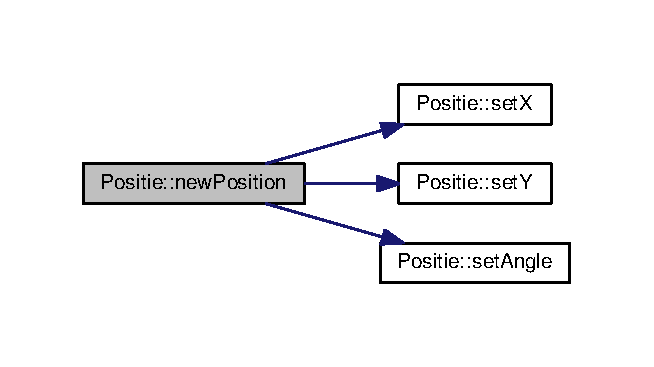
\includegraphics[width=314pt]{classPositie_a6ba64177362977ad0716ad9e06648799_cgraph}
\end{center}
\end{figure}


\hypertarget{classPositie_a320017884675a2c82af2bbcc7456e015}{\index{Positie@{Positie}!operator!=@{operator!=}}
\index{operator!=@{operator!=}!Positie@{Positie}}
\subsubsection[{operator!=}]{\setlength{\rightskip}{0pt plus 5cm}bool Positie\-::operator!= (
\begin{DoxyParamCaption}
\item[{const {\bf Positie} \&}]{rhs}
\end{DoxyParamCaption}
) const}}\label{classPositie_a320017884675a2c82af2bbcc7456e015}


Here is the call graph for this function\-:
\nopagebreak
\begin{figure}[H]
\begin{center}
\leavevmode
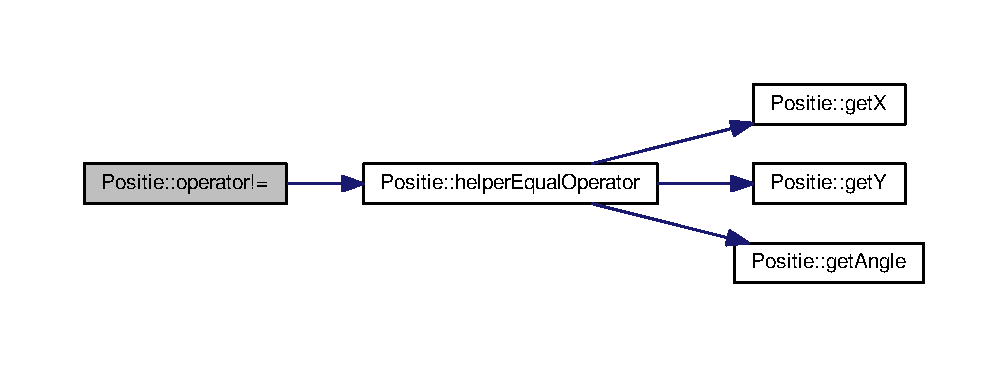
\includegraphics[width=350pt]{classPositie_a320017884675a2c82af2bbcc7456e015_cgraph}
\end{center}
\end{figure}


\hypertarget{classPositie_adefdd66faaa3f410d5629a3affb88a47}{\index{Positie@{Positie}!operator==@{operator==}}
\index{operator==@{operator==}!Positie@{Positie}}
\subsubsection[{operator==}]{\setlength{\rightskip}{0pt plus 5cm}bool Positie\-::operator== (
\begin{DoxyParamCaption}
\item[{const {\bf Positie} \&}]{rhs}
\end{DoxyParamCaption}
) const}}\label{classPositie_adefdd66faaa3f410d5629a3affb88a47}


Here is the call graph for this function\-:
\nopagebreak
\begin{figure}[H]
\begin{center}
\leavevmode
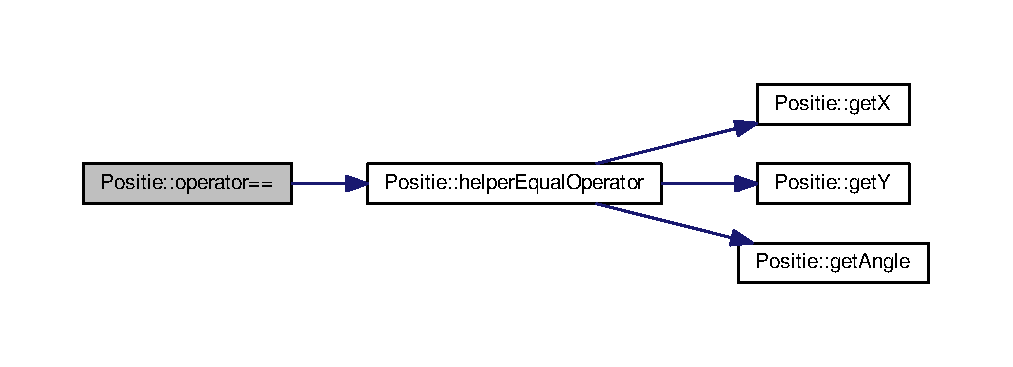
\includegraphics[width=350pt]{classPositie_adefdd66faaa3f410d5629a3affb88a47_cgraph}
\end{center}
\end{figure}


\hypertarget{classPositie_a2124867ad0604af3aee6df0c1c9b438b}{\index{Positie@{Positie}!print@{print}}
\index{print@{print}!Positie@{Positie}}
\subsubsection[{print}]{\setlength{\rightskip}{0pt plus 5cm}void Positie\-::print (
\begin{DoxyParamCaption}
{}
\end{DoxyParamCaption}
)}}\label{classPositie_a2124867ad0604af3aee6df0c1c9b438b}


Here is the call graph for this function\-:
\nopagebreak
\begin{figure}[H]
\begin{center}
\leavevmode
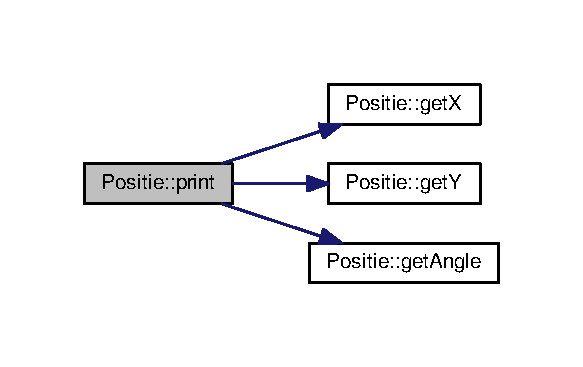
\includegraphics[width=280pt]{classPositie_a2124867ad0604af3aee6df0c1c9b438b_cgraph}
\end{center}
\end{figure}


\hypertarget{classPositie_ad6db714754c841515436dbbd73dc90ef}{\index{Positie@{Positie}!set\-Angle@{set\-Angle}}
\index{set\-Angle@{set\-Angle}!Positie@{Positie}}
\subsubsection[{set\-Angle}]{\setlength{\rightskip}{0pt plus 5cm}void Positie\-::set\-Angle (
\begin{DoxyParamCaption}
\item[{int}]{ang}
\end{DoxyParamCaption}
)}}\label{classPositie_ad6db714754c841515436dbbd73dc90ef}
\hypertarget{classPositie_a56f7076b52ce50e811ac5849f9631932}{\index{Positie@{Positie}!set\-X@{set\-X}}
\index{set\-X@{set\-X}!Positie@{Positie}}
\subsubsection[{set\-X}]{\setlength{\rightskip}{0pt plus 5cm}void Positie\-::set\-X (
\begin{DoxyParamCaption}
\item[{int}]{val}
\end{DoxyParamCaption}
)}}\label{classPositie_a56f7076b52ce50e811ac5849f9631932}
\hypertarget{classPositie_ae230b789e2683561ac44f18162541da0}{\index{Positie@{Positie}!set\-Y@{set\-Y}}
\index{set\-Y@{set\-Y}!Positie@{Positie}}
\subsubsection[{set\-Y}]{\setlength{\rightskip}{0pt plus 5cm}void Positie\-::set\-Y (
\begin{DoxyParamCaption}
\item[{int}]{val}
\end{DoxyParamCaption}
)}}\label{classPositie_ae230b789e2683561ac44f18162541da0}


\subsection{Member Data Documentation}
\hypertarget{classPositie_aa052314b6d640497b28f7c002b1ab424}{\index{Positie@{Positie}!angle@{angle}}
\index{angle@{angle}!Positie@{Positie}}
\subsubsection[{angle}]{\setlength{\rightskip}{0pt plus 5cm}int Positie\-::angle\hspace{0.3cm}{\ttfamily [private]}}}\label{classPositie_aa052314b6d640497b28f7c002b1ab424}
\hypertarget{classPositie_a008403bc70c73cd5e32922054dd41782}{\index{Positie@{Positie}!x@{x}}
\index{x@{x}!Positie@{Positie}}
\subsubsection[{x}]{\setlength{\rightskip}{0pt plus 5cm}int Positie\-::x\hspace{0.3cm}{\ttfamily [private]}}}\label{classPositie_a008403bc70c73cd5e32922054dd41782}
\hypertarget{classPositie_a8eed2beb3e65dce35802a4b85936f497}{\index{Positie@{Positie}!y@{y}}
\index{y@{y}!Positie@{Positie}}
\subsubsection[{y}]{\setlength{\rightskip}{0pt plus 5cm}int Positie\-::y\hspace{0.3cm}{\ttfamily [private]}}}\label{classPositie_a8eed2beb3e65dce35802a4b85936f497}


The documentation for this class was generated from the following files\-:\begin{DoxyCompactItemize}
\item 
include/\hyperlink{Positie_8h}{Positie.\-h}\item 
src/\hyperlink{Positie_8cpp}{Positie.\-cpp}\end{DoxyCompactItemize}

\hypertarget{classRobot}{\section{Robot Class Reference}
\label{classRobot}\index{Robot@{Robot}}
}


{\ttfamily \#include $<$Robot.\-h$>$}



Inheritance diagram for Robot\-:
\nopagebreak
\begin{figure}[H]
\begin{center}
\leavevmode
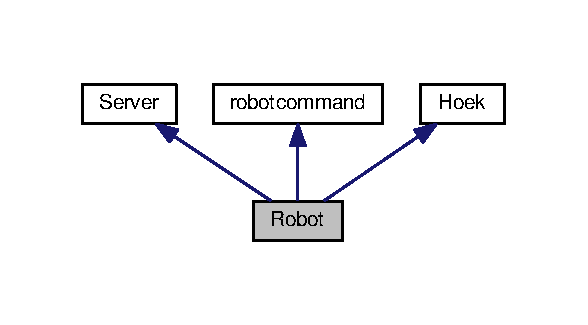
\includegraphics[width=282pt]{classRobot__inherit__graph}
\end{center}
\end{figure}


Collaboration diagram for Robot\-:
\nopagebreak
\begin{figure}[H]
\begin{center}
\leavevmode
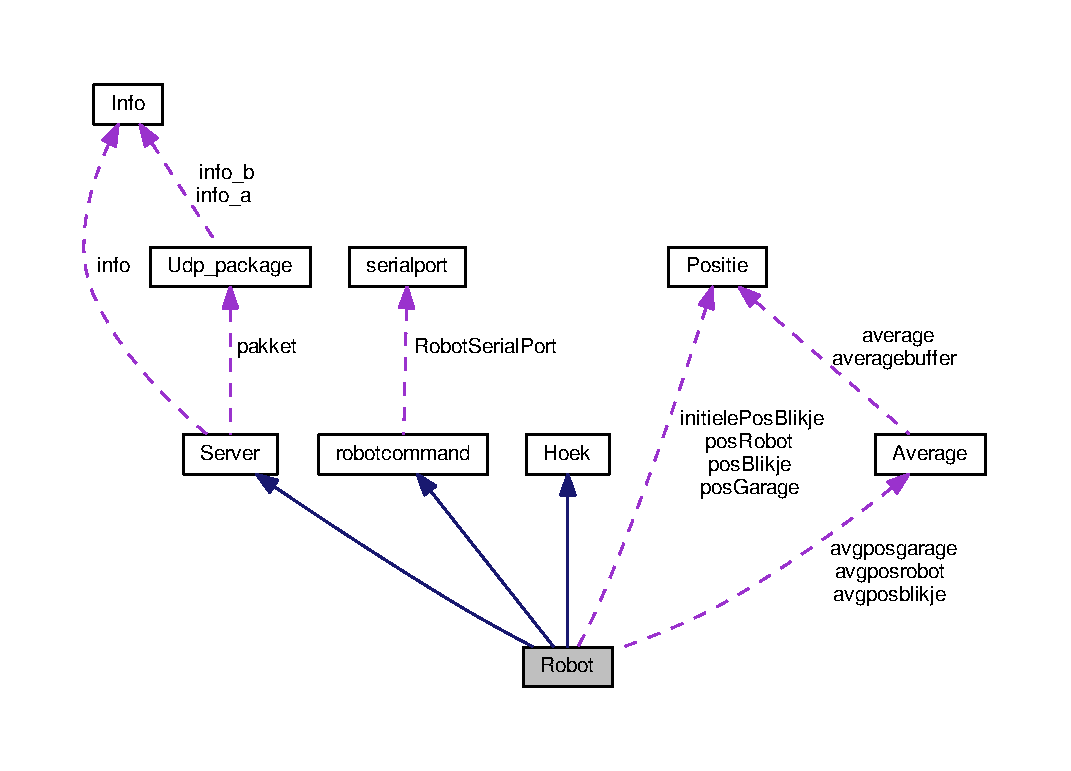
\includegraphics[width=350pt]{classRobot__coll__graph}
\end{center}
\end{figure}
\subsection*{Public Member Functions}
\begin{DoxyCompactItemize}
\item 
\hyperlink{classRobot_aa269489a0691f410fb286301be6d2434}{Robot} (int udp\-Poort, string serial\-Poort, char \hyperlink{classServer_ae63c2574fcde32ea16b06b0bcb61b716}{groep})
\item 
\hyperlink{classPositie}{Positie} \hyperlink{classRobot_a43fdd19ef403be762d659593023dda8a}{get\-Positie\-Robot} ()
\item 
void \hyperlink{classRobot_a6d3de1bc1f766693e4058a02a7744293}{set\-Positie\-Robot} (\hyperlink{classPositie}{Positie} val)
\item 
void \hyperlink{classRobot_a3f35253e8b6e3810aa377c9f3c4158de}{set\-Positie\-Robot} (int x, int y, int angle)
\item 
\hyperlink{classPositie}{Positie} \hyperlink{classRobot_abfab62ce2a3ff22f237e34ad1a6650e7}{get\-Positie\-Blikje} ()
\item 
void \hyperlink{classRobot_ad1c9b6e11cfb97e966350162ef38c7a2}{set\-Positie\-Blikje} (\hyperlink{classPositie}{Positie} val)
\item 
void \hyperlink{classRobot_a29185fbf1e17fe20b357afb1753bb29e}{set\-Positie\-Blikje} (int x, int y)
\item 
\hyperlink{classPositie}{Positie} \hyperlink{classRobot_a9301d035810174edffb769fd097f2a0c}{get\-Positie\-Garage} ()
\item 
void \hyperlink{classRobot_affb796dc23ca48799c1fc9ab31f578d9}{set\-Positie\-Garage} (\hyperlink{classPositie}{Positie} val)
\item 
void \hyperlink{classRobot_a371cff32d467a1cbaf2a8d212921845a}{set\-Positie\-Garage} (int x, int y)
\item 
void \hyperlink{classRobot_a17c05db895bbe8696acb2e0079f68de0}{set\-Initiele\-Pos\-Blikje\-Geset} (bool b)
\item 
void \hyperlink{classRobot_a4895306b538817f9044c1b9b69e89781}{print} ()
\item 
bool \hyperlink{classRobot_ab6fc311f9a66f524aac0757a7b2a4a57}{blikje\-Verplaatst} ()
\item 
void \hyperlink{classRobot_a980d1f972db40e5afcf3e2caf6ba346c}{update\-Posities} ()
\item 
void \hyperlink{classRobot_a1cbfcc8e3580c8ac369dc696dbdd640c}{bepaal\-Hoek\-Blikje} ()
\item 
void \hyperlink{classRobot_a5b40bae7bd0b458676caf2f5288d2047}{bepaal\-Hoek\-Garage} ()
\item 
void \hyperlink{classRobot_a80ce23f76438783761968602b801a401}{bepaal\-Afstand\-Blikje} ()
\item 
void \hyperlink{classRobot_a212f7383710351d161f084720aac00ad}{bepaal\-Afstand\-Garage} ()
\end{DoxyCompactItemize}
\subsection*{Private Attributes}
\begin{DoxyCompactItemize}
\item 
bool \hyperlink{classRobot_a89cba58927f6471cc51991ea6d1a5009}{initiele\-Pos\-Blikje\-Geset}
\item 
\hyperlink{classPositie}{Positie} \hyperlink{classRobot_a96f64e31d55c578095db9cd225597763}{initiele\-Pos\-Blikje}
\item 
\hyperlink{classPositie}{Positie} \hyperlink{classRobot_a9d4895475ce429baafb7056bba91892d}{pos\-Robot}
\item 
\hyperlink{classPositie}{Positie} \hyperlink{classRobot_a430b77999d3080962df243cc80ff41cc}{pos\-Blikje}
\item 
\hyperlink{classPositie}{Positie} \hyperlink{classRobot_a65d03adc264ed54988a63793bd1ee9c5}{pos\-Garage}
\item 
\hyperlink{classAverage}{Average} \hyperlink{classRobot_afb0e831757aefcfe83bd3df04d8ab4e7}{avgposrobot}
\item 
\hyperlink{classAverage}{Average} \hyperlink{classRobot_a6914cbc8706b7a2096b39a3a059b31bf}{avgposblikje}
\item 
\hyperlink{classAverage}{Average} \hyperlink{classRobot_ab74847d7cebe2e6141ec9ff00745594c}{avgposgarage}
\end{DoxyCompactItemize}


\subsection{Constructor \& Destructor Documentation}
\hypertarget{classRobot_aa269489a0691f410fb286301be6d2434}{\index{Robot@{Robot}!Robot@{Robot}}
\index{Robot@{Robot}!Robot@{Robot}}
\subsubsection[{Robot}]{\setlength{\rightskip}{0pt plus 5cm}Robot\-::\-Robot (
\begin{DoxyParamCaption}
\item[{int}]{udp\-Poort, }
\item[{string}]{serial\-Poort, }
\item[{char}]{groep}
\end{DoxyParamCaption}
)}}\label{classRobot_aa269489a0691f410fb286301be6d2434}


\subsection{Member Function Documentation}
\hypertarget{classRobot_a80ce23f76438783761968602b801a401}{\index{Robot@{Robot}!bepaal\-Afstand\-Blikje@{bepaal\-Afstand\-Blikje}}
\index{bepaal\-Afstand\-Blikje@{bepaal\-Afstand\-Blikje}!Robot@{Robot}}
\subsubsection[{bepaal\-Afstand\-Blikje}]{\setlength{\rightskip}{0pt plus 5cm}void Robot\-::bepaal\-Afstand\-Blikje (
\begin{DoxyParamCaption}
{}
\end{DoxyParamCaption}
)}}\label{classRobot_a80ce23f76438783761968602b801a401}


Here is the call graph for this function\-:
\nopagebreak
\begin{figure}[H]
\begin{center}
\leavevmode
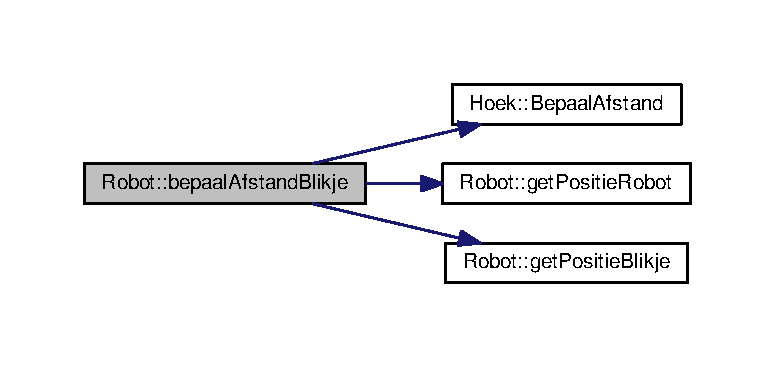
\includegraphics[width=350pt]{classRobot_a80ce23f76438783761968602b801a401_cgraph}
\end{center}
\end{figure}


\hypertarget{classRobot_a212f7383710351d161f084720aac00ad}{\index{Robot@{Robot}!bepaal\-Afstand\-Garage@{bepaal\-Afstand\-Garage}}
\index{bepaal\-Afstand\-Garage@{bepaal\-Afstand\-Garage}!Robot@{Robot}}
\subsubsection[{bepaal\-Afstand\-Garage}]{\setlength{\rightskip}{0pt plus 5cm}void Robot\-::bepaal\-Afstand\-Garage (
\begin{DoxyParamCaption}
{}
\end{DoxyParamCaption}
)}}\label{classRobot_a212f7383710351d161f084720aac00ad}


Here is the call graph for this function\-:
\nopagebreak
\begin{figure}[H]
\begin{center}
\leavevmode
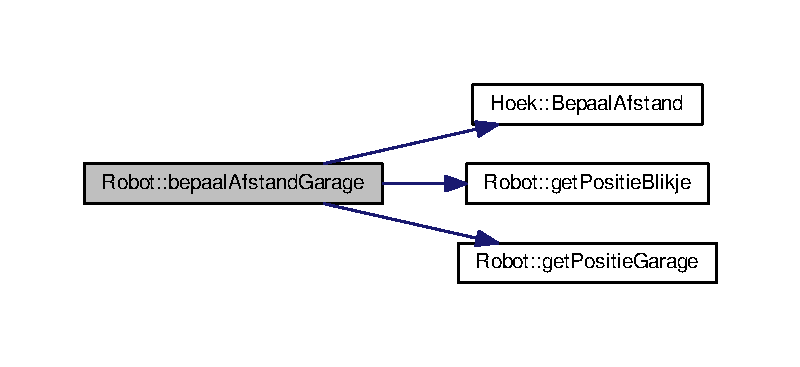
\includegraphics[width=350pt]{classRobot_a212f7383710351d161f084720aac00ad_cgraph}
\end{center}
\end{figure}


\hypertarget{classRobot_a1cbfcc8e3580c8ac369dc696dbdd640c}{\index{Robot@{Robot}!bepaal\-Hoek\-Blikje@{bepaal\-Hoek\-Blikje}}
\index{bepaal\-Hoek\-Blikje@{bepaal\-Hoek\-Blikje}!Robot@{Robot}}
\subsubsection[{bepaal\-Hoek\-Blikje}]{\setlength{\rightskip}{0pt plus 5cm}void Robot\-::bepaal\-Hoek\-Blikje (
\begin{DoxyParamCaption}
{}
\end{DoxyParamCaption}
)}}\label{classRobot_a1cbfcc8e3580c8ac369dc696dbdd640c}


Here is the call graph for this function\-:
\nopagebreak
\begin{figure}[H]
\begin{center}
\leavevmode
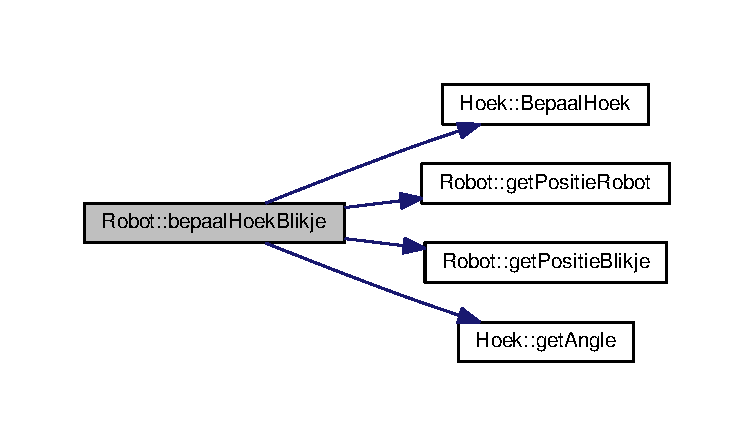
\includegraphics[width=350pt]{classRobot_a1cbfcc8e3580c8ac369dc696dbdd640c_cgraph}
\end{center}
\end{figure}


\hypertarget{classRobot_a5b40bae7bd0b458676caf2f5288d2047}{\index{Robot@{Robot}!bepaal\-Hoek\-Garage@{bepaal\-Hoek\-Garage}}
\index{bepaal\-Hoek\-Garage@{bepaal\-Hoek\-Garage}!Robot@{Robot}}
\subsubsection[{bepaal\-Hoek\-Garage}]{\setlength{\rightskip}{0pt plus 5cm}void Robot\-::bepaal\-Hoek\-Garage (
\begin{DoxyParamCaption}
{}
\end{DoxyParamCaption}
)}}\label{classRobot_a5b40bae7bd0b458676caf2f5288d2047}


Here is the call graph for this function\-:
\nopagebreak
\begin{figure}[H]
\begin{center}
\leavevmode
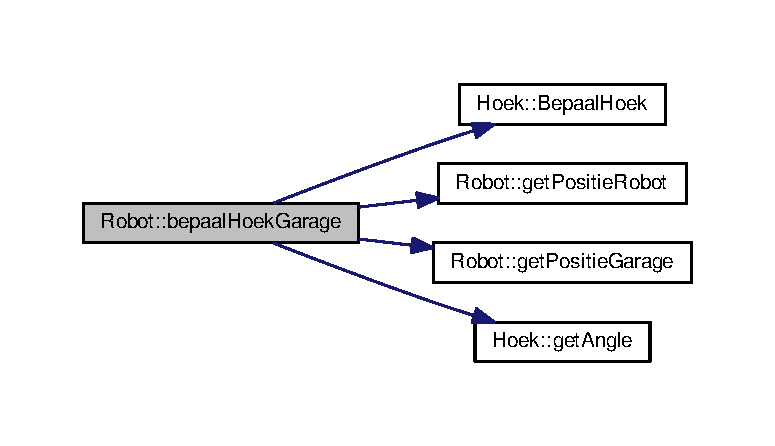
\includegraphics[width=350pt]{classRobot_a5b40bae7bd0b458676caf2f5288d2047_cgraph}
\end{center}
\end{figure}


\hypertarget{classRobot_ab6fc311f9a66f524aac0757a7b2a4a57}{\index{Robot@{Robot}!blikje\-Verplaatst@{blikje\-Verplaatst}}
\index{blikje\-Verplaatst@{blikje\-Verplaatst}!Robot@{Robot}}
\subsubsection[{blikje\-Verplaatst}]{\setlength{\rightskip}{0pt plus 5cm}bool Robot\-::blikje\-Verplaatst (
\begin{DoxyParamCaption}
{}
\end{DoxyParamCaption}
)}}\label{classRobot_ab6fc311f9a66f524aac0757a7b2a4a57}
\hypertarget{classRobot_abfab62ce2a3ff22f237e34ad1a6650e7}{\index{Robot@{Robot}!get\-Positie\-Blikje@{get\-Positie\-Blikje}}
\index{get\-Positie\-Blikje@{get\-Positie\-Blikje}!Robot@{Robot}}
\subsubsection[{get\-Positie\-Blikje}]{\setlength{\rightskip}{0pt plus 5cm}{\bf Positie} Robot\-::get\-Positie\-Blikje (
\begin{DoxyParamCaption}
{}
\end{DoxyParamCaption}
)}}\label{classRobot_abfab62ce2a3ff22f237e34ad1a6650e7}
\hypertarget{classRobot_a9301d035810174edffb769fd097f2a0c}{\index{Robot@{Robot}!get\-Positie\-Garage@{get\-Positie\-Garage}}
\index{get\-Positie\-Garage@{get\-Positie\-Garage}!Robot@{Robot}}
\subsubsection[{get\-Positie\-Garage}]{\setlength{\rightskip}{0pt plus 5cm}{\bf Positie} Robot\-::get\-Positie\-Garage (
\begin{DoxyParamCaption}
{}
\end{DoxyParamCaption}
)}}\label{classRobot_a9301d035810174edffb769fd097f2a0c}
\hypertarget{classRobot_a43fdd19ef403be762d659593023dda8a}{\index{Robot@{Robot}!get\-Positie\-Robot@{get\-Positie\-Robot}}
\index{get\-Positie\-Robot@{get\-Positie\-Robot}!Robot@{Robot}}
\subsubsection[{get\-Positie\-Robot}]{\setlength{\rightskip}{0pt plus 5cm}{\bf Positie} Robot\-::get\-Positie\-Robot (
\begin{DoxyParamCaption}
{}
\end{DoxyParamCaption}
)}}\label{classRobot_a43fdd19ef403be762d659593023dda8a}
\hypertarget{classRobot_a4895306b538817f9044c1b9b69e89781}{\index{Robot@{Robot}!print@{print}}
\index{print@{print}!Robot@{Robot}}
\subsubsection[{print}]{\setlength{\rightskip}{0pt plus 5cm}void Robot\-::print (
\begin{DoxyParamCaption}
{}
\end{DoxyParamCaption}
)}}\label{classRobot_a4895306b538817f9044c1b9b69e89781}


Here is the call graph for this function\-:
\nopagebreak
\begin{figure}[H]
\begin{center}
\leavevmode
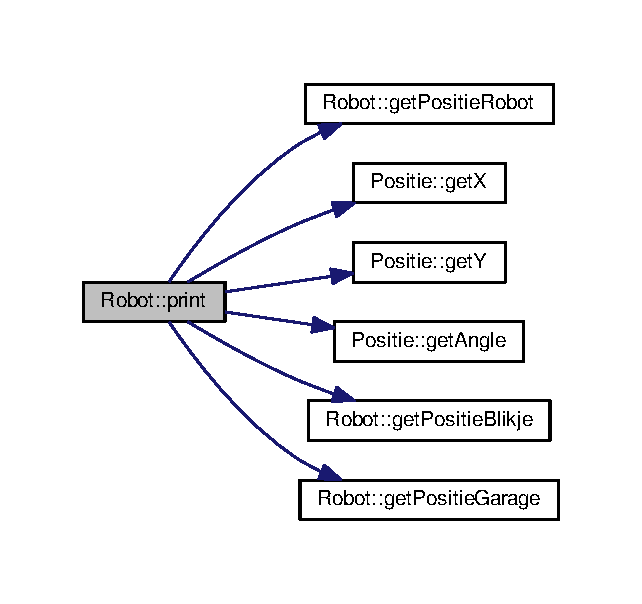
\includegraphics[width=308pt]{classRobot_a4895306b538817f9044c1b9b69e89781_cgraph}
\end{center}
\end{figure}


\hypertarget{classRobot_a17c05db895bbe8696acb2e0079f68de0}{\index{Robot@{Robot}!set\-Initiele\-Pos\-Blikje\-Geset@{set\-Initiele\-Pos\-Blikje\-Geset}}
\index{set\-Initiele\-Pos\-Blikje\-Geset@{set\-Initiele\-Pos\-Blikje\-Geset}!Robot@{Robot}}
\subsubsection[{set\-Initiele\-Pos\-Blikje\-Geset}]{\setlength{\rightskip}{0pt plus 5cm}void Robot\-::set\-Initiele\-Pos\-Blikje\-Geset (
\begin{DoxyParamCaption}
\item[{bool}]{b}
\end{DoxyParamCaption}
)}}\label{classRobot_a17c05db895bbe8696acb2e0079f68de0}
\hypertarget{classRobot_ad1c9b6e11cfb97e966350162ef38c7a2}{\index{Robot@{Robot}!set\-Positie\-Blikje@{set\-Positie\-Blikje}}
\index{set\-Positie\-Blikje@{set\-Positie\-Blikje}!Robot@{Robot}}
\subsubsection[{set\-Positie\-Blikje}]{\setlength{\rightskip}{0pt plus 5cm}void Robot\-::set\-Positie\-Blikje (
\begin{DoxyParamCaption}
\item[{{\bf Positie}}]{val}
\end{DoxyParamCaption}
)}}\label{classRobot_ad1c9b6e11cfb97e966350162ef38c7a2}
\hypertarget{classRobot_a29185fbf1e17fe20b357afb1753bb29e}{\index{Robot@{Robot}!set\-Positie\-Blikje@{set\-Positie\-Blikje}}
\index{set\-Positie\-Blikje@{set\-Positie\-Blikje}!Robot@{Robot}}
\subsubsection[{set\-Positie\-Blikje}]{\setlength{\rightskip}{0pt plus 5cm}void Robot\-::set\-Positie\-Blikje (
\begin{DoxyParamCaption}
\item[{int}]{x, }
\item[{int}]{y}
\end{DoxyParamCaption}
)}}\label{classRobot_a29185fbf1e17fe20b357afb1753bb29e}


Here is the call graph for this function\-:
\nopagebreak
\begin{figure}[H]
\begin{center}
\leavevmode
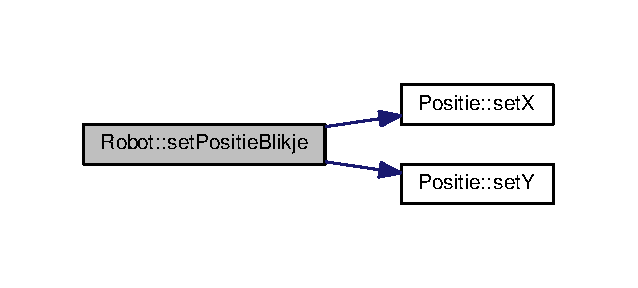
\includegraphics[width=306pt]{classRobot_a29185fbf1e17fe20b357afb1753bb29e_cgraph}
\end{center}
\end{figure}


\hypertarget{classRobot_affb796dc23ca48799c1fc9ab31f578d9}{\index{Robot@{Robot}!set\-Positie\-Garage@{set\-Positie\-Garage}}
\index{set\-Positie\-Garage@{set\-Positie\-Garage}!Robot@{Robot}}
\subsubsection[{set\-Positie\-Garage}]{\setlength{\rightskip}{0pt plus 5cm}void Robot\-::set\-Positie\-Garage (
\begin{DoxyParamCaption}
\item[{{\bf Positie}}]{val}
\end{DoxyParamCaption}
)}}\label{classRobot_affb796dc23ca48799c1fc9ab31f578d9}
\hypertarget{classRobot_a371cff32d467a1cbaf2a8d212921845a}{\index{Robot@{Robot}!set\-Positie\-Garage@{set\-Positie\-Garage}}
\index{set\-Positie\-Garage@{set\-Positie\-Garage}!Robot@{Robot}}
\subsubsection[{set\-Positie\-Garage}]{\setlength{\rightskip}{0pt plus 5cm}void Robot\-::set\-Positie\-Garage (
\begin{DoxyParamCaption}
\item[{int}]{x, }
\item[{int}]{y}
\end{DoxyParamCaption}
)}}\label{classRobot_a371cff32d467a1cbaf2a8d212921845a}


Here is the call graph for this function\-:
\nopagebreak
\begin{figure}[H]
\begin{center}
\leavevmode
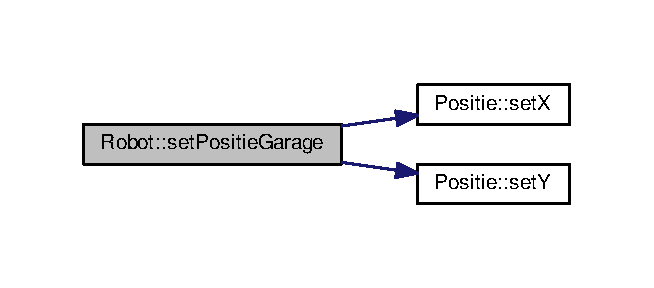
\includegraphics[width=314pt]{classRobot_a371cff32d467a1cbaf2a8d212921845a_cgraph}
\end{center}
\end{figure}


\hypertarget{classRobot_a6d3de1bc1f766693e4058a02a7744293}{\index{Robot@{Robot}!set\-Positie\-Robot@{set\-Positie\-Robot}}
\index{set\-Positie\-Robot@{set\-Positie\-Robot}!Robot@{Robot}}
\subsubsection[{set\-Positie\-Robot}]{\setlength{\rightskip}{0pt plus 5cm}void Robot\-::set\-Positie\-Robot (
\begin{DoxyParamCaption}
\item[{{\bf Positie}}]{val}
\end{DoxyParamCaption}
)}}\label{classRobot_a6d3de1bc1f766693e4058a02a7744293}
\hypertarget{classRobot_a3f35253e8b6e3810aa377c9f3c4158de}{\index{Robot@{Robot}!set\-Positie\-Robot@{set\-Positie\-Robot}}
\index{set\-Positie\-Robot@{set\-Positie\-Robot}!Robot@{Robot}}
\subsubsection[{set\-Positie\-Robot}]{\setlength{\rightskip}{0pt plus 5cm}void Robot\-::set\-Positie\-Robot (
\begin{DoxyParamCaption}
\item[{int}]{x, }
\item[{int}]{y, }
\item[{int}]{angle}
\end{DoxyParamCaption}
)}}\label{classRobot_a3f35253e8b6e3810aa377c9f3c4158de}


Here is the call graph for this function\-:
\nopagebreak
\begin{figure}[H]
\begin{center}
\leavevmode
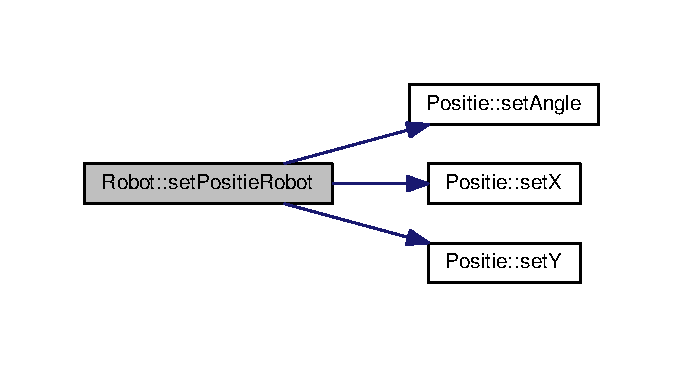
\includegraphics[width=328pt]{classRobot_a3f35253e8b6e3810aa377c9f3c4158de_cgraph}
\end{center}
\end{figure}


\hypertarget{classRobot_a980d1f972db40e5afcf3e2caf6ba346c}{\index{Robot@{Robot}!update\-Posities@{update\-Posities}}
\index{update\-Posities@{update\-Posities}!Robot@{Robot}}
\subsubsection[{update\-Posities}]{\setlength{\rightskip}{0pt plus 5cm}void Robot\-::update\-Posities (
\begin{DoxyParamCaption}
{}
\end{DoxyParamCaption}
)}}\label{classRobot_a980d1f972db40e5afcf3e2caf6ba346c}


Here is the call graph for this function\-:
\nopagebreak
\begin{figure}[H]
\begin{center}
\leavevmode
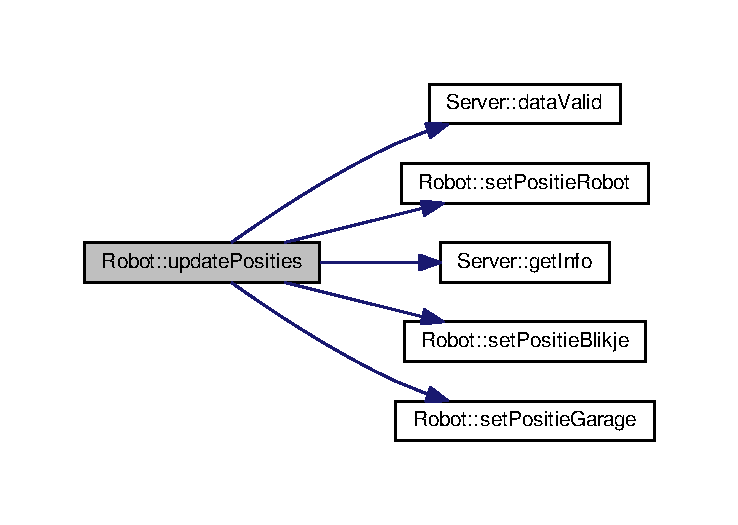
\includegraphics[width=350pt]{classRobot_a980d1f972db40e5afcf3e2caf6ba346c_cgraph}
\end{center}
\end{figure}




\subsection{Member Data Documentation}
\hypertarget{classRobot_a6914cbc8706b7a2096b39a3a059b31bf}{\index{Robot@{Robot}!avgposblikje@{avgposblikje}}
\index{avgposblikje@{avgposblikje}!Robot@{Robot}}
\subsubsection[{avgposblikje}]{\setlength{\rightskip}{0pt plus 5cm}{\bf Average} Robot\-::avgposblikje\hspace{0.3cm}{\ttfamily [private]}}}\label{classRobot_a6914cbc8706b7a2096b39a3a059b31bf}
\hypertarget{classRobot_ab74847d7cebe2e6141ec9ff00745594c}{\index{Robot@{Robot}!avgposgarage@{avgposgarage}}
\index{avgposgarage@{avgposgarage}!Robot@{Robot}}
\subsubsection[{avgposgarage}]{\setlength{\rightskip}{0pt plus 5cm}{\bf Average} Robot\-::avgposgarage\hspace{0.3cm}{\ttfamily [private]}}}\label{classRobot_ab74847d7cebe2e6141ec9ff00745594c}
\hypertarget{classRobot_afb0e831757aefcfe83bd3df04d8ab4e7}{\index{Robot@{Robot}!avgposrobot@{avgposrobot}}
\index{avgposrobot@{avgposrobot}!Robot@{Robot}}
\subsubsection[{avgposrobot}]{\setlength{\rightskip}{0pt plus 5cm}{\bf Average} Robot\-::avgposrobot\hspace{0.3cm}{\ttfamily [private]}}}\label{classRobot_afb0e831757aefcfe83bd3df04d8ab4e7}
\hypertarget{classRobot_a96f64e31d55c578095db9cd225597763}{\index{Robot@{Robot}!initiele\-Pos\-Blikje@{initiele\-Pos\-Blikje}}
\index{initiele\-Pos\-Blikje@{initiele\-Pos\-Blikje}!Robot@{Robot}}
\subsubsection[{initiele\-Pos\-Blikje}]{\setlength{\rightskip}{0pt plus 5cm}{\bf Positie} Robot\-::initiele\-Pos\-Blikje\hspace{0.3cm}{\ttfamily [private]}}}\label{classRobot_a96f64e31d55c578095db9cd225597763}
\hypertarget{classRobot_a89cba58927f6471cc51991ea6d1a5009}{\index{Robot@{Robot}!initiele\-Pos\-Blikje\-Geset@{initiele\-Pos\-Blikje\-Geset}}
\index{initiele\-Pos\-Blikje\-Geset@{initiele\-Pos\-Blikje\-Geset}!Robot@{Robot}}
\subsubsection[{initiele\-Pos\-Blikje\-Geset}]{\setlength{\rightskip}{0pt plus 5cm}bool Robot\-::initiele\-Pos\-Blikje\-Geset\hspace{0.3cm}{\ttfamily [private]}}}\label{classRobot_a89cba58927f6471cc51991ea6d1a5009}
\hypertarget{classRobot_a430b77999d3080962df243cc80ff41cc}{\index{Robot@{Robot}!pos\-Blikje@{pos\-Blikje}}
\index{pos\-Blikje@{pos\-Blikje}!Robot@{Robot}}
\subsubsection[{pos\-Blikje}]{\setlength{\rightskip}{0pt plus 5cm}{\bf Positie} Robot\-::pos\-Blikje\hspace{0.3cm}{\ttfamily [private]}}}\label{classRobot_a430b77999d3080962df243cc80ff41cc}
\hypertarget{classRobot_a65d03adc264ed54988a63793bd1ee9c5}{\index{Robot@{Robot}!pos\-Garage@{pos\-Garage}}
\index{pos\-Garage@{pos\-Garage}!Robot@{Robot}}
\subsubsection[{pos\-Garage}]{\setlength{\rightskip}{0pt plus 5cm}{\bf Positie} Robot\-::pos\-Garage\hspace{0.3cm}{\ttfamily [private]}}}\label{classRobot_a65d03adc264ed54988a63793bd1ee9c5}
\hypertarget{classRobot_a9d4895475ce429baafb7056bba91892d}{\index{Robot@{Robot}!pos\-Robot@{pos\-Robot}}
\index{pos\-Robot@{pos\-Robot}!Robot@{Robot}}
\subsubsection[{pos\-Robot}]{\setlength{\rightskip}{0pt plus 5cm}{\bf Positie} Robot\-::pos\-Robot\hspace{0.3cm}{\ttfamily [private]}}}\label{classRobot_a9d4895475ce429baafb7056bba91892d}


The documentation for this class was generated from the following files\-:\begin{DoxyCompactItemize}
\item 
include/\hyperlink{Robot_8h}{Robot.\-h}\item 
src/\hyperlink{Robot_8cpp}{Robot.\-cpp}\end{DoxyCompactItemize}

\hypertarget{classrobotcommand}{\section{robotcommand Class Reference}
\label{classrobotcommand}\index{robotcommand@{robotcommand}}
}


{\ttfamily \#include $<$robotcommand.\-h$>$}



Inheritance diagram for robotcommand\-:
\nopagebreak
\begin{figure}[H]
\begin{center}
\leavevmode
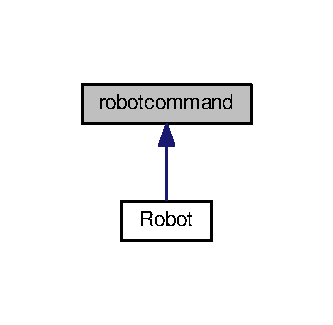
\includegraphics[width=160pt]{classrobotcommand__inherit__graph}
\end{center}
\end{figure}


Collaboration diagram for robotcommand\-:
\nopagebreak
\begin{figure}[H]
\begin{center}
\leavevmode
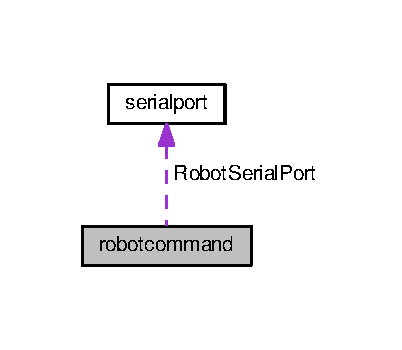
\includegraphics[width=193pt]{classrobotcommand__coll__graph}
\end{center}
\end{figure}
\subsection*{Public Member Functions}
\begin{DoxyCompactItemize}
\item 
\hyperlink{classrobotcommand_aa9baff763183ccfc69757aca4e40dcd8}{$\sim$robotcommand} ()
\item 
\hyperlink{classrobotcommand_af19fa9cf0701a23ab114b69e756d1ab5}{robotcommand} ()
\item 
\hyperlink{classrobotcommand_a52e24824353237ed366fc010a2fe83f1}{robotcommand} (string port=\hyperlink{robotcommand_8h_acd526f11ce51532b8187f63bac77d87b}{S\-E\-R\-I\-A\-L\-P\-O\-R\-T})
\item 
int \hyperlink{classrobotcommand_a108981093dc6edff9aa95b28b2cc2333}{turn\-Round\-Own\-Axis} (char direction, int angle)
\item 
int \hyperlink{classrobotcommand_a0ef498eb5ba8f4b25c5623c435af6239}{turn\-Direction} (char direction, int speed)
\item 
int \hyperlink{classrobotcommand_a9ac4f18967d91b8e509767dc9f21cde7}{drive\-Forward} (int speed)
\item 
int \hyperlink{classrobotcommand_a460b1282f139510ac5347415a996d961}{drive\-Reverse} (int speed)
\item 
int \hyperlink{classrobotcommand_a32699ec2e45ef5e6aaaab39a51e27a63}{stop} ()
\item 
int \hyperlink{classrobotcommand_a4213a394de57c5c24a976cc3e8c1717a}{get\-Drive\-State} ()
\item 
int \hyperlink{classrobotcommand_af741cb165c3871d9d0503f56fa3c78b1}{grip\-Open} ()
\item 
int \hyperlink{classrobotcommand_a076218b7721984dacd431594dd03f420}{grip\-Close} ()
\item 
int \hyperlink{classrobotcommand_a69294589313aa0a1d7a03d9f3dc7656f}{get\-Grip\-State} ()
\item 
int \hyperlink{classrobotcommand_ad10998d94d1b7f378f0715b08b4efa2a}{read\-Distance} ()
\item 
int \hyperlink{classrobotcommand_a23fdf87741ce41a862dd0c9be64621a4}{read\-Voltage} ()
\item 
int \hyperlink{classrobotcommand_abe3d7070fde985f906c2f604d98ca1b2}{test\-Start\-Turn} ()
\end{DoxyCompactItemize}
\subsection*{Private Member Functions}
\begin{DoxyCompactItemize}
\item 
string \hyperlink{classrobotcommand_acedd5f9a9dc4a4a0965f46750eb8df33}{int\-To\-String} (int number)
\item 
int \hyperlink{classrobotcommand_a3bc304d1666269cc31f8ba929ba05d6d}{string\-To\-Int} (string txt)
\item 
int \hyperlink{classrobotcommand_ac254ab4292788bbf36667463dafd4c4c}{turn\-Round\-Own\-Axis} (char direction, int angle, int speed)
\end{DoxyCompactItemize}
\subsection*{Private Attributes}
\begin{DoxyCompactItemize}
\item 
\hyperlink{classserialport}{serialport} $\ast$ \hyperlink{classrobotcommand_ab4775e1be7dcbea9fcb686001e0d58a1}{Robot\-Serial\-Port}
\item 
bool \hyperlink{classrobotcommand_af5bfa13fcb7d45b8812e5c1f4a4cdfbb}{gripstate}
\item 
int \hyperlink{classrobotcommand_a4d67204c88b917ad8e395abb5f1384c7}{drivestate}
\end{DoxyCompactItemize}


\subsection{Constructor \& Destructor Documentation}
\hypertarget{classrobotcommand_aa9baff763183ccfc69757aca4e40dcd8}{\index{robotcommand@{robotcommand}!$\sim$robotcommand@{$\sim$robotcommand}}
\index{$\sim$robotcommand@{$\sim$robotcommand}!robotcommand@{robotcommand}}
\subsubsection[{$\sim$robotcommand}]{\setlength{\rightskip}{0pt plus 5cm}robotcommand\-::$\sim$robotcommand (
\begin{DoxyParamCaption}
{}
\end{DoxyParamCaption}
)}}\label{classrobotcommand_aa9baff763183ccfc69757aca4e40dcd8}
\hypertarget{classrobotcommand_af19fa9cf0701a23ab114b69e756d1ab5}{\index{robotcommand@{robotcommand}!robotcommand@{robotcommand}}
\index{robotcommand@{robotcommand}!robotcommand@{robotcommand}}
\subsubsection[{robotcommand}]{\setlength{\rightskip}{0pt plus 5cm}robotcommand\-::robotcommand (
\begin{DoxyParamCaption}
{}
\end{DoxyParamCaption}
)}}\label{classrobotcommand_af19fa9cf0701a23ab114b69e756d1ab5}
\hypertarget{classrobotcommand_a52e24824353237ed366fc010a2fe83f1}{\index{robotcommand@{robotcommand}!robotcommand@{robotcommand}}
\index{robotcommand@{robotcommand}!robotcommand@{robotcommand}}
\subsubsection[{robotcommand}]{\setlength{\rightskip}{0pt plus 5cm}robotcommand\-::robotcommand (
\begin{DoxyParamCaption}
\item[{string}]{port = {\ttfamily {\bf S\-E\-R\-I\-A\-L\-P\-O\-R\-T}}}
\end{DoxyParamCaption}
)}}\label{classrobotcommand_a52e24824353237ed366fc010a2fe83f1}


\subsection{Member Function Documentation}
\hypertarget{classrobotcommand_a9ac4f18967d91b8e509767dc9f21cde7}{\index{robotcommand@{robotcommand}!drive\-Forward@{drive\-Forward}}
\index{drive\-Forward@{drive\-Forward}!robotcommand@{robotcommand}}
\subsubsection[{drive\-Forward}]{\setlength{\rightskip}{0pt plus 5cm}int robotcommand\-::drive\-Forward (
\begin{DoxyParamCaption}
\item[{int}]{speed}
\end{DoxyParamCaption}
)}}\label{classrobotcommand_a9ac4f18967d91b8e509767dc9f21cde7}
\hypertarget{classrobotcommand_a460b1282f139510ac5347415a996d961}{\index{robotcommand@{robotcommand}!drive\-Reverse@{drive\-Reverse}}
\index{drive\-Reverse@{drive\-Reverse}!robotcommand@{robotcommand}}
\subsubsection[{drive\-Reverse}]{\setlength{\rightskip}{0pt plus 5cm}int robotcommand\-::drive\-Reverse (
\begin{DoxyParamCaption}
\item[{int}]{speed}
\end{DoxyParamCaption}
)}}\label{classrobotcommand_a460b1282f139510ac5347415a996d961}
\hypertarget{classrobotcommand_a4213a394de57c5c24a976cc3e8c1717a}{\index{robotcommand@{robotcommand}!get\-Drive\-State@{get\-Drive\-State}}
\index{get\-Drive\-State@{get\-Drive\-State}!robotcommand@{robotcommand}}
\subsubsection[{get\-Drive\-State}]{\setlength{\rightskip}{0pt plus 5cm}int robotcommand\-::get\-Drive\-State (
\begin{DoxyParamCaption}
{}
\end{DoxyParamCaption}
)}}\label{classrobotcommand_a4213a394de57c5c24a976cc3e8c1717a}
\hypertarget{classrobotcommand_a69294589313aa0a1d7a03d9f3dc7656f}{\index{robotcommand@{robotcommand}!get\-Grip\-State@{get\-Grip\-State}}
\index{get\-Grip\-State@{get\-Grip\-State}!robotcommand@{robotcommand}}
\subsubsection[{get\-Grip\-State}]{\setlength{\rightskip}{0pt plus 5cm}int robotcommand\-::get\-Grip\-State (
\begin{DoxyParamCaption}
{}
\end{DoxyParamCaption}
)}}\label{classrobotcommand_a69294589313aa0a1d7a03d9f3dc7656f}
\hypertarget{classrobotcommand_a076218b7721984dacd431594dd03f420}{\index{robotcommand@{robotcommand}!grip\-Close@{grip\-Close}}
\index{grip\-Close@{grip\-Close}!robotcommand@{robotcommand}}
\subsubsection[{grip\-Close}]{\setlength{\rightskip}{0pt plus 5cm}int robotcommand\-::grip\-Close (
\begin{DoxyParamCaption}
{}
\end{DoxyParamCaption}
)}}\label{classrobotcommand_a076218b7721984dacd431594dd03f420}
\hypertarget{classrobotcommand_af741cb165c3871d9d0503f56fa3c78b1}{\index{robotcommand@{robotcommand}!grip\-Open@{grip\-Open}}
\index{grip\-Open@{grip\-Open}!robotcommand@{robotcommand}}
\subsubsection[{grip\-Open}]{\setlength{\rightskip}{0pt plus 5cm}int robotcommand\-::grip\-Open (
\begin{DoxyParamCaption}
{}
\end{DoxyParamCaption}
)}}\label{classrobotcommand_af741cb165c3871d9d0503f56fa3c78b1}
\hypertarget{classrobotcommand_acedd5f9a9dc4a4a0965f46750eb8df33}{\index{robotcommand@{robotcommand}!int\-To\-String@{int\-To\-String}}
\index{int\-To\-String@{int\-To\-String}!robotcommand@{robotcommand}}
\subsubsection[{int\-To\-String}]{\setlength{\rightskip}{0pt plus 5cm}string robotcommand\-::int\-To\-String (
\begin{DoxyParamCaption}
\item[{int}]{number}
\end{DoxyParamCaption}
)\hspace{0.3cm}{\ttfamily [private]}}}\label{classrobotcommand_acedd5f9a9dc4a4a0965f46750eb8df33}
\hypertarget{classrobotcommand_ad10998d94d1b7f378f0715b08b4efa2a}{\index{robotcommand@{robotcommand}!read\-Distance@{read\-Distance}}
\index{read\-Distance@{read\-Distance}!robotcommand@{robotcommand}}
\subsubsection[{read\-Distance}]{\setlength{\rightskip}{0pt plus 5cm}int robotcommand\-::read\-Distance (
\begin{DoxyParamCaption}
{}
\end{DoxyParamCaption}
)}}\label{classrobotcommand_ad10998d94d1b7f378f0715b08b4efa2a}
\hypertarget{classrobotcommand_a23fdf87741ce41a862dd0c9be64621a4}{\index{robotcommand@{robotcommand}!read\-Voltage@{read\-Voltage}}
\index{read\-Voltage@{read\-Voltage}!robotcommand@{robotcommand}}
\subsubsection[{read\-Voltage}]{\setlength{\rightskip}{0pt plus 5cm}int robotcommand\-::read\-Voltage (
\begin{DoxyParamCaption}
{}
\end{DoxyParamCaption}
)}}\label{classrobotcommand_a23fdf87741ce41a862dd0c9be64621a4}
\hypertarget{classrobotcommand_a32699ec2e45ef5e6aaaab39a51e27a63}{\index{robotcommand@{robotcommand}!stop@{stop}}
\index{stop@{stop}!robotcommand@{robotcommand}}
\subsubsection[{stop}]{\setlength{\rightskip}{0pt plus 5cm}int robotcommand\-::stop (
\begin{DoxyParamCaption}
{}
\end{DoxyParamCaption}
)}}\label{classrobotcommand_a32699ec2e45ef5e6aaaab39a51e27a63}
\hypertarget{classrobotcommand_a3bc304d1666269cc31f8ba929ba05d6d}{\index{robotcommand@{robotcommand}!string\-To\-Int@{string\-To\-Int}}
\index{string\-To\-Int@{string\-To\-Int}!robotcommand@{robotcommand}}
\subsubsection[{string\-To\-Int}]{\setlength{\rightskip}{0pt plus 5cm}int robotcommand\-::string\-To\-Int (
\begin{DoxyParamCaption}
\item[{string}]{txt}
\end{DoxyParamCaption}
)\hspace{0.3cm}{\ttfamily [private]}}}\label{classrobotcommand_a3bc304d1666269cc31f8ba929ba05d6d}
\hypertarget{classrobotcommand_abe3d7070fde985f906c2f604d98ca1b2}{\index{robotcommand@{robotcommand}!test\-Start\-Turn@{test\-Start\-Turn}}
\index{test\-Start\-Turn@{test\-Start\-Turn}!robotcommand@{robotcommand}}
\subsubsection[{test\-Start\-Turn}]{\setlength{\rightskip}{0pt plus 5cm}int robotcommand\-::test\-Start\-Turn (
\begin{DoxyParamCaption}
{}
\end{DoxyParamCaption}
)}}\label{classrobotcommand_abe3d7070fde985f906c2f604d98ca1b2}
\hypertarget{classrobotcommand_a0ef498eb5ba8f4b25c5623c435af6239}{\index{robotcommand@{robotcommand}!turn\-Direction@{turn\-Direction}}
\index{turn\-Direction@{turn\-Direction}!robotcommand@{robotcommand}}
\subsubsection[{turn\-Direction}]{\setlength{\rightskip}{0pt plus 5cm}int robotcommand\-::turn\-Direction (
\begin{DoxyParamCaption}
\item[{char}]{direction, }
\item[{int}]{speed}
\end{DoxyParamCaption}
)}}\label{classrobotcommand_a0ef498eb5ba8f4b25c5623c435af6239}
\hypertarget{classrobotcommand_ac254ab4292788bbf36667463dafd4c4c}{\index{robotcommand@{robotcommand}!turn\-Round\-Own\-Axis@{turn\-Round\-Own\-Axis}}
\index{turn\-Round\-Own\-Axis@{turn\-Round\-Own\-Axis}!robotcommand@{robotcommand}}
\subsubsection[{turn\-Round\-Own\-Axis}]{\setlength{\rightskip}{0pt plus 5cm}int robotcommand\-::turn\-Round\-Own\-Axis (
\begin{DoxyParamCaption}
\item[{char}]{direction, }
\item[{int}]{angle, }
\item[{int}]{speed}
\end{DoxyParamCaption}
)\hspace{0.3cm}{\ttfamily [private]}}}\label{classrobotcommand_ac254ab4292788bbf36667463dafd4c4c}
\hypertarget{classrobotcommand_a108981093dc6edff9aa95b28b2cc2333}{\index{robotcommand@{robotcommand}!turn\-Round\-Own\-Axis@{turn\-Round\-Own\-Axis}}
\index{turn\-Round\-Own\-Axis@{turn\-Round\-Own\-Axis}!robotcommand@{robotcommand}}
\subsubsection[{turn\-Round\-Own\-Axis}]{\setlength{\rightskip}{0pt plus 5cm}int robotcommand\-::turn\-Round\-Own\-Axis (
\begin{DoxyParamCaption}
\item[{char}]{direction, }
\item[{int}]{angle}
\end{DoxyParamCaption}
)}}\label{classrobotcommand_a108981093dc6edff9aa95b28b2cc2333}


\subsection{Member Data Documentation}
\hypertarget{classrobotcommand_a4d67204c88b917ad8e395abb5f1384c7}{\index{robotcommand@{robotcommand}!drivestate@{drivestate}}
\index{drivestate@{drivestate}!robotcommand@{robotcommand}}
\subsubsection[{drivestate}]{\setlength{\rightskip}{0pt plus 5cm}int robotcommand\-::drivestate\hspace{0.3cm}{\ttfamily [private]}}}\label{classrobotcommand_a4d67204c88b917ad8e395abb5f1384c7}
\hypertarget{classrobotcommand_af5bfa13fcb7d45b8812e5c1f4a4cdfbb}{\index{robotcommand@{robotcommand}!gripstate@{gripstate}}
\index{gripstate@{gripstate}!robotcommand@{robotcommand}}
\subsubsection[{gripstate}]{\setlength{\rightskip}{0pt plus 5cm}bool robotcommand\-::gripstate\hspace{0.3cm}{\ttfamily [private]}}}\label{classrobotcommand_af5bfa13fcb7d45b8812e5c1f4a4cdfbb}
\hypertarget{classrobotcommand_ab4775e1be7dcbea9fcb686001e0d58a1}{\index{robotcommand@{robotcommand}!Robot\-Serial\-Port@{Robot\-Serial\-Port}}
\index{Robot\-Serial\-Port@{Robot\-Serial\-Port}!robotcommand@{robotcommand}}
\subsubsection[{Robot\-Serial\-Port}]{\setlength{\rightskip}{0pt plus 5cm}{\bf serialport}$\ast$ robotcommand\-::\-Robot\-Serial\-Port\hspace{0.3cm}{\ttfamily [private]}}}\label{classrobotcommand_ab4775e1be7dcbea9fcb686001e0d58a1}


The documentation for this class was generated from the following files\-:\begin{DoxyCompactItemize}
\item 
include/\hyperlink{robotcommand_8h}{robotcommand.\-h}\item 
src/\hyperlink{robotcommand_8cpp}{robotcommand.\-cpp}\end{DoxyCompactItemize}

\hypertarget{classserialport}{\section{serialport Class Reference}
\label{classserialport}\index{serialport@{serialport}}
}


{\ttfamily \#include $<$serialport.\-h$>$}

\subsection*{Public Member Functions}
\begin{DoxyCompactItemize}
\item 
\hyperlink{classserialport_ab6548ae7a7dcdb343e838140c8dfac9e}{$\sim$serialport} ()
\item 
\hyperlink{classserialport_a13b9a65e668dfd43f059c4e7b0e338fa}{serialport} (string port=\hyperlink{serialport_8h_a614217d263be1fb1a5f76e2ff7be19a2}{P\-O\-R\-T})
\item 
void \hyperlink{classserialport_ae2b84921379b9b43f2f8533c1374f443}{clear\-Buffer} ()
\item 
int \hyperlink{classserialport_ad2ef385508f2b121b90113c0b52b9b12}{s\-Write} (string)
\item 
int \hyperlink{classserialport_a5b840874cc3c361824051428f05a2d1c}{s\-Read} (char $\ast$)
\end{DoxyCompactItemize}
\subsection*{Private Attributes}
\begin{DoxyCompactItemize}
\item 
int \hyperlink{classserialport_ac0f432659cd8e2a2a05a7d8583d73968}{fd}
\item 
int \hyperlink{classserialport_ac2fa330c6a6d254fcda6e327eac6a7e7}{portopen}
\end{DoxyCompactItemize}


\subsection{Constructor \& Destructor Documentation}
\hypertarget{classserialport_ab6548ae7a7dcdb343e838140c8dfac9e}{\index{serialport@{serialport}!$\sim$serialport@{$\sim$serialport}}
\index{$\sim$serialport@{$\sim$serialport}!serialport@{serialport}}
\subsubsection[{$\sim$serialport}]{\setlength{\rightskip}{0pt plus 5cm}serialport\-::$\sim$serialport (
\begin{DoxyParamCaption}
{}
\end{DoxyParamCaption}
)}}\label{classserialport_ab6548ae7a7dcdb343e838140c8dfac9e}
\hypertarget{classserialport_a13b9a65e668dfd43f059c4e7b0e338fa}{\index{serialport@{serialport}!serialport@{serialport}}
\index{serialport@{serialport}!serialport@{serialport}}
\subsubsection[{serialport}]{\setlength{\rightskip}{0pt plus 5cm}serialport\-::serialport (
\begin{DoxyParamCaption}
\item[{string}]{port = {\ttfamily {\bf P\-O\-R\-T}}}
\end{DoxyParamCaption}
)}}\label{classserialport_a13b9a65e668dfd43f059c4e7b0e338fa}


\subsection{Member Function Documentation}
\hypertarget{classserialport_ae2b84921379b9b43f2f8533c1374f443}{\index{serialport@{serialport}!clear\-Buffer@{clear\-Buffer}}
\index{clear\-Buffer@{clear\-Buffer}!serialport@{serialport}}
\subsubsection[{clear\-Buffer}]{\setlength{\rightskip}{0pt plus 5cm}void serialport\-::clear\-Buffer (
\begin{DoxyParamCaption}
{}
\end{DoxyParamCaption}
)}}\label{classserialport_ae2b84921379b9b43f2f8533c1374f443}
\hypertarget{classserialport_a5b840874cc3c361824051428f05a2d1c}{\index{serialport@{serialport}!s\-Read@{s\-Read}}
\index{s\-Read@{s\-Read}!serialport@{serialport}}
\subsubsection[{s\-Read}]{\setlength{\rightskip}{0pt plus 5cm}int serialport\-::s\-Read (
\begin{DoxyParamCaption}
\item[{char $\ast$}]{bufferstring}
\end{DoxyParamCaption}
)}}\label{classserialport_a5b840874cc3c361824051428f05a2d1c}
\hypertarget{classserialport_ad2ef385508f2b121b90113c0b52b9b12}{\index{serialport@{serialport}!s\-Write@{s\-Write}}
\index{s\-Write@{s\-Write}!serialport@{serialport}}
\subsubsection[{s\-Write}]{\setlength{\rightskip}{0pt plus 5cm}int serialport\-::s\-Write (
\begin{DoxyParamCaption}
\item[{string}]{command}
\end{DoxyParamCaption}
)}}\label{classserialport_ad2ef385508f2b121b90113c0b52b9b12}


\subsection{Member Data Documentation}
\hypertarget{classserialport_ac0f432659cd8e2a2a05a7d8583d73968}{\index{serialport@{serialport}!fd@{fd}}
\index{fd@{fd}!serialport@{serialport}}
\subsubsection[{fd}]{\setlength{\rightskip}{0pt plus 5cm}int serialport\-::fd\hspace{0.3cm}{\ttfamily [private]}}}\label{classserialport_ac0f432659cd8e2a2a05a7d8583d73968}
\hypertarget{classserialport_ac2fa330c6a6d254fcda6e327eac6a7e7}{\index{serialport@{serialport}!portopen@{portopen}}
\index{portopen@{portopen}!serialport@{serialport}}
\subsubsection[{portopen}]{\setlength{\rightskip}{0pt plus 5cm}int serialport\-::portopen\hspace{0.3cm}{\ttfamily [private]}}}\label{classserialport_ac2fa330c6a6d254fcda6e327eac6a7e7}


The documentation for this class was generated from the following files\-:\begin{DoxyCompactItemize}
\item 
include/\hyperlink{serialport_8h}{serialport.\-h}\item 
src/\hyperlink{serialport_8cpp}{serialport.\-cpp}\end{DoxyCompactItemize}

\hypertarget{classServer}{\section{Server Class Reference}
\label{classServer}\index{Server@{Server}}
}


{\ttfamily \#include $<$Server.\-h$>$}



Inheritance diagram for Server\-:
\nopagebreak
\begin{figure}[H]
\begin{center}
\leavevmode
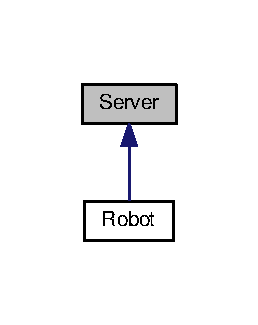
\includegraphics[width=124pt]{classServer__inherit__graph}
\end{center}
\end{figure}


Collaboration diagram for Server\-:
\nopagebreak
\begin{figure}[H]
\begin{center}
\leavevmode
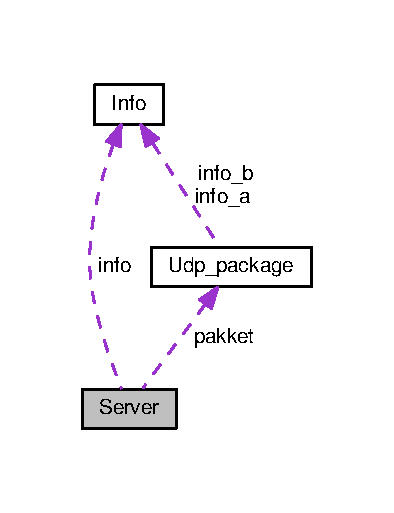
\includegraphics[width=189pt]{classServer__coll__graph}
\end{center}
\end{figure}
\subsection*{Public Member Functions}
\begin{DoxyCompactItemize}
\item 
\hyperlink{classServer_a4b3aa2579cb1c8cd1d069582c14d0fa6}{$\sim$\-Server} ()
\item 
\hyperlink{classServer_a81ef5528c64630e6c63bcfec1cc42317}{Server} (int port=\hyperlink{Server_8h_aba1a0da5373c381e0ad6481f8333c08a}{S\-T\-A\-N\-D\-A\-A\-R\-D\-P\-O\-O\-R\-T}, char c=\hyperlink{Server_8h_ab52a72e164e6995d7693a24dc3c43472}{S\-T\-A\-N\-D\-A\-A\-R\-D\-G\-R\-O\-E\-P})
\item 
void \hyperlink{classServer_ac2cf171fbcae23064b0139707e84a67c}{setup} ()
\item 
void \hyperlink{classServer_a83ae4701038e91258108a7701521cf78}{listen} ()
\item 
void \hyperlink{classServer_a972ee33b92b171ceb776e070ad892c98}{set\-Poort} (int port)
\item 
void \hyperlink{classServer_a7ce1f889e537ab405ad675b67d0f5380}{set\-Groep} (char c)
\item 
char \hyperlink{classServer_a25fc1f6dc4bf1bf674a416022587792a}{get\-Groep} ()
\item 
\hyperlink{structInfo}{Info} \hyperlink{classServer_a13eed202f15d451fa877233fcb58b5d4}{get\-Info} ()
\item 
bool \hyperlink{classServer_a162257cf71d621f37bd2fee3d554d029}{data\-Valid} ()
\end{DoxyCompactItemize}
\subsection*{Private Attributes}
\begin{DoxyCompactItemize}
\item 
int \hyperlink{classServer_a284abf5ae92eeed0f5e28759d382dd2d}{sockfd}
\item 
int \hyperlink{classServer_a60a838db7cee44ea45979e93c75137dd}{udp\-\_\-port}
\item 
\hyperlink{structInfo}{Info} \hyperlink{classServer_ae9d320c11dc676f6a24e41171bdd3beb}{info}
\item 
char \hyperlink{classServer_ae63c2574fcde32ea16b06b0bcb61b716}{groep}
\item 
struct sockaddr\-\_\-in \hyperlink{classServer_ac23e7b8d798bffefe61206636a8e1f57}{serveraddr}
\item 
struct sockaddr\-\_\-in \hyperlink{classServer_aa98c616c610a9f34a62b6c9f71ef7309}{clientaddr}
\item 
\hyperlink{structUdp__package}{Udp\-\_\-package} \hyperlink{classServer_a7850c5e7c92a04edbbd682d6553c18c8}{pakket}
\end{DoxyCompactItemize}


\subsection{Constructor \& Destructor Documentation}
\hypertarget{classServer_a4b3aa2579cb1c8cd1d069582c14d0fa6}{\index{Server@{Server}!$\sim$\-Server@{$\sim$\-Server}}
\index{$\sim$\-Server@{$\sim$\-Server}!Server@{Server}}
\subsubsection[{$\sim$\-Server}]{\setlength{\rightskip}{0pt plus 5cm}Server\-::$\sim$\-Server (
\begin{DoxyParamCaption}
{}
\end{DoxyParamCaption}
)}}\label{classServer_a4b3aa2579cb1c8cd1d069582c14d0fa6}
Destructor van \hyperlink{classServer}{Server} \hypertarget{classServer_a81ef5528c64630e6c63bcfec1cc42317}{\index{Server@{Server}!Server@{Server}}
\index{Server@{Server}!Server@{Server}}
\subsubsection[{Server}]{\setlength{\rightskip}{0pt plus 5cm}Server\-::\-Server (
\begin{DoxyParamCaption}
\item[{int}]{port = {\ttfamily {\bf S\-T\-A\-N\-D\-A\-A\-R\-D\-P\-O\-O\-R\-T}}, }
\item[{char}]{c = {\ttfamily {\bf S\-T\-A\-N\-D\-A\-A\-R\-D\-G\-R\-O\-E\-P}}}
\end{DoxyParamCaption}
)}}\label{classServer_a81ef5528c64630e6c63bcfec1cc42317}
Constructor van \hyperlink{classServer}{Server} 
\begin{DoxyParams}{Parameters}
{\em port} & U\-D\-P poort \\
\hline
{\em c} & groepsletter \\
\hline
\end{DoxyParams}


Here is the call graph for this function\-:
\nopagebreak
\begin{figure}[H]
\begin{center}
\leavevmode
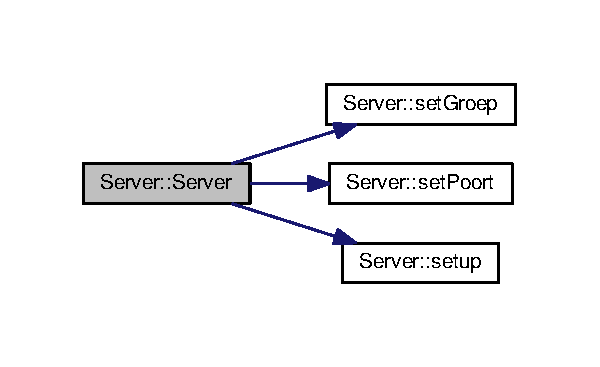
\includegraphics[width=288pt]{classServer_a81ef5528c64630e6c63bcfec1cc42317_cgraph}
\end{center}
\end{figure}




\subsection{Member Function Documentation}
\hypertarget{classServer_a162257cf71d621f37bd2fee3d554d029}{\index{Server@{Server}!data\-Valid@{data\-Valid}}
\index{data\-Valid@{data\-Valid}!Server@{Server}}
\subsubsection[{data\-Valid}]{\setlength{\rightskip}{0pt plus 5cm}bool Server\-::data\-Valid (
\begin{DoxyParamCaption}
{}
\end{DoxyParamCaption}
)}}\label{classServer_a162257cf71d621f37bd2fee3d554d029}
\begin{DoxyReturn}{Returns}

\end{DoxyReturn}
\hypertarget{classServer_a25fc1f6dc4bf1bf674a416022587792a}{\index{Server@{Server}!get\-Groep@{get\-Groep}}
\index{get\-Groep@{get\-Groep}!Server@{Server}}
\subsubsection[{get\-Groep}]{\setlength{\rightskip}{0pt plus 5cm}char Server\-::get\-Groep (
\begin{DoxyParamCaption}
{}
\end{DoxyParamCaption}
)}}\label{classServer_a25fc1f6dc4bf1bf674a416022587792a}
\begin{DoxyReturn}{Returns}

\end{DoxyReturn}
\hypertarget{classServer_a13eed202f15d451fa877233fcb58b5d4}{\index{Server@{Server}!get\-Info@{get\-Info}}
\index{get\-Info@{get\-Info}!Server@{Server}}
\subsubsection[{get\-Info}]{\setlength{\rightskip}{0pt plus 5cm}{\bf Info} Server\-::get\-Info (
\begin{DoxyParamCaption}
{}
\end{DoxyParamCaption}
)}}\label{classServer_a13eed202f15d451fa877233fcb58b5d4}
\begin{DoxyReturn}{Returns}

\end{DoxyReturn}
\hypertarget{classServer_a83ae4701038e91258108a7701521cf78}{\index{Server@{Server}!listen@{listen}}
\index{listen@{listen}!Server@{Server}}
\subsubsection[{listen}]{\setlength{\rightskip}{0pt plus 5cm}void Server\-::listen (
\begin{DoxyParamCaption}
{}
\end{DoxyParamCaption}
)}}\label{classServer_a83ae4701038e91258108a7701521cf78}


Here is the call graph for this function\-:
\nopagebreak
\begin{figure}[H]
\begin{center}
\leavevmode
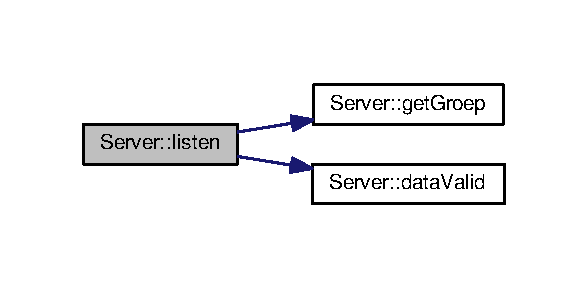
\includegraphics[width=282pt]{classServer_a83ae4701038e91258108a7701521cf78_cgraph}
\end{center}
\end{figure}


\hypertarget{classServer_a7ce1f889e537ab405ad675b67d0f5380}{\index{Server@{Server}!set\-Groep@{set\-Groep}}
\index{set\-Groep@{set\-Groep}!Server@{Server}}
\subsubsection[{set\-Groep}]{\setlength{\rightskip}{0pt plus 5cm}void Server\-::set\-Groep (
\begin{DoxyParamCaption}
\item[{char}]{c}
\end{DoxyParamCaption}
)}}\label{classServer_a7ce1f889e537ab405ad675b67d0f5380}

\begin{DoxyParams}{Parameters}
{\em c} & \\
\hline
\end{DoxyParams}
\hypertarget{classServer_a972ee33b92b171ceb776e070ad892c98}{\index{Server@{Server}!set\-Poort@{set\-Poort}}
\index{set\-Poort@{set\-Poort}!Server@{Server}}
\subsubsection[{set\-Poort}]{\setlength{\rightskip}{0pt plus 5cm}void Server\-::set\-Poort (
\begin{DoxyParamCaption}
\item[{int}]{port}
\end{DoxyParamCaption}
)}}\label{classServer_a972ee33b92b171ceb776e070ad892c98}

\begin{DoxyParams}{Parameters}
{\em port} & \\
\hline
\end{DoxyParams}
\hypertarget{classServer_ac2cf171fbcae23064b0139707e84a67c}{\index{Server@{Server}!setup@{setup}}
\index{setup@{setup}!Server@{Server}}
\subsubsection[{setup}]{\setlength{\rightskip}{0pt plus 5cm}void Server\-::setup (
\begin{DoxyParamCaption}
{}
\end{DoxyParamCaption}
)}}\label{classServer_ac2cf171fbcae23064b0139707e84a67c}


\subsection{Member Data Documentation}
\hypertarget{classServer_aa98c616c610a9f34a62b6c9f71ef7309}{\index{Server@{Server}!clientaddr@{clientaddr}}
\index{clientaddr@{clientaddr}!Server@{Server}}
\subsubsection[{clientaddr}]{\setlength{\rightskip}{0pt plus 5cm}struct sockaddr\-\_\-in Server\-::clientaddr\hspace{0.3cm}{\ttfamily [private]}}}\label{classServer_aa98c616c610a9f34a62b6c9f71ef7309}
\hypertarget{classServer_ae63c2574fcde32ea16b06b0bcb61b716}{\index{Server@{Server}!groep@{groep}}
\index{groep@{groep}!Server@{Server}}
\subsubsection[{groep}]{\setlength{\rightskip}{0pt plus 5cm}char Server\-::groep\hspace{0.3cm}{\ttfamily [private]}}}\label{classServer_ae63c2574fcde32ea16b06b0bcb61b716}
\hypertarget{classServer_ae9d320c11dc676f6a24e41171bdd3beb}{\index{Server@{Server}!info@{info}}
\index{info@{info}!Server@{Server}}
\subsubsection[{info}]{\setlength{\rightskip}{0pt plus 5cm}{\bf Info} Server\-::info\hspace{0.3cm}{\ttfamily [private]}}}\label{classServer_ae9d320c11dc676f6a24e41171bdd3beb}
\hypertarget{classServer_a7850c5e7c92a04edbbd682d6553c18c8}{\index{Server@{Server}!pakket@{pakket}}
\index{pakket@{pakket}!Server@{Server}}
\subsubsection[{pakket}]{\setlength{\rightskip}{0pt plus 5cm}{\bf Udp\-\_\-package} Server\-::pakket\hspace{0.3cm}{\ttfamily [private]}}}\label{classServer_a7850c5e7c92a04edbbd682d6553c18c8}
\hypertarget{classServer_ac23e7b8d798bffefe61206636a8e1f57}{\index{Server@{Server}!serveraddr@{serveraddr}}
\index{serveraddr@{serveraddr}!Server@{Server}}
\subsubsection[{serveraddr}]{\setlength{\rightskip}{0pt plus 5cm}struct sockaddr\-\_\-in Server\-::serveraddr\hspace{0.3cm}{\ttfamily [private]}}}\label{classServer_ac23e7b8d798bffefe61206636a8e1f57}
\hypertarget{classServer_a284abf5ae92eeed0f5e28759d382dd2d}{\index{Server@{Server}!sockfd@{sockfd}}
\index{sockfd@{sockfd}!Server@{Server}}
\subsubsection[{sockfd}]{\setlength{\rightskip}{0pt plus 5cm}int Server\-::sockfd\hspace{0.3cm}{\ttfamily [private]}}}\label{classServer_a284abf5ae92eeed0f5e28759d382dd2d}
\hypertarget{classServer_a60a838db7cee44ea45979e93c75137dd}{\index{Server@{Server}!udp\-\_\-port@{udp\-\_\-port}}
\index{udp\-\_\-port@{udp\-\_\-port}!Server@{Server}}
\subsubsection[{udp\-\_\-port}]{\setlength{\rightskip}{0pt plus 5cm}int Server\-::udp\-\_\-port\hspace{0.3cm}{\ttfamily [private]}}}\label{classServer_a60a838db7cee44ea45979e93c75137dd}


The documentation for this class was generated from the following files\-:\begin{DoxyCompactItemize}
\item 
include/\hyperlink{Server_8h}{Server.\-h}\item 
src/\hyperlink{Server_8cpp}{Server.\-cpp}\end{DoxyCompactItemize}

\hypertarget{structUdp__header}{\section{Udp\-\_\-header Struct Reference}
\label{structUdp__header}\index{Udp\-\_\-header@{Udp\-\_\-header}}
}


{\ttfamily \#include $<$Package.\-h$>$}

\subsection*{Public Attributes}
\begin{DoxyCompactItemize}
\item 
unsigned short int \hyperlink{structUdp__header_aa00a58023dd2a55db5b6e10d1a20a2a6}{udph\-\_\-srcport}
\item 
unsigned short int \hyperlink{structUdp__header_a4468a6ca345200bb93d91ceb4e1a7843}{udph\-\_\-destport}
\item 
unsigned short int \hyperlink{structUdp__header_aeff8dcbd93248830320fb64d5d056ae1}{udph\-\_\-len}
\item 
unsigned short int \hyperlink{structUdp__header_a7df7310126d017145fccb980dccd8752}{udph\-\_\-checksum}
\end{DoxyCompactItemize}


\subsection{Member Data Documentation}
\hypertarget{structUdp__header_a7df7310126d017145fccb980dccd8752}{\index{Udp\-\_\-header@{Udp\-\_\-header}!udph\-\_\-checksum@{udph\-\_\-checksum}}
\index{udph\-\_\-checksum@{udph\-\_\-checksum}!Udp_header@{Udp\-\_\-header}}
\subsubsection[{udph\-\_\-checksum}]{\setlength{\rightskip}{0pt plus 5cm}unsigned short int Udp\-\_\-header\-::udph\-\_\-checksum}}\label{structUdp__header_a7df7310126d017145fccb980dccd8752}
\hypertarget{structUdp__header_a4468a6ca345200bb93d91ceb4e1a7843}{\index{Udp\-\_\-header@{Udp\-\_\-header}!udph\-\_\-destport@{udph\-\_\-destport}}
\index{udph\-\_\-destport@{udph\-\_\-destport}!Udp_header@{Udp\-\_\-header}}
\subsubsection[{udph\-\_\-destport}]{\setlength{\rightskip}{0pt plus 5cm}unsigned short int Udp\-\_\-header\-::udph\-\_\-destport}}\label{structUdp__header_a4468a6ca345200bb93d91ceb4e1a7843}
\hypertarget{structUdp__header_aeff8dcbd93248830320fb64d5d056ae1}{\index{Udp\-\_\-header@{Udp\-\_\-header}!udph\-\_\-len@{udph\-\_\-len}}
\index{udph\-\_\-len@{udph\-\_\-len}!Udp_header@{Udp\-\_\-header}}
\subsubsection[{udph\-\_\-len}]{\setlength{\rightskip}{0pt plus 5cm}unsigned short int Udp\-\_\-header\-::udph\-\_\-len}}\label{structUdp__header_aeff8dcbd93248830320fb64d5d056ae1}
\hypertarget{structUdp__header_aa00a58023dd2a55db5b6e10d1a20a2a6}{\index{Udp\-\_\-header@{Udp\-\_\-header}!udph\-\_\-srcport@{udph\-\_\-srcport}}
\index{udph\-\_\-srcport@{udph\-\_\-srcport}!Udp_header@{Udp\-\_\-header}}
\subsubsection[{udph\-\_\-srcport}]{\setlength{\rightskip}{0pt plus 5cm}unsigned short int Udp\-\_\-header\-::udph\-\_\-srcport}}\label{structUdp__header_aa00a58023dd2a55db5b6e10d1a20a2a6}


The documentation for this struct was generated from the following file\-:\begin{DoxyCompactItemize}
\item 
include/\hyperlink{Package_8h}{Package.\-h}\end{DoxyCompactItemize}

\hypertarget{structUdp__package}{\section{Udp\-\_\-package Struct Reference}
\label{structUdp__package}\index{Udp\-\_\-package@{Udp\-\_\-package}}
}


{\ttfamily \#include $<$Package.\-h$>$}



Collaboration diagram for Udp\-\_\-package\-:
\nopagebreak
\begin{figure}[H]
\begin{center}
\leavevmode
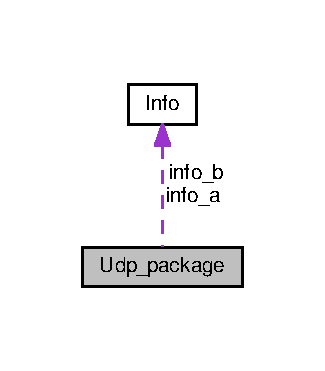
\includegraphics[width=156pt]{structUdp__package__coll__graph}
\end{center}
\end{figure}
\subsection*{Public Attributes}
\begin{DoxyCompactItemize}
\item 
int \hyperlink{structUdp__package_a970184a6e334fe29f4692718f271fdb0}{groep\-\_\-a}
\item 
\hyperlink{structInfo}{Info} \hyperlink{structUdp__package_a6cb537db96ffd959c77f135e44cfba3e}{info\-\_\-a}
\item 
int \hyperlink{structUdp__package_a8db8b9a082bf209e329b97a8a94cf690}{groep\-\_\-b}
\item 
\hyperlink{structInfo}{Info} \hyperlink{structUdp__package_ae1e5f1d35dfdae47b8750cbf4181bcac}{info\-\_\-b}
\item 
int \hyperlink{structUdp__package_a9b33ca73a59acb03b87d840a2086de68}{obs} \mbox{[}8\mbox{]}
\end{DoxyCompactItemize}


\subsection{Member Data Documentation}
\hypertarget{structUdp__package_a970184a6e334fe29f4692718f271fdb0}{\index{Udp\-\_\-package@{Udp\-\_\-package}!groep\-\_\-a@{groep\-\_\-a}}
\index{groep\-\_\-a@{groep\-\_\-a}!Udp_package@{Udp\-\_\-package}}
\subsubsection[{groep\-\_\-a}]{\setlength{\rightskip}{0pt plus 5cm}int Udp\-\_\-package\-::groep\-\_\-a}}\label{structUdp__package_a970184a6e334fe29f4692718f271fdb0}
\hypertarget{structUdp__package_a8db8b9a082bf209e329b97a8a94cf690}{\index{Udp\-\_\-package@{Udp\-\_\-package}!groep\-\_\-b@{groep\-\_\-b}}
\index{groep\-\_\-b@{groep\-\_\-b}!Udp_package@{Udp\-\_\-package}}
\subsubsection[{groep\-\_\-b}]{\setlength{\rightskip}{0pt plus 5cm}int Udp\-\_\-package\-::groep\-\_\-b}}\label{structUdp__package_a8db8b9a082bf209e329b97a8a94cf690}
\hypertarget{structUdp__package_a6cb537db96ffd959c77f135e44cfba3e}{\index{Udp\-\_\-package@{Udp\-\_\-package}!info\-\_\-a@{info\-\_\-a}}
\index{info\-\_\-a@{info\-\_\-a}!Udp_package@{Udp\-\_\-package}}
\subsubsection[{info\-\_\-a}]{\setlength{\rightskip}{0pt plus 5cm}{\bf Info} Udp\-\_\-package\-::info\-\_\-a}}\label{structUdp__package_a6cb537db96ffd959c77f135e44cfba3e}
\hypertarget{structUdp__package_ae1e5f1d35dfdae47b8750cbf4181bcac}{\index{Udp\-\_\-package@{Udp\-\_\-package}!info\-\_\-b@{info\-\_\-b}}
\index{info\-\_\-b@{info\-\_\-b}!Udp_package@{Udp\-\_\-package}}
\subsubsection[{info\-\_\-b}]{\setlength{\rightskip}{0pt plus 5cm}{\bf Info} Udp\-\_\-package\-::info\-\_\-b}}\label{structUdp__package_ae1e5f1d35dfdae47b8750cbf4181bcac}
\hypertarget{structUdp__package_a9b33ca73a59acb03b87d840a2086de68}{\index{Udp\-\_\-package@{Udp\-\_\-package}!obs@{obs}}
\index{obs@{obs}!Udp_package@{Udp\-\_\-package}}
\subsubsection[{obs}]{\setlength{\rightskip}{0pt plus 5cm}int Udp\-\_\-package\-::obs\mbox{[}8\mbox{]}}}\label{structUdp__package_a9b33ca73a59acb03b87d840a2086de68}


The documentation for this struct was generated from the following file\-:\begin{DoxyCompactItemize}
\item 
include/\hyperlink{Package_8h}{Package.\-h}\end{DoxyCompactItemize}

\chapter{File Documentation}
\hypertarget{Average_8h}{\section{include/\-Average.h File Reference}
\label{Average_8h}\index{include/\-Average.\-h@{include/\-Average.\-h}}
}
{\ttfamily \#include \char`\"{}debug.\-h\char`\"{}}\\*
{\ttfamily \#include \char`\"{}Positie.\-h\char`\"{}}\\*
Include dependency graph for Average.\-h\-:
\nopagebreak
\begin{figure}[H]
\begin{center}
\leavevmode
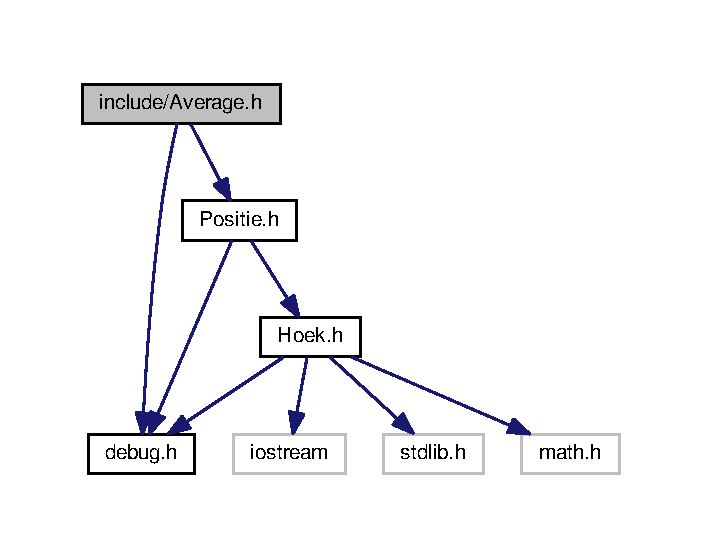
\includegraphics[width=337pt]{Average_8h__incl}
\end{center}
\end{figure}
This graph shows which files directly or indirectly include this file\-:
\nopagebreak
\begin{figure}[H]
\begin{center}
\leavevmode
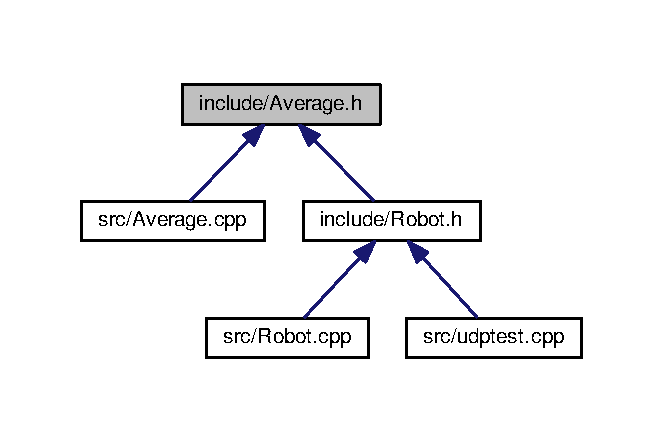
\includegraphics[width=319pt]{Average_8h__dep__incl}
\end{center}
\end{figure}
\subsection*{Classes}
\begin{DoxyCompactItemize}
\item 
class \hyperlink{classAverage}{Average}
\end{DoxyCompactItemize}
\subsection*{Macros}
\begin{DoxyCompactItemize}
\item 
\#define \hyperlink{Average_8h_a630b6d229997be7a86178cd718b70e54}{D\-E\-B\-U\-G\-A\-V\-E\-R\-A\-G\-E}
\item 
\#define \hyperlink{Average_8h_a70d1b7be16e53d5ab19ecfe0d11c888f}{N\-U\-M\-S\-A\-M\-P\-L\-E\-S}~8
\end{DoxyCompactItemize}


\subsection{Macro Definition Documentation}
\hypertarget{Average_8h_a630b6d229997be7a86178cd718b70e54}{\index{Average.\-h@{Average.\-h}!D\-E\-B\-U\-G\-A\-V\-E\-R\-A\-G\-E@{D\-E\-B\-U\-G\-A\-V\-E\-R\-A\-G\-E}}
\index{D\-E\-B\-U\-G\-A\-V\-E\-R\-A\-G\-E@{D\-E\-B\-U\-G\-A\-V\-E\-R\-A\-G\-E}!Average.h@{Average.\-h}}
\subsubsection[{D\-E\-B\-U\-G\-A\-V\-E\-R\-A\-G\-E}]{\setlength{\rightskip}{0pt plus 5cm}\#define D\-E\-B\-U\-G\-A\-V\-E\-R\-A\-G\-E}}\label{Average_8h_a630b6d229997be7a86178cd718b70e54}
\hypertarget{Average_8h_a70d1b7be16e53d5ab19ecfe0d11c888f}{\index{Average.\-h@{Average.\-h}!N\-U\-M\-S\-A\-M\-P\-L\-E\-S@{N\-U\-M\-S\-A\-M\-P\-L\-E\-S}}
\index{N\-U\-M\-S\-A\-M\-P\-L\-E\-S@{N\-U\-M\-S\-A\-M\-P\-L\-E\-S}!Average.h@{Average.\-h}}
\subsubsection[{N\-U\-M\-S\-A\-M\-P\-L\-E\-S}]{\setlength{\rightskip}{0pt plus 5cm}\#define N\-U\-M\-S\-A\-M\-P\-L\-E\-S~8}}\label{Average_8h_a70d1b7be16e53d5ab19ecfe0d11c888f}

\hypertarget{debug_8h}{\section{include/debug.h File Reference}
\label{debug_8h}\index{include/debug.\-h@{include/debug.\-h}}
}
This graph shows which files directly or indirectly include this file\-:
\nopagebreak
\begin{figure}[H]
\begin{center}
\leavevmode
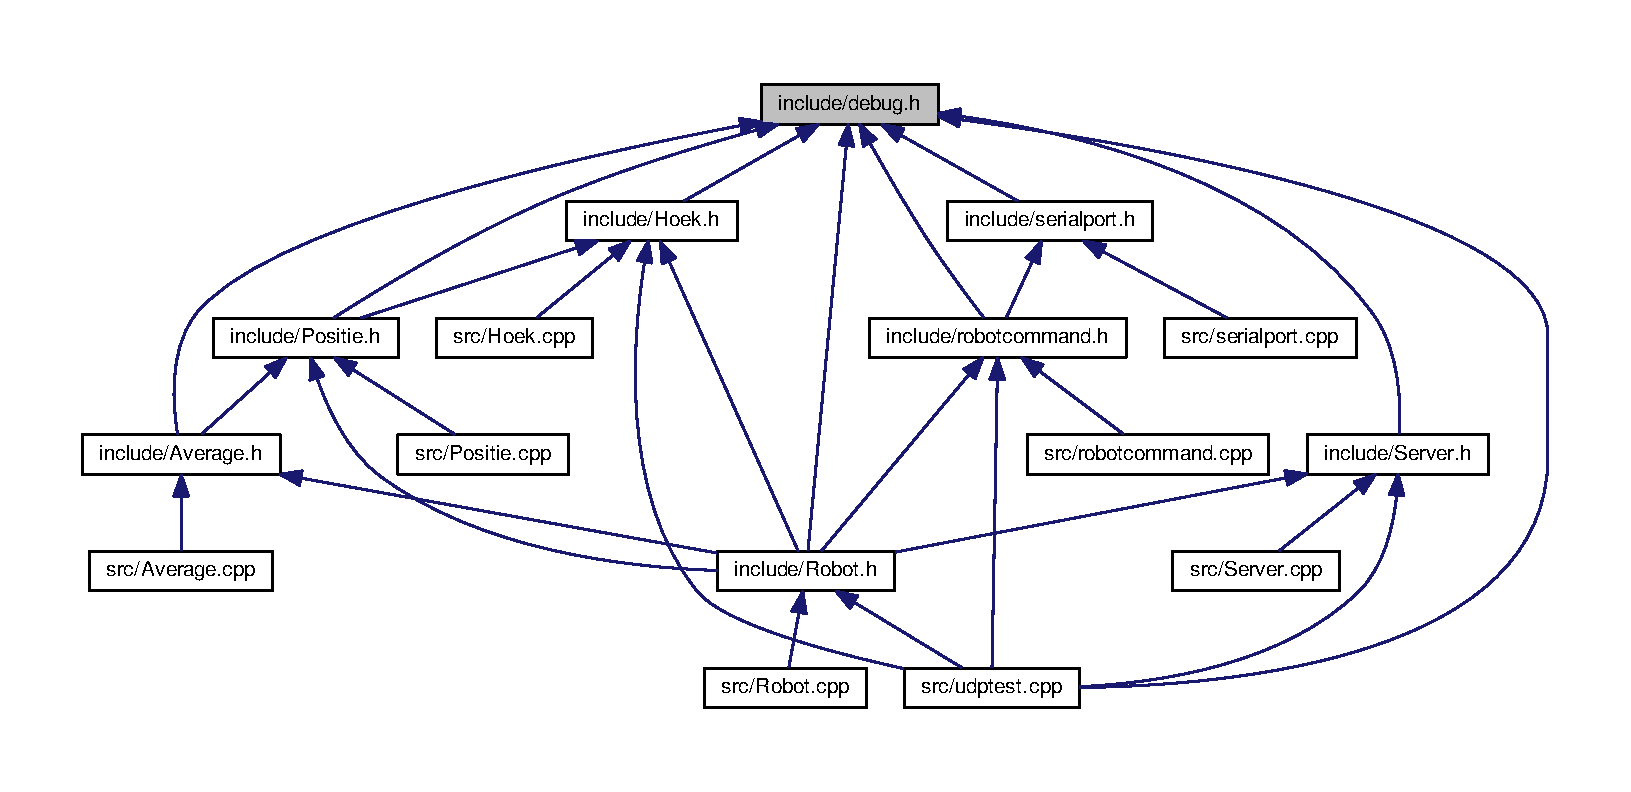
\includegraphics[width=350pt]{debug_8h__dep__incl}
\end{center}
\end{figure}

\hypertarget{Hoek_8h}{\section{include/\-Hoek.h File Reference}
\label{Hoek_8h}\index{include/\-Hoek.\-h@{include/\-Hoek.\-h}}
}
{\ttfamily \#include $<$iostream$>$}\\*
{\ttfamily \#include $<$stdlib.\-h$>$}\\*
{\ttfamily \#include $<$math.\-h$>$}\\*
{\ttfamily \#include \char`\"{}debug.\-h\char`\"{}}\\*
Include dependency graph for Hoek.\-h\-:
\nopagebreak
\begin{figure}[H]
\begin{center}
\leavevmode
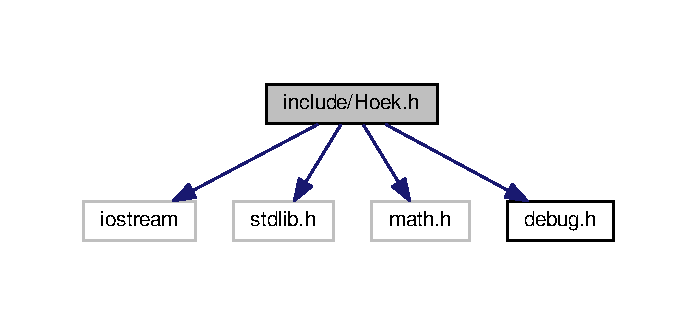
\includegraphics[width=334pt]{Hoek_8h__incl}
\end{center}
\end{figure}
This graph shows which files directly or indirectly include this file\-:
\nopagebreak
\begin{figure}[H]
\begin{center}
\leavevmode
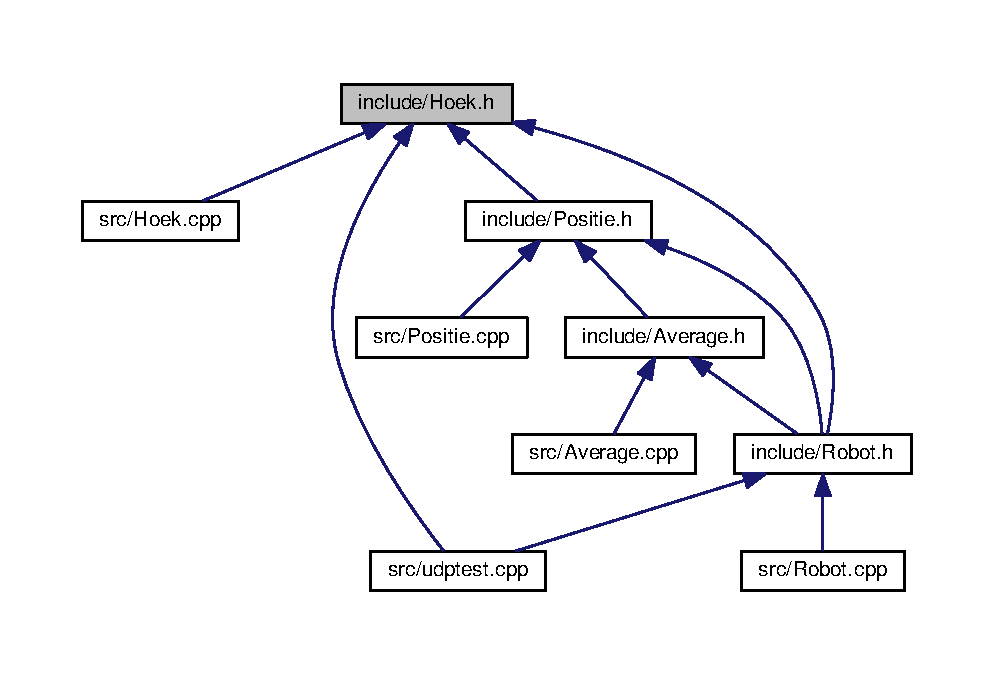
\includegraphics[width=350pt]{Hoek_8h__dep__incl}
\end{center}
\end{figure}
\subsection*{Classes}
\begin{DoxyCompactItemize}
\item 
class \hyperlink{classHoek}{Hoek}
\end{DoxyCompactItemize}
\subsection*{Macros}
\begin{DoxyCompactItemize}
\item 
\#define \hyperlink{Hoek_8h_a598a3330b3c21701223ee0ca14316eca}{P\-I}~3.\-14159265
\item 
\#define \hyperlink{Hoek_8h_a7e49c0004749dd2461e791b4c4a97895}{M\-A\-X\-S\-P\-E\-E\-D}~100
\item 
\#define \hyperlink{Hoek_8h_a5521c82effd93707c3a8f7420ba5881c}{M\-I\-N\-S\-P\-E\-E\-D}~50
\item 
\#define \hyperlink{Hoek_8h_af0230fae7fa772bcbec7c50fba92afa8}{T\-R\-E\-S\-L\-O\-W}~3
\end{DoxyCompactItemize}


\subsection{Macro Definition Documentation}
\hypertarget{Hoek_8h_a7e49c0004749dd2461e791b4c4a97895}{\index{Hoek.\-h@{Hoek.\-h}!M\-A\-X\-S\-P\-E\-E\-D@{M\-A\-X\-S\-P\-E\-E\-D}}
\index{M\-A\-X\-S\-P\-E\-E\-D@{M\-A\-X\-S\-P\-E\-E\-D}!Hoek.h@{Hoek.\-h}}
\subsubsection[{M\-A\-X\-S\-P\-E\-E\-D}]{\setlength{\rightskip}{0pt plus 5cm}\#define M\-A\-X\-S\-P\-E\-E\-D~100}}\label{Hoek_8h_a7e49c0004749dd2461e791b4c4a97895}
\hypertarget{Hoek_8h_a5521c82effd93707c3a8f7420ba5881c}{\index{Hoek.\-h@{Hoek.\-h}!M\-I\-N\-S\-P\-E\-E\-D@{M\-I\-N\-S\-P\-E\-E\-D}}
\index{M\-I\-N\-S\-P\-E\-E\-D@{M\-I\-N\-S\-P\-E\-E\-D}!Hoek.h@{Hoek.\-h}}
\subsubsection[{M\-I\-N\-S\-P\-E\-E\-D}]{\setlength{\rightskip}{0pt plus 5cm}\#define M\-I\-N\-S\-P\-E\-E\-D~50}}\label{Hoek_8h_a5521c82effd93707c3a8f7420ba5881c}
\hypertarget{Hoek_8h_a598a3330b3c21701223ee0ca14316eca}{\index{Hoek.\-h@{Hoek.\-h}!P\-I@{P\-I}}
\index{P\-I@{P\-I}!Hoek.h@{Hoek.\-h}}
\subsubsection[{P\-I}]{\setlength{\rightskip}{0pt plus 5cm}\#define P\-I~3.\-14159265}}\label{Hoek_8h_a598a3330b3c21701223ee0ca14316eca}
\hypertarget{Hoek_8h_af0230fae7fa772bcbec7c50fba92afa8}{\index{Hoek.\-h@{Hoek.\-h}!T\-R\-E\-S\-L\-O\-W@{T\-R\-E\-S\-L\-O\-W}}
\index{T\-R\-E\-S\-L\-O\-W@{T\-R\-E\-S\-L\-O\-W}!Hoek.h@{Hoek.\-h}}
\subsubsection[{T\-R\-E\-S\-L\-O\-W}]{\setlength{\rightskip}{0pt plus 5cm}\#define T\-R\-E\-S\-L\-O\-W~3}}\label{Hoek_8h_af0230fae7fa772bcbec7c50fba92afa8}

\hypertarget{Package_8h}{\section{include/\-Package.h File Reference}
\label{Package_8h}\index{include/\-Package.\-h@{include/\-Package.\-h}}
}
This graph shows which files directly or indirectly include this file\-:
\nopagebreak
\begin{figure}[H]
\begin{center}
\leavevmode
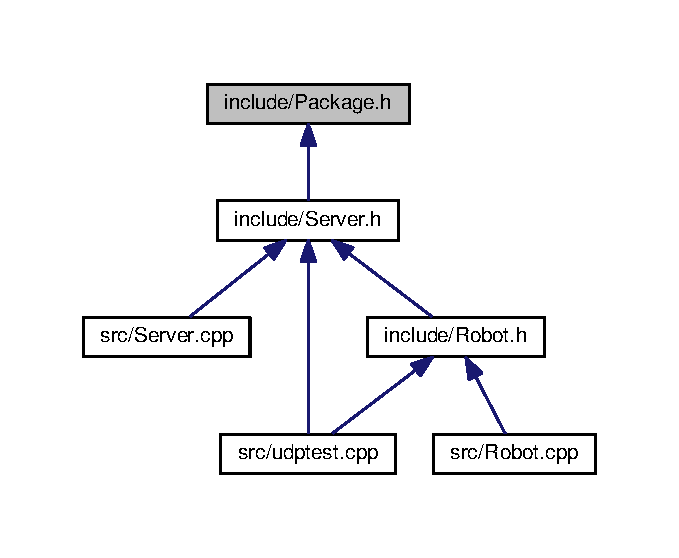
\includegraphics[width=326pt]{Package_8h__dep__incl}
\end{center}
\end{figure}
\subsection*{Classes}
\begin{DoxyCompactItemize}
\item 
struct \hyperlink{structInfo}{Info}
\item 
struct \hyperlink{structUdp__header}{Udp\-\_\-header}
\item 
struct \hyperlink{structUdp__package}{Udp\-\_\-package}
\item 
struct \hyperlink{structPackage}{Package}
\end{DoxyCompactItemize}
\subsection*{Typedefs}
\begin{DoxyCompactItemize}
\item 
typedef struct \hyperlink{structInfo}{Info} \hyperlink{Package_8h_a94af3b57cd50d5de0619fe73dee13795}{Info}
\item 
typedef struct \hyperlink{structUdp__header}{Udp\-\_\-header} \hyperlink{Package_8h_a489a5866dfc8c2b6b3d6ae5b5a902b2c}{Udp\-\_\-header}
\item 
typedef struct \hyperlink{structUdp__package}{Udp\-\_\-package} \hyperlink{Package_8h_ac9cc0e44c001fd515c3a9e2797d2e481}{Udp\-\_\-package}
\item 
typedef struct \hyperlink{structPackage}{Package} \hyperlink{Package_8h_a00a8f77e4db7c79099e180f97aedf284}{Package}
\end{DoxyCompactItemize}


\subsection{Typedef Documentation}
\hypertarget{Package_8h_a94af3b57cd50d5de0619fe73dee13795}{\index{Package.\-h@{Package.\-h}!Info@{Info}}
\index{Info@{Info}!Package.h@{Package.\-h}}
\subsubsection[{Info}]{\setlength{\rightskip}{0pt plus 5cm}typedef struct {\bf Info}  {\bf Info}}}\label{Package_8h_a94af3b57cd50d5de0619fe73dee13795}
\hypertarget{Package_8h_a00a8f77e4db7c79099e180f97aedf284}{\index{Package.\-h@{Package.\-h}!Package@{Package}}
\index{Package@{Package}!Package.h@{Package.\-h}}
\subsubsection[{Package}]{\setlength{\rightskip}{0pt plus 5cm}typedef struct {\bf Package}  {\bf Package}}}\label{Package_8h_a00a8f77e4db7c79099e180f97aedf284}
\hypertarget{Package_8h_a489a5866dfc8c2b6b3d6ae5b5a902b2c}{\index{Package.\-h@{Package.\-h}!Udp\-\_\-header@{Udp\-\_\-header}}
\index{Udp\-\_\-header@{Udp\-\_\-header}!Package.h@{Package.\-h}}
\subsubsection[{Udp\-\_\-header}]{\setlength{\rightskip}{0pt plus 5cm}typedef struct {\bf Udp\-\_\-header}  {\bf Udp\-\_\-header}}}\label{Package_8h_a489a5866dfc8c2b6b3d6ae5b5a902b2c}
\hypertarget{Package_8h_ac9cc0e44c001fd515c3a9e2797d2e481}{\index{Package.\-h@{Package.\-h}!Udp\-\_\-package@{Udp\-\_\-package}}
\index{Udp\-\_\-package@{Udp\-\_\-package}!Package.h@{Package.\-h}}
\subsubsection[{Udp\-\_\-package}]{\setlength{\rightskip}{0pt plus 5cm}typedef struct {\bf Udp\-\_\-package}  {\bf Udp\-\_\-package}}}\label{Package_8h_ac9cc0e44c001fd515c3a9e2797d2e481}

\hypertarget{Positie_8h}{\section{include/\-Positie.h File Reference}
\label{Positie_8h}\index{include/\-Positie.\-h@{include/\-Positie.\-h}}
}
{\ttfamily \#include \char`\"{}debug.\-h\char`\"{}}\\*
{\ttfamily \#include \char`\"{}Hoek.\-h\char`\"{}}\\*
Include dependency graph for Positie.\-h\-:
\nopagebreak
\begin{figure}[H]
\begin{center}
\leavevmode
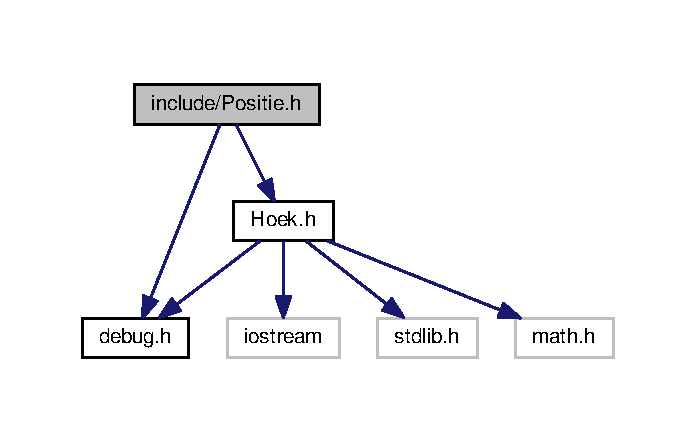
\includegraphics[width=334pt]{Positie_8h__incl}
\end{center}
\end{figure}
This graph shows which files directly or indirectly include this file\-:
\nopagebreak
\begin{figure}[H]
\begin{center}
\leavevmode
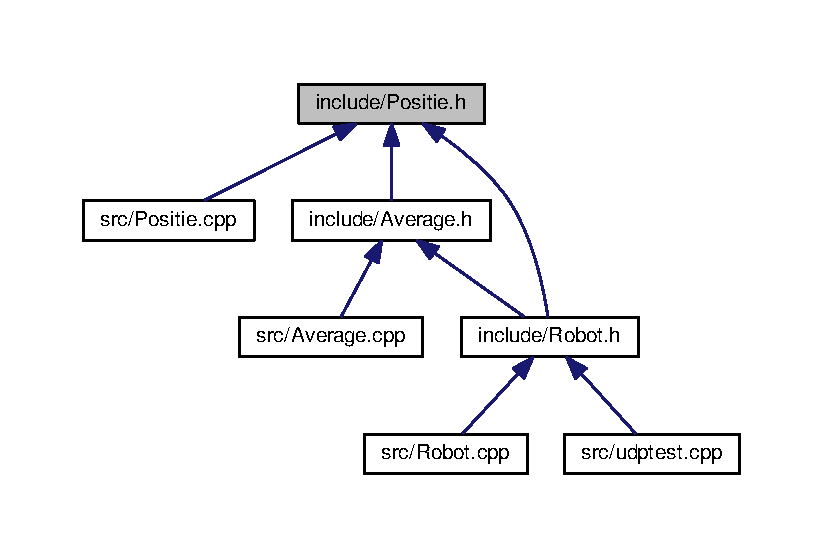
\includegraphics[width=350pt]{Positie_8h__dep__incl}
\end{center}
\end{figure}
\subsection*{Classes}
\begin{DoxyCompactItemize}
\item 
class \hyperlink{classPositie}{Positie}
\end{DoxyCompactItemize}

\hypertarget{Robot_8h}{\section{include/\-Robot.h File Reference}
\label{Robot_8h}\index{include/\-Robot.\-h@{include/\-Robot.\-h}}
}
{\ttfamily \#include $<$string$>$}\\*
{\ttfamily \#include \char`\"{}debug.\-h\char`\"{}}\\*
{\ttfamily \#include \char`\"{}Positie.\-h\char`\"{}}\\*
{\ttfamily \#include \char`\"{}Server.\-h\char`\"{}}\\*
{\ttfamily \#include \char`\"{}robotcommand.\-h\char`\"{}}\\*
{\ttfamily \#include \char`\"{}Hoek.\-h\char`\"{}}\\*
{\ttfamily \#include \char`\"{}Average.\-h\char`\"{}}\\*
Include dependency graph for Robot.\-h\-:
\nopagebreak
\begin{figure}[H]
\begin{center}
\leavevmode
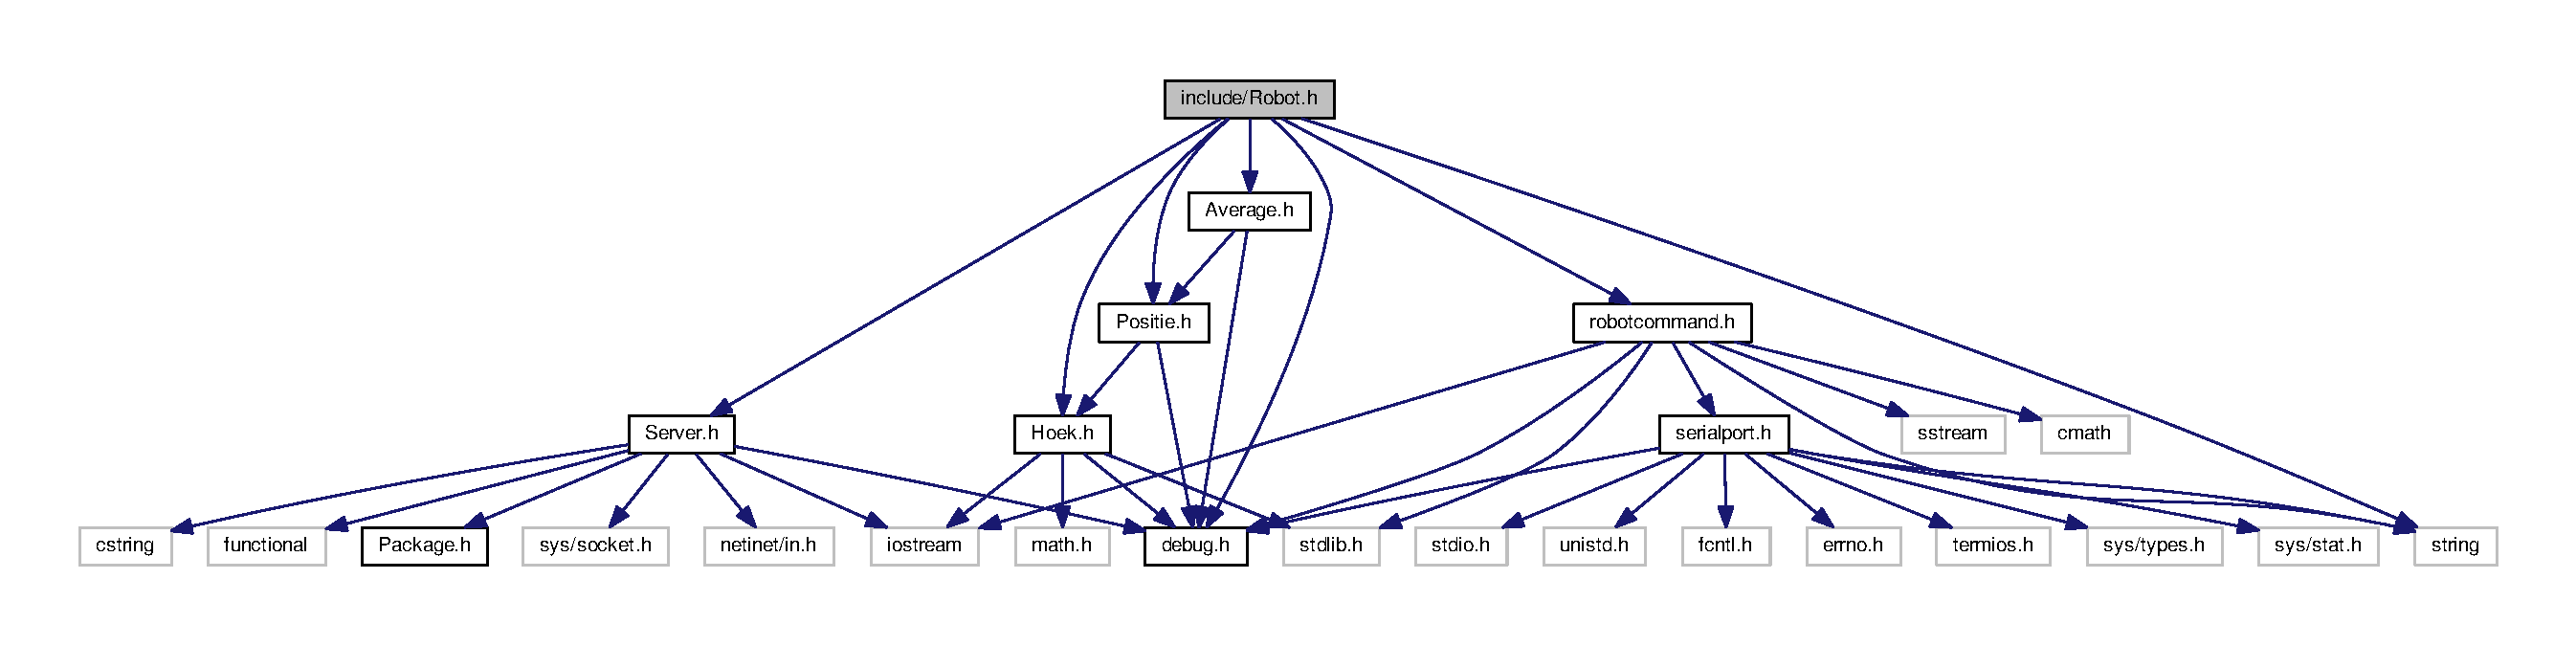
\includegraphics[width=350pt]{Robot_8h__incl}
\end{center}
\end{figure}
This graph shows which files directly or indirectly include this file\-:
\nopagebreak
\begin{figure}[H]
\begin{center}
\leavevmode
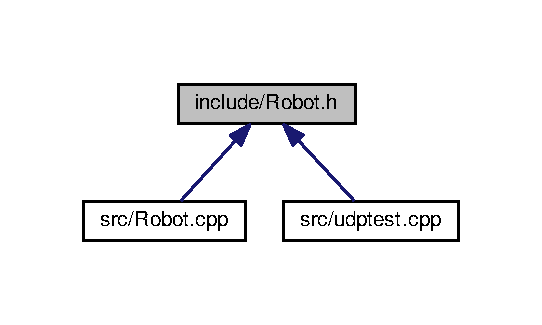
\includegraphics[width=260pt]{Robot_8h__dep__incl}
\end{center}
\end{figure}
\subsection*{Classes}
\begin{DoxyCompactItemize}
\item 
class \hyperlink{classRobot}{Robot}
\end{DoxyCompactItemize}

\hypertarget{robotcommand_8h}{\section{include/robotcommand.h File Reference}
\label{robotcommand_8h}\index{include/robotcommand.\-h@{include/robotcommand.\-h}}
}
{\ttfamily \#include $<$iostream$>$}\\*
{\ttfamily \#include $<$string$>$}\\*
{\ttfamily \#include $<$sstream$>$}\\*
{\ttfamily \#include $<$cmath$>$}\\*
{\ttfamily \#include $<$stdlib.\-h$>$}\\*
{\ttfamily \#include \char`\"{}debug.\-h\char`\"{}}\\*
{\ttfamily \#include \char`\"{}serialport.\-h\char`\"{}}\\*
Include dependency graph for robotcommand.\-h\-:
\nopagebreak
\begin{figure}[H]
\begin{center}
\leavevmode
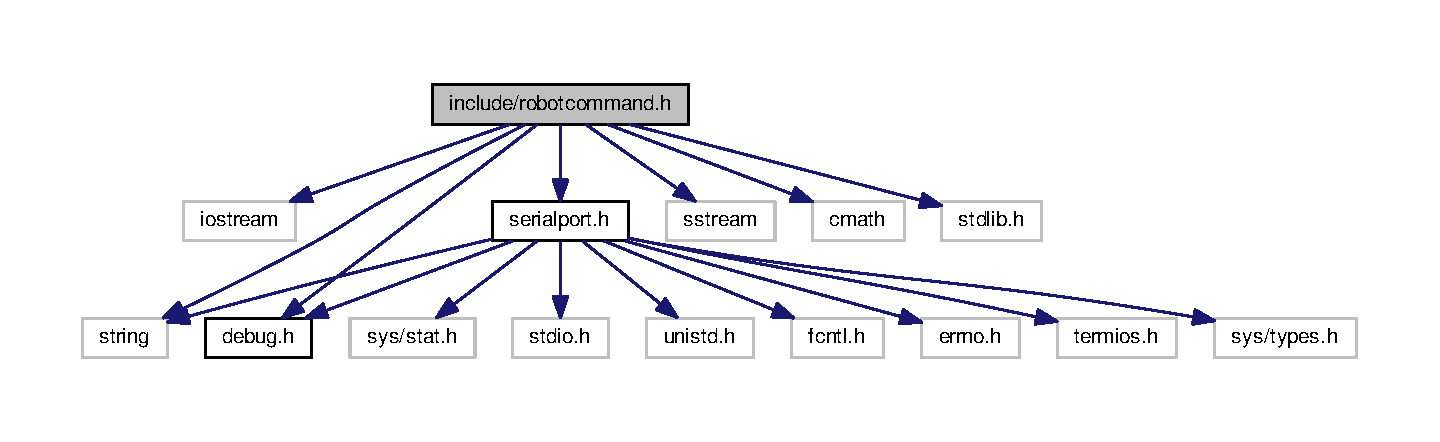
\includegraphics[width=350pt]{robotcommand_8h__incl}
\end{center}
\end{figure}
This graph shows which files directly or indirectly include this file\-:
\nopagebreak
\begin{figure}[H]
\begin{center}
\leavevmode
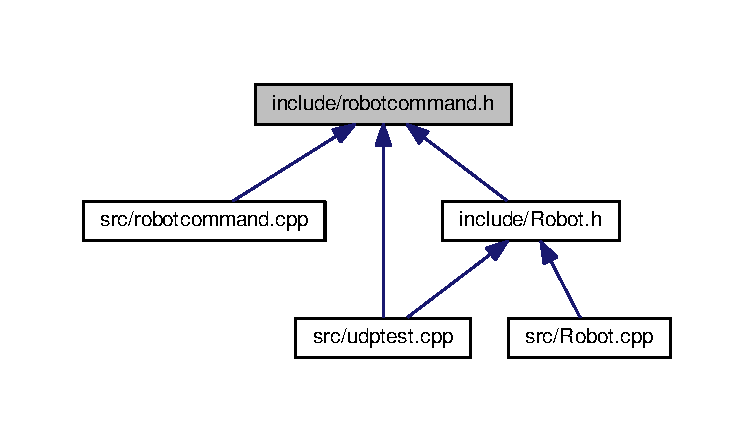
\includegraphics[width=350pt]{robotcommand_8h__dep__incl}
\end{center}
\end{figure}
\subsection*{Classes}
\begin{DoxyCompactItemize}
\item 
class \hyperlink{classrobotcommand}{robotcommand}
\end{DoxyCompactItemize}
\subsection*{Macros}
\begin{DoxyCompactItemize}
\item 
\#define \hyperlink{robotcommand_8h_a68f19c90ab1da05d928e40069ff5abd5}{T\-U\-R\-N\-S\-P\-E\-E\-D}~100
\item 
\#define \hyperlink{robotcommand_8h_a305e4f58554eb443401652c5b4d6888a}{D\-E\-G\-M\-U\-L\-T}~100
\item 
\#define \hyperlink{robotcommand_8h_acc64290a85dbe333a83a07f869c0a91b}{D\-E\-G\-P\-E\-R\-S\-E\-C}~4500
\item 
\#define \hyperlink{robotcommand_8h_acd526f11ce51532b8187f63bac77d87b}{S\-E\-R\-I\-A\-L\-P\-O\-R\-T}~\char`\"{}/dev/tty\-U\-S\-B0\char`\"{}
\end{DoxyCompactItemize}


\subsection{Macro Definition Documentation}
\hypertarget{robotcommand_8h_a305e4f58554eb443401652c5b4d6888a}{\index{robotcommand.\-h@{robotcommand.\-h}!D\-E\-G\-M\-U\-L\-T@{D\-E\-G\-M\-U\-L\-T}}
\index{D\-E\-G\-M\-U\-L\-T@{D\-E\-G\-M\-U\-L\-T}!robotcommand.h@{robotcommand.\-h}}
\subsubsection[{D\-E\-G\-M\-U\-L\-T}]{\setlength{\rightskip}{0pt plus 5cm}\#define D\-E\-G\-M\-U\-L\-T~100}}\label{robotcommand_8h_a305e4f58554eb443401652c5b4d6888a}
\hypertarget{robotcommand_8h_acc64290a85dbe333a83a07f869c0a91b}{\index{robotcommand.\-h@{robotcommand.\-h}!D\-E\-G\-P\-E\-R\-S\-E\-C@{D\-E\-G\-P\-E\-R\-S\-E\-C}}
\index{D\-E\-G\-P\-E\-R\-S\-E\-C@{D\-E\-G\-P\-E\-R\-S\-E\-C}!robotcommand.h@{robotcommand.\-h}}
\subsubsection[{D\-E\-G\-P\-E\-R\-S\-E\-C}]{\setlength{\rightskip}{0pt plus 5cm}\#define D\-E\-G\-P\-E\-R\-S\-E\-C~4500}}\label{robotcommand_8h_acc64290a85dbe333a83a07f869c0a91b}
\hypertarget{robotcommand_8h_acd526f11ce51532b8187f63bac77d87b}{\index{robotcommand.\-h@{robotcommand.\-h}!S\-E\-R\-I\-A\-L\-P\-O\-R\-T@{S\-E\-R\-I\-A\-L\-P\-O\-R\-T}}
\index{S\-E\-R\-I\-A\-L\-P\-O\-R\-T@{S\-E\-R\-I\-A\-L\-P\-O\-R\-T}!robotcommand.h@{robotcommand.\-h}}
\subsubsection[{S\-E\-R\-I\-A\-L\-P\-O\-R\-T}]{\setlength{\rightskip}{0pt plus 5cm}\#define S\-E\-R\-I\-A\-L\-P\-O\-R\-T~\char`\"{}/dev/tty\-U\-S\-B0\char`\"{}}}\label{robotcommand_8h_acd526f11ce51532b8187f63bac77d87b}
\hypertarget{robotcommand_8h_a68f19c90ab1da05d928e40069ff5abd5}{\index{robotcommand.\-h@{robotcommand.\-h}!T\-U\-R\-N\-S\-P\-E\-E\-D@{T\-U\-R\-N\-S\-P\-E\-E\-D}}
\index{T\-U\-R\-N\-S\-P\-E\-E\-D@{T\-U\-R\-N\-S\-P\-E\-E\-D}!robotcommand.h@{robotcommand.\-h}}
\subsubsection[{T\-U\-R\-N\-S\-P\-E\-E\-D}]{\setlength{\rightskip}{0pt plus 5cm}\#define T\-U\-R\-N\-S\-P\-E\-E\-D~100}}\label{robotcommand_8h_a68f19c90ab1da05d928e40069ff5abd5}

\hypertarget{serialport_8h}{\section{include/serialport.h File Reference}
\label{serialport_8h}\index{include/serialport.\-h@{include/serialport.\-h}}
}
{\ttfamily \#include $<$stdio.\-h$>$}\\*
{\ttfamily \#include $<$string$>$}\\*
{\ttfamily \#include $<$unistd.\-h$>$}\\*
{\ttfamily \#include $<$fcntl.\-h$>$}\\*
{\ttfamily \#include $<$errno.\-h$>$}\\*
{\ttfamily \#include $<$termios.\-h$>$}\\*
{\ttfamily \#include $<$sys/types.\-h$>$}\\*
{\ttfamily \#include $<$sys/stat.\-h$>$}\\*
{\ttfamily \#include \char`\"{}debug.\-h\char`\"{}}\\*
Include dependency graph for serialport.\-h\-:
\nopagebreak
\begin{figure}[H]
\begin{center}
\leavevmode
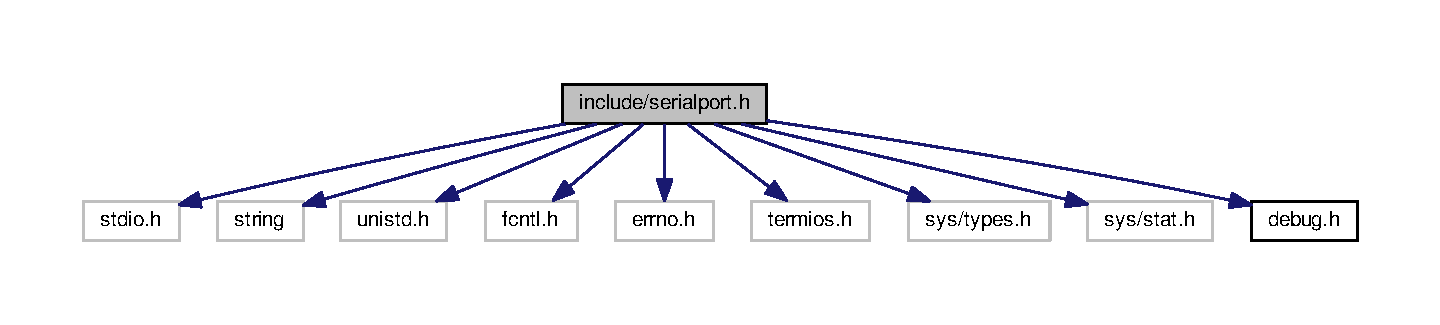
\includegraphics[width=350pt]{serialport_8h__incl}
\end{center}
\end{figure}
This graph shows which files directly or indirectly include this file\-:
\nopagebreak
\begin{figure}[H]
\begin{center}
\leavevmode
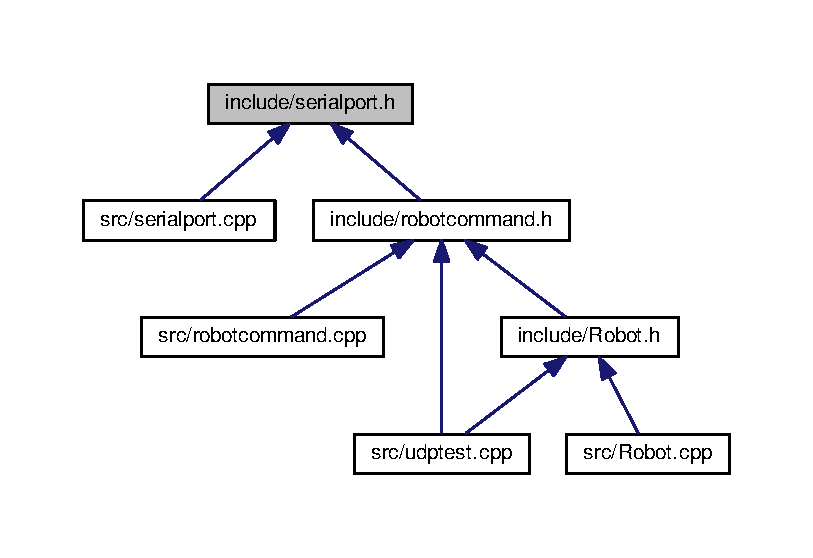
\includegraphics[width=350pt]{serialport_8h__dep__incl}
\end{center}
\end{figure}
\subsection*{Classes}
\begin{DoxyCompactItemize}
\item 
class \hyperlink{classserialport}{serialport}
\end{DoxyCompactItemize}
\subsection*{Macros}
\begin{DoxyCompactItemize}
\item 
\#define \hyperlink{serialport_8h_a614217d263be1fb1a5f76e2ff7be19a2}{P\-O\-R\-T}~\char`\"{}/dev/tty\-U\-S\-B0\char`\"{}
\item 
\#define \hyperlink{serialport_8h_a155a9a6160c909e29d95e7c75b79612a}{D\-A\-T\-A\-B\-I\-T\-S}~8
\item 
\#define \hyperlink{serialport_8h_aa5d0b84610803adad91c781c7a51be82}{S\-T\-O\-P\-B\-I\-T\-S}~1
\item 
\#define \hyperlink{serialport_8h_aff1f07741fbe1f53f46098687f0a05e2}{F\-L\-O\-W\-C\-O\-N\-T\-R\-O\-L}~0
\item 
\#define \hyperlink{serialport_8h_ac3d144aa01e765a1fae62ab5491c7cc1}{\-\_\-\-P\-O\-S\-I\-X\-\_\-\-S\-O\-U\-R\-C\-E}~1 /$\ast$ P\-O\-S\-I\-X compliant source $\ast$/
\item 
\#define \hyperlink{serialport_8h_a6f63eb988b0b1344d3a4a00adca2429b}{S\-E\-R\-I\-A\-L\-\_\-\-B\-U\-F\-\_\-\-L\-E\-N}~100
\item 
\#define \hyperlink{serialport_8h_aa93f0eb578d23995850d61f7d61c55c1}{F\-A\-L\-S\-E}~0
\item 
\#define \hyperlink{serialport_8h_aa8cecfc5c5c054d2875c03e77b7be15d}{T\-R\-U\-E}~1
\end{DoxyCompactItemize}


\subsection{Macro Definition Documentation}
\hypertarget{serialport_8h_ac3d144aa01e765a1fae62ab5491c7cc1}{\index{serialport.\-h@{serialport.\-h}!\-\_\-\-P\-O\-S\-I\-X\-\_\-\-S\-O\-U\-R\-C\-E@{\-\_\-\-P\-O\-S\-I\-X\-\_\-\-S\-O\-U\-R\-C\-E}}
\index{\-\_\-\-P\-O\-S\-I\-X\-\_\-\-S\-O\-U\-R\-C\-E@{\-\_\-\-P\-O\-S\-I\-X\-\_\-\-S\-O\-U\-R\-C\-E}!serialport.h@{serialport.\-h}}
\subsubsection[{\-\_\-\-P\-O\-S\-I\-X\-\_\-\-S\-O\-U\-R\-C\-E}]{\setlength{\rightskip}{0pt plus 5cm}\#define \-\_\-\-P\-O\-S\-I\-X\-\_\-\-S\-O\-U\-R\-C\-E~1 /$\ast$ P\-O\-S\-I\-X compliant source $\ast$/}}\label{serialport_8h_ac3d144aa01e765a1fae62ab5491c7cc1}
\hypertarget{serialport_8h_a155a9a6160c909e29d95e7c75b79612a}{\index{serialport.\-h@{serialport.\-h}!D\-A\-T\-A\-B\-I\-T\-S@{D\-A\-T\-A\-B\-I\-T\-S}}
\index{D\-A\-T\-A\-B\-I\-T\-S@{D\-A\-T\-A\-B\-I\-T\-S}!serialport.h@{serialport.\-h}}
\subsubsection[{D\-A\-T\-A\-B\-I\-T\-S}]{\setlength{\rightskip}{0pt plus 5cm}\#define D\-A\-T\-A\-B\-I\-T\-S~8}}\label{serialport_8h_a155a9a6160c909e29d95e7c75b79612a}
\hypertarget{serialport_8h_aa93f0eb578d23995850d61f7d61c55c1}{\index{serialport.\-h@{serialport.\-h}!F\-A\-L\-S\-E@{F\-A\-L\-S\-E}}
\index{F\-A\-L\-S\-E@{F\-A\-L\-S\-E}!serialport.h@{serialport.\-h}}
\subsubsection[{F\-A\-L\-S\-E}]{\setlength{\rightskip}{0pt plus 5cm}\#define F\-A\-L\-S\-E~0}}\label{serialport_8h_aa93f0eb578d23995850d61f7d61c55c1}
\hypertarget{serialport_8h_aff1f07741fbe1f53f46098687f0a05e2}{\index{serialport.\-h@{serialport.\-h}!F\-L\-O\-W\-C\-O\-N\-T\-R\-O\-L@{F\-L\-O\-W\-C\-O\-N\-T\-R\-O\-L}}
\index{F\-L\-O\-W\-C\-O\-N\-T\-R\-O\-L@{F\-L\-O\-W\-C\-O\-N\-T\-R\-O\-L}!serialport.h@{serialport.\-h}}
\subsubsection[{F\-L\-O\-W\-C\-O\-N\-T\-R\-O\-L}]{\setlength{\rightskip}{0pt plus 5cm}\#define F\-L\-O\-W\-C\-O\-N\-T\-R\-O\-L~0}}\label{serialport_8h_aff1f07741fbe1f53f46098687f0a05e2}
\hypertarget{serialport_8h_a614217d263be1fb1a5f76e2ff7be19a2}{\index{serialport.\-h@{serialport.\-h}!P\-O\-R\-T@{P\-O\-R\-T}}
\index{P\-O\-R\-T@{P\-O\-R\-T}!serialport.h@{serialport.\-h}}
\subsubsection[{P\-O\-R\-T}]{\setlength{\rightskip}{0pt plus 5cm}\#define P\-O\-R\-T~\char`\"{}/dev/tty\-U\-S\-B0\char`\"{}}}\label{serialport_8h_a614217d263be1fb1a5f76e2ff7be19a2}
\hypertarget{serialport_8h_a6f63eb988b0b1344d3a4a00adca2429b}{\index{serialport.\-h@{serialport.\-h}!S\-E\-R\-I\-A\-L\-\_\-\-B\-U\-F\-\_\-\-L\-E\-N@{S\-E\-R\-I\-A\-L\-\_\-\-B\-U\-F\-\_\-\-L\-E\-N}}
\index{S\-E\-R\-I\-A\-L\-\_\-\-B\-U\-F\-\_\-\-L\-E\-N@{S\-E\-R\-I\-A\-L\-\_\-\-B\-U\-F\-\_\-\-L\-E\-N}!serialport.h@{serialport.\-h}}
\subsubsection[{S\-E\-R\-I\-A\-L\-\_\-\-B\-U\-F\-\_\-\-L\-E\-N}]{\setlength{\rightskip}{0pt plus 5cm}\#define S\-E\-R\-I\-A\-L\-\_\-\-B\-U\-F\-\_\-\-L\-E\-N~100}}\label{serialport_8h_a6f63eb988b0b1344d3a4a00adca2429b}
\hypertarget{serialport_8h_aa5d0b84610803adad91c781c7a51be82}{\index{serialport.\-h@{serialport.\-h}!S\-T\-O\-P\-B\-I\-T\-S@{S\-T\-O\-P\-B\-I\-T\-S}}
\index{S\-T\-O\-P\-B\-I\-T\-S@{S\-T\-O\-P\-B\-I\-T\-S}!serialport.h@{serialport.\-h}}
\subsubsection[{S\-T\-O\-P\-B\-I\-T\-S}]{\setlength{\rightskip}{0pt plus 5cm}\#define S\-T\-O\-P\-B\-I\-T\-S~1}}\label{serialport_8h_aa5d0b84610803adad91c781c7a51be82}
\hypertarget{serialport_8h_aa8cecfc5c5c054d2875c03e77b7be15d}{\index{serialport.\-h@{serialport.\-h}!T\-R\-U\-E@{T\-R\-U\-E}}
\index{T\-R\-U\-E@{T\-R\-U\-E}!serialport.h@{serialport.\-h}}
\subsubsection[{T\-R\-U\-E}]{\setlength{\rightskip}{0pt plus 5cm}\#define T\-R\-U\-E~1}}\label{serialport_8h_aa8cecfc5c5c054d2875c03e77b7be15d}

\hypertarget{Server_8h}{\section{include/\-Server.h File Reference}
\label{Server_8h}\index{include/\-Server.\-h@{include/\-Server.\-h}}
}
{\ttfamily \#include $<$sys/socket.\-h$>$}\\*
{\ttfamily \#include $<$netinet/in.\-h$>$}\\*
{\ttfamily \#include $<$iostream$>$}\\*
{\ttfamily \#include $<$cstring$>$}\\*
{\ttfamily \#include $<$functional$>$}\\*
{\ttfamily \#include \char`\"{}debug.\-h\char`\"{}}\\*
{\ttfamily \#include \char`\"{}Package.\-h\char`\"{}}\\*
Include dependency graph for Server.\-h\-:
\nopagebreak
\begin{figure}[H]
\begin{center}
\leavevmode
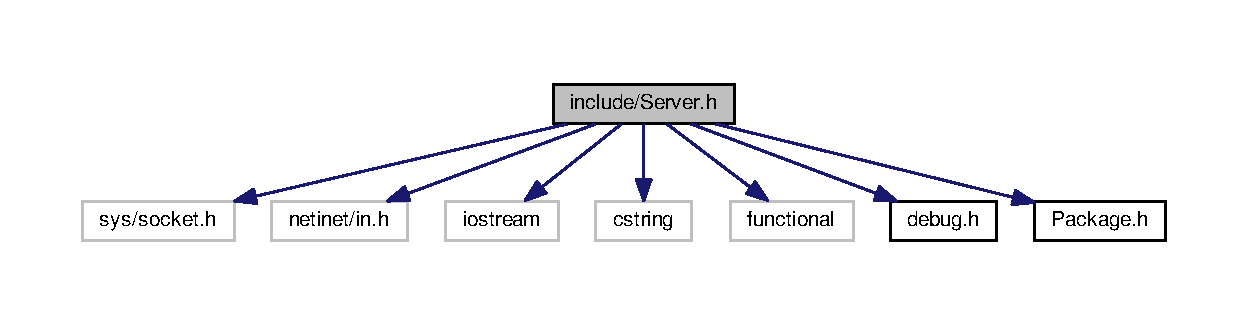
\includegraphics[width=350pt]{Server_8h__incl}
\end{center}
\end{figure}
This graph shows which files directly or indirectly include this file\-:
\nopagebreak
\begin{figure}[H]
\begin{center}
\leavevmode
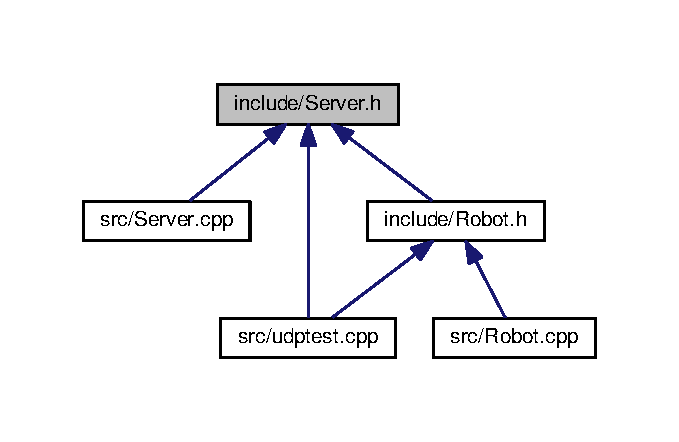
\includegraphics[width=326pt]{Server_8h__dep__incl}
\end{center}
\end{figure}
\subsection*{Classes}
\begin{DoxyCompactItemize}
\item 
class \hyperlink{classServer}{Server}
\end{DoxyCompactItemize}
\subsection*{Macros}
\begin{DoxyCompactItemize}
\item 
\#define \hyperlink{Server_8h_ab52a72e164e6995d7693a24dc3c43472}{S\-T\-A\-N\-D\-A\-A\-R\-D\-G\-R\-O\-E\-P}~'b'
\item 
\#define \hyperlink{Server_8h_aba1a0da5373c381e0ad6481f8333c08a}{S\-T\-A\-N\-D\-A\-A\-R\-D\-P\-O\-O\-R\-T}~3200
\end{DoxyCompactItemize}


\subsection{Macro Definition Documentation}
\hypertarget{Server_8h_ab52a72e164e6995d7693a24dc3c43472}{\index{Server.\-h@{Server.\-h}!S\-T\-A\-N\-D\-A\-A\-R\-D\-G\-R\-O\-E\-P@{S\-T\-A\-N\-D\-A\-A\-R\-D\-G\-R\-O\-E\-P}}
\index{S\-T\-A\-N\-D\-A\-A\-R\-D\-G\-R\-O\-E\-P@{S\-T\-A\-N\-D\-A\-A\-R\-D\-G\-R\-O\-E\-P}!Server.h@{Server.\-h}}
\subsubsection[{S\-T\-A\-N\-D\-A\-A\-R\-D\-G\-R\-O\-E\-P}]{\setlength{\rightskip}{0pt plus 5cm}\#define S\-T\-A\-N\-D\-A\-A\-R\-D\-G\-R\-O\-E\-P~'b'}}\label{Server_8h_ab52a72e164e6995d7693a24dc3c43472}
\hypertarget{Server_8h_aba1a0da5373c381e0ad6481f8333c08a}{\index{Server.\-h@{Server.\-h}!S\-T\-A\-N\-D\-A\-A\-R\-D\-P\-O\-O\-R\-T@{S\-T\-A\-N\-D\-A\-A\-R\-D\-P\-O\-O\-R\-T}}
\index{S\-T\-A\-N\-D\-A\-A\-R\-D\-P\-O\-O\-R\-T@{S\-T\-A\-N\-D\-A\-A\-R\-D\-P\-O\-O\-R\-T}!Server.h@{Server.\-h}}
\subsubsection[{S\-T\-A\-N\-D\-A\-A\-R\-D\-P\-O\-O\-R\-T}]{\setlength{\rightskip}{0pt plus 5cm}\#define S\-T\-A\-N\-D\-A\-A\-R\-D\-P\-O\-O\-R\-T~3200}}\label{Server_8h_aba1a0da5373c381e0ad6481f8333c08a}

\hypertarget{Average_8cpp}{\section{src/\-Average.cpp File Reference}
\label{Average_8cpp}\index{src/\-Average.\-cpp@{src/\-Average.\-cpp}}
}
{\ttfamily \#include \char`\"{}Average.\-h\char`\"{}}\\*
Include dependency graph for Average.\-cpp\-:
\nopagebreak
\begin{figure}[H]
\begin{center}
\leavevmode
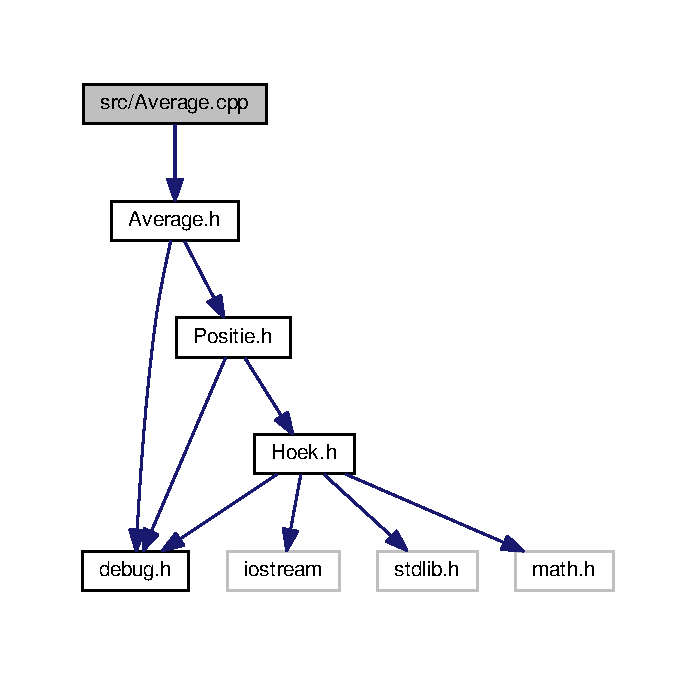
\includegraphics[width=334pt]{Average_8cpp__incl}
\end{center}
\end{figure}

\hypertarget{Hoek_8cpp}{\section{src/\-Hoek.cpp File Reference}
\label{Hoek_8cpp}\index{src/\-Hoek.\-cpp@{src/\-Hoek.\-cpp}}
}
{\ttfamily \#include \char`\"{}Hoek.\-h\char`\"{}}\\*
Include dependency graph for Hoek.\-cpp\-:
\nopagebreak
\begin{figure}[H]
\begin{center}
\leavevmode
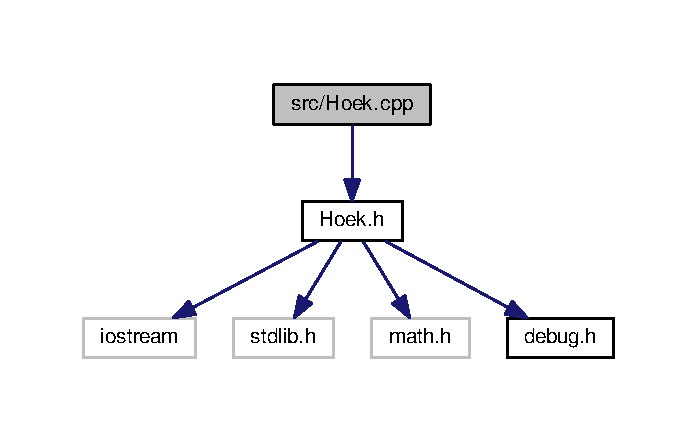
\includegraphics[width=334pt]{Hoek_8cpp__incl}
\end{center}
\end{figure}

\hypertarget{Positie_8cpp}{\section{src/\-Positie.cpp File Reference}
\label{Positie_8cpp}\index{src/\-Positie.\-cpp@{src/\-Positie.\-cpp}}
}
{\ttfamily \#include \char`\"{}Positie.\-h\char`\"{}}\\*
Include dependency graph for Positie.\-cpp\-:
\nopagebreak
\begin{figure}[H]
\begin{center}
\leavevmode
\includegraphics[width=334pt]{Positie_8cpp__incl}
\end{center}
\end{figure}
\subsection*{Macros}
\begin{DoxyCompactItemize}
\item 
\#define \hyperlink{Positie_8cpp_a14f4d979f60a97d89edc64142dd1d96a}{T\-R\-E\-S\-H\-O\-L\-D\-E\-Q\-U\-A\-L}~20
\end{DoxyCompactItemize}


\subsection{Macro Definition Documentation}
\hypertarget{Positie_8cpp_a14f4d979f60a97d89edc64142dd1d96a}{\index{Positie.\-cpp@{Positie.\-cpp}!T\-R\-E\-S\-H\-O\-L\-D\-E\-Q\-U\-A\-L@{T\-R\-E\-S\-H\-O\-L\-D\-E\-Q\-U\-A\-L}}
\index{T\-R\-E\-S\-H\-O\-L\-D\-E\-Q\-U\-A\-L@{T\-R\-E\-S\-H\-O\-L\-D\-E\-Q\-U\-A\-L}!Positie.cpp@{Positie.\-cpp}}
\subsubsection[{T\-R\-E\-S\-H\-O\-L\-D\-E\-Q\-U\-A\-L}]{\setlength{\rightskip}{0pt plus 5cm}\#define T\-R\-E\-S\-H\-O\-L\-D\-E\-Q\-U\-A\-L~20}}\label{Positie_8cpp_a14f4d979f60a97d89edc64142dd1d96a}

\hypertarget{Robot_8cpp}{\section{src/\-Robot.cpp File Reference}
\label{Robot_8cpp}\index{src/\-Robot.\-cpp@{src/\-Robot.\-cpp}}
}
{\ttfamily \#include \char`\"{}Robot.\-h\char`\"{}}\\*
Include dependency graph for Robot.\-cpp\-:
\nopagebreak
\begin{figure}[H]
\begin{center}
\leavevmode
\includegraphics[width=350pt]{Robot_8cpp__incl}
\end{center}
\end{figure}

\hypertarget{robotcommand_8cpp}{\section{src/robotcommand.cpp File Reference}
\label{robotcommand_8cpp}\index{src/robotcommand.\-cpp@{src/robotcommand.\-cpp}}
}
{\ttfamily \#include \char`\"{}robotcommand.\-h\char`\"{}}\\*
Include dependency graph for robotcommand.\-cpp\-:
\nopagebreak
\begin{figure}[H]
\begin{center}
\leavevmode
\includegraphics[width=350pt]{robotcommand_8cpp__incl}
\end{center}
\end{figure}

\hypertarget{serialport_8cpp}{\section{src/serialport.cpp File Reference}
\label{serialport_8cpp}\index{src/serialport.\-cpp@{src/serialport.\-cpp}}
}
{\ttfamily \#include \char`\"{}serialport.\-h\char`\"{}}\\*
{\ttfamily \#include $<$string.\-h$>$}\\*
{\ttfamily \#include $<$iostream$>$}\\*
Include dependency graph for serialport.\-cpp\-:
\nopagebreak
\begin{figure}[H]
\begin{center}
\leavevmode
\includegraphics[width=350pt]{serialport_8cpp__incl}
\end{center}
\end{figure}

\hypertarget{Server_8cpp}{\section{src/\-Server.cpp File Reference}
\label{Server_8cpp}\index{src/\-Server.\-cpp@{src/\-Server.\-cpp}}
}
{\ttfamily \#include \char`\"{}Server.\-h\char`\"{}}\\*
Include dependency graph for Server.\-cpp\-:
\nopagebreak
\begin{figure}[H]
\begin{center}
\leavevmode
\includegraphics[width=350pt]{Server_8cpp__incl}
\end{center}
\end{figure}

\hypertarget{udptest_8cpp}{\section{src/udptest.cpp File Reference}
\label{udptest_8cpp}\index{src/udptest.\-cpp@{src/udptest.\-cpp}}
}
{\ttfamily \#include $<$iostream$>$}\\*
{\ttfamily \#include $<$csignal$>$}\\*
{\ttfamily \#include $<$cstdlib$>$}\\*
{\ttfamily \#include $<$math.\-h$>$}\\*
{\ttfamily \#include $<$unistd.\-h$>$}\\*
{\ttfamily \#include \char`\"{}debug.\-h\char`\"{}}\\*
{\ttfamily \#include \char`\"{}Server.\-h\char`\"{}}\\*
{\ttfamily \#include \char`\"{}Robot.\-h\char`\"{}}\\*
{\ttfamily \#include \char`\"{}Hoek.\-h\char`\"{}}\\*
{\ttfamily \#include \char`\"{}robotcommand.\-h\char`\"{}}\\*
Include dependency graph for udptest.\-cpp\-:
\nopagebreak
\begin{figure}[H]
\begin{center}
\leavevmode
\includegraphics[width=350pt]{udptest_8cpp__incl}
\end{center}
\end{figure}
\subsection*{Macros}
\begin{DoxyCompactItemize}
\item 
\#define \hyperlink{udptest_8cpp_ad04e024503e80de4acff2d4ea711d611}{D\-R\-A\-A\-I\-S\-P\-E\-E\-D\-M\-I\-N}~20
\item 
\#define \hyperlink{udptest_8cpp_ab3ace374e857e47b2bb5005ab5bc6cc9}{D\-R\-A\-A\-I\-S\-P\-E\-E\-D\-M\-A\-X}~40
\item 
\#define \hyperlink{udptest_8cpp_a16bc66c577ce5feda5f142a408c7634a}{G\-R\-O\-T\-E\-A\-F\-S\-T\-A\-N\-D}~70
\item 
\#define \hyperlink{udptest_8cpp_ab6096b33a72e7b43ad4d43ba5c1fd70c}{C\-I\-R\-K\-E\-L\-T\-R\-E\-S\-H\-O\-L\-D\-V\-A\-N\-B\-L\-I\-K}~100
\item 
\#define \hyperlink{udptest_8cpp_aeea05c41d6f5117ad278a01c0960922c}{C\-I\-R\-K\-E\-L\-T\-R\-E\-S\-H\-O\-L\-D\-V\-A\-N\-G\-A\-R\-A\-G\-E}~100
\item 
\#define \hyperlink{udptest_8cpp_adce2989cfd25956296a78dacbeb04264}{A\-F\-S\-T\-A\-N\-D\-T\-R\-E\-S\-H\-O\-L\-D\-B\-L\-I\-K\-J\-E\-R\-O\-B\-O\-T}~45
\item 
\#define \hyperlink{udptest_8cpp_a755b4f232e7b9d14bf5548785ac6cc24}{I\-N\-I\-T\-R\-O\-B\-O\-T}~0
\item 
\#define \hyperlink{udptest_8cpp_af849506c5c84ba63c9bf515fac73e625}{D\-R\-A\-A\-I\-N\-A\-A\-R\-B\-L\-I\-K}~1
\item 
\#define \hyperlink{udptest_8cpp_a0e4bb9102b946b174080cdf975b47af3}{R\-I\-J\-N\-A\-A\-R\-B\-L\-I\-K}~2
\item 
\#define \hyperlink{udptest_8cpp_a7ce3eb237ae6e9aba9674298bdebc2ef}{B\-I\-J\-S\-T\-U\-R\-E\-N\-N\-A\-A\-R\-B\-L\-I\-K}~3
\item 
\#define \hyperlink{udptest_8cpp_af040c37f0d121fe9a009ddaa36f325be}{D\-R\-A\-A\-I\-N\-A\-A\-R\-G\-A\-R\-A\-G\-E}~5
\item 
\#define \hyperlink{udptest_8cpp_a720abefb9a76fa6905692be53a99e5c8}{R\-I\-J\-N\-A\-A\-R\-G\-A\-R\-A\-G\-E}~6
\item 
\#define \hyperlink{udptest_8cpp_aeea157cd3c69a48e169716e080f87c20}{B\-I\-J\-S\-T\-U\-R\-E\-N\-N\-A\-A\-R\-G\-A\-R\-A\-G\-E}~7
\item 
\#define \hyperlink{udptest_8cpp_a63ad99e607719b20d741e882787377fc}{R\-I\-J\-V\-O\-O\-R\-U\-I\-T\-W\-E\-G\-V\-A\-N\-B\-L\-I\-K}~9
\item 
\#define \hyperlink{udptest_8cpp_a67804e096b4359f60e6c3a79a00127a6}{R\-I\-J\-A\-C\-H\-T\-E\-R\-U\-I\-T\-W\-E\-G\-V\-A\-N\-B\-L\-I\-K}~10
\item 
\#define \hyperlink{udptest_8cpp_a9c21a7caee326d7803b94ae1952b27ca}{I\-D\-L\-E}~11
\end{DoxyCompactItemize}
\subsection*{Functions}
\begin{DoxyCompactItemize}
\item 
int \hyperlink{udptest_8cpp_af7bd21d6b089ec739ebebbe0ed843ade}{Init\-Robot} ()
\item 
int \hyperlink{udptest_8cpp_a9e9545e0b6d1731c10d4a9e992b0f472}{Rij\-Vooruit\-Weg\-Van\-Blik} ()
\item 
int \hyperlink{udptest_8cpp_a9f688b05ca2c1700206a94ecc3aeda18}{Rij\-Achteruit\-Weg\-Van\-Blik} (int afstand)
\item 
int \hyperlink{udptest_8cpp_a622873d00dafd817c19d08f0fe2c4528}{Draai\-Naar\-Blik} ()
\item 
int \hyperlink{udptest_8cpp_a0031a0cca510b23b7be75c690accf5f3}{Rij\-Naar\-Blik} ()
\item 
int \hyperlink{udptest_8cpp_a9444d61bd33dec1f86dbaf27e9a7408c}{Bijsturen\-Naar\-Blik} ()
\item 
int \hyperlink{udptest_8cpp_a9b478d1df6d2e6b9330a3b076109eb61}{Bijsturen\-Naar\-Garage} ()
\item 
int \hyperlink{udptest_8cpp_a64bd14505e9856275adaa75cc7d6fd71}{Draai\-Naar\-Garage} ()
\item 
int \hyperlink{udptest_8cpp_ac9e4bd56571d9ae2a0c0d94e0998dd34}{Rij\-Naar\-Garage} ()
\item 
int \hyperlink{udptest_8cpp_af13ce2704b2c312ad8c6bd06f648d965}{Idle} ()
\item 
void \hyperlink{udptest_8cpp_a5235df519c2acbebf015eedc222e0fc0}{nieuwe\-Posities\-Blikje} ()
\item 
void \hyperlink{udptest_8cpp_a69e267edcf288b7f3e2d87eed21520f7}{nieuwe\-Posities\-Garage} ()
\item 
void \hyperlink{udptest_8cpp_a12ff4508ad5af04630eb951d0f568577}{stop\-Robot} (int signum)
\item 
int \hyperlink{udptest_8cpp_ae66f6b31b5ad750f1fe042a706a4e3d4}{main} ()
\end{DoxyCompactItemize}
\subsection*{Variables}
\begin{DoxyCompactItemize}
\item 
\hyperlink{classRobot}{Robot} \hyperlink{udptest_8cpp_a850a7bfeebb7a0b41f881c9a7bbdf762}{t} (3200,\char`\"{}/dev/tty\-U\-S\-B0\char`\"{},'b')
\end{DoxyCompactItemize}


\subsection{Macro Definition Documentation}
\hypertarget{udptest_8cpp_adce2989cfd25956296a78dacbeb04264}{\index{udptest.\-cpp@{udptest.\-cpp}!A\-F\-S\-T\-A\-N\-D\-T\-R\-E\-S\-H\-O\-L\-D\-B\-L\-I\-K\-J\-E\-R\-O\-B\-O\-T@{A\-F\-S\-T\-A\-N\-D\-T\-R\-E\-S\-H\-O\-L\-D\-B\-L\-I\-K\-J\-E\-R\-O\-B\-O\-T}}
\index{A\-F\-S\-T\-A\-N\-D\-T\-R\-E\-S\-H\-O\-L\-D\-B\-L\-I\-K\-J\-E\-R\-O\-B\-O\-T@{A\-F\-S\-T\-A\-N\-D\-T\-R\-E\-S\-H\-O\-L\-D\-B\-L\-I\-K\-J\-E\-R\-O\-B\-O\-T}!udptest.cpp@{udptest.\-cpp}}
\subsubsection[{A\-F\-S\-T\-A\-N\-D\-T\-R\-E\-S\-H\-O\-L\-D\-B\-L\-I\-K\-J\-E\-R\-O\-B\-O\-T}]{\setlength{\rightskip}{0pt plus 5cm}\#define A\-F\-S\-T\-A\-N\-D\-T\-R\-E\-S\-H\-O\-L\-D\-B\-L\-I\-K\-J\-E\-R\-O\-B\-O\-T~45}}\label{udptest_8cpp_adce2989cfd25956296a78dacbeb04264}
\hypertarget{udptest_8cpp_a7ce3eb237ae6e9aba9674298bdebc2ef}{\index{udptest.\-cpp@{udptest.\-cpp}!B\-I\-J\-S\-T\-U\-R\-E\-N\-N\-A\-A\-R\-B\-L\-I\-K@{B\-I\-J\-S\-T\-U\-R\-E\-N\-N\-A\-A\-R\-B\-L\-I\-K}}
\index{B\-I\-J\-S\-T\-U\-R\-E\-N\-N\-A\-A\-R\-B\-L\-I\-K@{B\-I\-J\-S\-T\-U\-R\-E\-N\-N\-A\-A\-R\-B\-L\-I\-K}!udptest.cpp@{udptest.\-cpp}}
\subsubsection[{B\-I\-J\-S\-T\-U\-R\-E\-N\-N\-A\-A\-R\-B\-L\-I\-K}]{\setlength{\rightskip}{0pt plus 5cm}\#define B\-I\-J\-S\-T\-U\-R\-E\-N\-N\-A\-A\-R\-B\-L\-I\-K~3}}\label{udptest_8cpp_a7ce3eb237ae6e9aba9674298bdebc2ef}
\hypertarget{udptest_8cpp_aeea157cd3c69a48e169716e080f87c20}{\index{udptest.\-cpp@{udptest.\-cpp}!B\-I\-J\-S\-T\-U\-R\-E\-N\-N\-A\-A\-R\-G\-A\-R\-A\-G\-E@{B\-I\-J\-S\-T\-U\-R\-E\-N\-N\-A\-A\-R\-G\-A\-R\-A\-G\-E}}
\index{B\-I\-J\-S\-T\-U\-R\-E\-N\-N\-A\-A\-R\-G\-A\-R\-A\-G\-E@{B\-I\-J\-S\-T\-U\-R\-E\-N\-N\-A\-A\-R\-G\-A\-R\-A\-G\-E}!udptest.cpp@{udptest.\-cpp}}
\subsubsection[{B\-I\-J\-S\-T\-U\-R\-E\-N\-N\-A\-A\-R\-G\-A\-R\-A\-G\-E}]{\setlength{\rightskip}{0pt plus 5cm}\#define B\-I\-J\-S\-T\-U\-R\-E\-N\-N\-A\-A\-R\-G\-A\-R\-A\-G\-E~7}}\label{udptest_8cpp_aeea157cd3c69a48e169716e080f87c20}
\hypertarget{udptest_8cpp_ab6096b33a72e7b43ad4d43ba5c1fd70c}{\index{udptest.\-cpp@{udptest.\-cpp}!C\-I\-R\-K\-E\-L\-T\-R\-E\-S\-H\-O\-L\-D\-V\-A\-N\-B\-L\-I\-K@{C\-I\-R\-K\-E\-L\-T\-R\-E\-S\-H\-O\-L\-D\-V\-A\-N\-B\-L\-I\-K}}
\index{C\-I\-R\-K\-E\-L\-T\-R\-E\-S\-H\-O\-L\-D\-V\-A\-N\-B\-L\-I\-K@{C\-I\-R\-K\-E\-L\-T\-R\-E\-S\-H\-O\-L\-D\-V\-A\-N\-B\-L\-I\-K}!udptest.cpp@{udptest.\-cpp}}
\subsubsection[{C\-I\-R\-K\-E\-L\-T\-R\-E\-S\-H\-O\-L\-D\-V\-A\-N\-B\-L\-I\-K}]{\setlength{\rightskip}{0pt plus 5cm}\#define C\-I\-R\-K\-E\-L\-T\-R\-E\-S\-H\-O\-L\-D\-V\-A\-N\-B\-L\-I\-K~100}}\label{udptest_8cpp_ab6096b33a72e7b43ad4d43ba5c1fd70c}
\hypertarget{udptest_8cpp_aeea05c41d6f5117ad278a01c0960922c}{\index{udptest.\-cpp@{udptest.\-cpp}!C\-I\-R\-K\-E\-L\-T\-R\-E\-S\-H\-O\-L\-D\-V\-A\-N\-G\-A\-R\-A\-G\-E@{C\-I\-R\-K\-E\-L\-T\-R\-E\-S\-H\-O\-L\-D\-V\-A\-N\-G\-A\-R\-A\-G\-E}}
\index{C\-I\-R\-K\-E\-L\-T\-R\-E\-S\-H\-O\-L\-D\-V\-A\-N\-G\-A\-R\-A\-G\-E@{C\-I\-R\-K\-E\-L\-T\-R\-E\-S\-H\-O\-L\-D\-V\-A\-N\-G\-A\-R\-A\-G\-E}!udptest.cpp@{udptest.\-cpp}}
\subsubsection[{C\-I\-R\-K\-E\-L\-T\-R\-E\-S\-H\-O\-L\-D\-V\-A\-N\-G\-A\-R\-A\-G\-E}]{\setlength{\rightskip}{0pt plus 5cm}\#define C\-I\-R\-K\-E\-L\-T\-R\-E\-S\-H\-O\-L\-D\-V\-A\-N\-G\-A\-R\-A\-G\-E~100}}\label{udptest_8cpp_aeea05c41d6f5117ad278a01c0960922c}
\hypertarget{udptest_8cpp_af849506c5c84ba63c9bf515fac73e625}{\index{udptest.\-cpp@{udptest.\-cpp}!D\-R\-A\-A\-I\-N\-A\-A\-R\-B\-L\-I\-K@{D\-R\-A\-A\-I\-N\-A\-A\-R\-B\-L\-I\-K}}
\index{D\-R\-A\-A\-I\-N\-A\-A\-R\-B\-L\-I\-K@{D\-R\-A\-A\-I\-N\-A\-A\-R\-B\-L\-I\-K}!udptest.cpp@{udptest.\-cpp}}
\subsubsection[{D\-R\-A\-A\-I\-N\-A\-A\-R\-B\-L\-I\-K}]{\setlength{\rightskip}{0pt plus 5cm}\#define D\-R\-A\-A\-I\-N\-A\-A\-R\-B\-L\-I\-K~1}}\label{udptest_8cpp_af849506c5c84ba63c9bf515fac73e625}
\hypertarget{udptest_8cpp_af040c37f0d121fe9a009ddaa36f325be}{\index{udptest.\-cpp@{udptest.\-cpp}!D\-R\-A\-A\-I\-N\-A\-A\-R\-G\-A\-R\-A\-G\-E@{D\-R\-A\-A\-I\-N\-A\-A\-R\-G\-A\-R\-A\-G\-E}}
\index{D\-R\-A\-A\-I\-N\-A\-A\-R\-G\-A\-R\-A\-G\-E@{D\-R\-A\-A\-I\-N\-A\-A\-R\-G\-A\-R\-A\-G\-E}!udptest.cpp@{udptest.\-cpp}}
\subsubsection[{D\-R\-A\-A\-I\-N\-A\-A\-R\-G\-A\-R\-A\-G\-E}]{\setlength{\rightskip}{0pt plus 5cm}\#define D\-R\-A\-A\-I\-N\-A\-A\-R\-G\-A\-R\-A\-G\-E~5}}\label{udptest_8cpp_af040c37f0d121fe9a009ddaa36f325be}
\hypertarget{udptest_8cpp_ab3ace374e857e47b2bb5005ab5bc6cc9}{\index{udptest.\-cpp@{udptest.\-cpp}!D\-R\-A\-A\-I\-S\-P\-E\-E\-D\-M\-A\-X@{D\-R\-A\-A\-I\-S\-P\-E\-E\-D\-M\-A\-X}}
\index{D\-R\-A\-A\-I\-S\-P\-E\-E\-D\-M\-A\-X@{D\-R\-A\-A\-I\-S\-P\-E\-E\-D\-M\-A\-X}!udptest.cpp@{udptest.\-cpp}}
\subsubsection[{D\-R\-A\-A\-I\-S\-P\-E\-E\-D\-M\-A\-X}]{\setlength{\rightskip}{0pt plus 5cm}\#define D\-R\-A\-A\-I\-S\-P\-E\-E\-D\-M\-A\-X~40}}\label{udptest_8cpp_ab3ace374e857e47b2bb5005ab5bc6cc9}
\hypertarget{udptest_8cpp_ad04e024503e80de4acff2d4ea711d611}{\index{udptest.\-cpp@{udptest.\-cpp}!D\-R\-A\-A\-I\-S\-P\-E\-E\-D\-M\-I\-N@{D\-R\-A\-A\-I\-S\-P\-E\-E\-D\-M\-I\-N}}
\index{D\-R\-A\-A\-I\-S\-P\-E\-E\-D\-M\-I\-N@{D\-R\-A\-A\-I\-S\-P\-E\-E\-D\-M\-I\-N}!udptest.cpp@{udptest.\-cpp}}
\subsubsection[{D\-R\-A\-A\-I\-S\-P\-E\-E\-D\-M\-I\-N}]{\setlength{\rightskip}{0pt plus 5cm}\#define D\-R\-A\-A\-I\-S\-P\-E\-E\-D\-M\-I\-N~20}}\label{udptest_8cpp_ad04e024503e80de4acff2d4ea711d611}
\hypertarget{udptest_8cpp_a16bc66c577ce5feda5f142a408c7634a}{\index{udptest.\-cpp@{udptest.\-cpp}!G\-R\-O\-T\-E\-A\-F\-S\-T\-A\-N\-D@{G\-R\-O\-T\-E\-A\-F\-S\-T\-A\-N\-D}}
\index{G\-R\-O\-T\-E\-A\-F\-S\-T\-A\-N\-D@{G\-R\-O\-T\-E\-A\-F\-S\-T\-A\-N\-D}!udptest.cpp@{udptest.\-cpp}}
\subsubsection[{G\-R\-O\-T\-E\-A\-F\-S\-T\-A\-N\-D}]{\setlength{\rightskip}{0pt plus 5cm}\#define G\-R\-O\-T\-E\-A\-F\-S\-T\-A\-N\-D~70}}\label{udptest_8cpp_a16bc66c577ce5feda5f142a408c7634a}
\hypertarget{udptest_8cpp_a9c21a7caee326d7803b94ae1952b27ca}{\index{udptest.\-cpp@{udptest.\-cpp}!I\-D\-L\-E@{I\-D\-L\-E}}
\index{I\-D\-L\-E@{I\-D\-L\-E}!udptest.cpp@{udptest.\-cpp}}
\subsubsection[{I\-D\-L\-E}]{\setlength{\rightskip}{0pt plus 5cm}\#define I\-D\-L\-E~11}}\label{udptest_8cpp_a9c21a7caee326d7803b94ae1952b27ca}
\hypertarget{udptest_8cpp_a755b4f232e7b9d14bf5548785ac6cc24}{\index{udptest.\-cpp@{udptest.\-cpp}!I\-N\-I\-T\-R\-O\-B\-O\-T@{I\-N\-I\-T\-R\-O\-B\-O\-T}}
\index{I\-N\-I\-T\-R\-O\-B\-O\-T@{I\-N\-I\-T\-R\-O\-B\-O\-T}!udptest.cpp@{udptest.\-cpp}}
\subsubsection[{I\-N\-I\-T\-R\-O\-B\-O\-T}]{\setlength{\rightskip}{0pt plus 5cm}\#define I\-N\-I\-T\-R\-O\-B\-O\-T~0}}\label{udptest_8cpp_a755b4f232e7b9d14bf5548785ac6cc24}
\hypertarget{udptest_8cpp_a67804e096b4359f60e6c3a79a00127a6}{\index{udptest.\-cpp@{udptest.\-cpp}!R\-I\-J\-A\-C\-H\-T\-E\-R\-U\-I\-T\-W\-E\-G\-V\-A\-N\-B\-L\-I\-K@{R\-I\-J\-A\-C\-H\-T\-E\-R\-U\-I\-T\-W\-E\-G\-V\-A\-N\-B\-L\-I\-K}}
\index{R\-I\-J\-A\-C\-H\-T\-E\-R\-U\-I\-T\-W\-E\-G\-V\-A\-N\-B\-L\-I\-K@{R\-I\-J\-A\-C\-H\-T\-E\-R\-U\-I\-T\-W\-E\-G\-V\-A\-N\-B\-L\-I\-K}!udptest.cpp@{udptest.\-cpp}}
\subsubsection[{R\-I\-J\-A\-C\-H\-T\-E\-R\-U\-I\-T\-W\-E\-G\-V\-A\-N\-B\-L\-I\-K}]{\setlength{\rightskip}{0pt plus 5cm}\#define R\-I\-J\-A\-C\-H\-T\-E\-R\-U\-I\-T\-W\-E\-G\-V\-A\-N\-B\-L\-I\-K~10}}\label{udptest_8cpp_a67804e096b4359f60e6c3a79a00127a6}
\hypertarget{udptest_8cpp_a0e4bb9102b946b174080cdf975b47af3}{\index{udptest.\-cpp@{udptest.\-cpp}!R\-I\-J\-N\-A\-A\-R\-B\-L\-I\-K@{R\-I\-J\-N\-A\-A\-R\-B\-L\-I\-K}}
\index{R\-I\-J\-N\-A\-A\-R\-B\-L\-I\-K@{R\-I\-J\-N\-A\-A\-R\-B\-L\-I\-K}!udptest.cpp@{udptest.\-cpp}}
\subsubsection[{R\-I\-J\-N\-A\-A\-R\-B\-L\-I\-K}]{\setlength{\rightskip}{0pt plus 5cm}\#define R\-I\-J\-N\-A\-A\-R\-B\-L\-I\-K~2}}\label{udptest_8cpp_a0e4bb9102b946b174080cdf975b47af3}
\hypertarget{udptest_8cpp_a720abefb9a76fa6905692be53a99e5c8}{\index{udptest.\-cpp@{udptest.\-cpp}!R\-I\-J\-N\-A\-A\-R\-G\-A\-R\-A\-G\-E@{R\-I\-J\-N\-A\-A\-R\-G\-A\-R\-A\-G\-E}}
\index{R\-I\-J\-N\-A\-A\-R\-G\-A\-R\-A\-G\-E@{R\-I\-J\-N\-A\-A\-R\-G\-A\-R\-A\-G\-E}!udptest.cpp@{udptest.\-cpp}}
\subsubsection[{R\-I\-J\-N\-A\-A\-R\-G\-A\-R\-A\-G\-E}]{\setlength{\rightskip}{0pt plus 5cm}\#define R\-I\-J\-N\-A\-A\-R\-G\-A\-R\-A\-G\-E~6}}\label{udptest_8cpp_a720abefb9a76fa6905692be53a99e5c8}
\hypertarget{udptest_8cpp_a63ad99e607719b20d741e882787377fc}{\index{udptest.\-cpp@{udptest.\-cpp}!R\-I\-J\-V\-O\-O\-R\-U\-I\-T\-W\-E\-G\-V\-A\-N\-B\-L\-I\-K@{R\-I\-J\-V\-O\-O\-R\-U\-I\-T\-W\-E\-G\-V\-A\-N\-B\-L\-I\-K}}
\index{R\-I\-J\-V\-O\-O\-R\-U\-I\-T\-W\-E\-G\-V\-A\-N\-B\-L\-I\-K@{R\-I\-J\-V\-O\-O\-R\-U\-I\-T\-W\-E\-G\-V\-A\-N\-B\-L\-I\-K}!udptest.cpp@{udptest.\-cpp}}
\subsubsection[{R\-I\-J\-V\-O\-O\-R\-U\-I\-T\-W\-E\-G\-V\-A\-N\-B\-L\-I\-K}]{\setlength{\rightskip}{0pt plus 5cm}\#define R\-I\-J\-V\-O\-O\-R\-U\-I\-T\-W\-E\-G\-V\-A\-N\-B\-L\-I\-K~9}}\label{udptest_8cpp_a63ad99e607719b20d741e882787377fc}


\subsection{Function Documentation}
\hypertarget{udptest_8cpp_a9444d61bd33dec1f86dbaf27e9a7408c}{\index{udptest.\-cpp@{udptest.\-cpp}!Bijsturen\-Naar\-Blik@{Bijsturen\-Naar\-Blik}}
\index{Bijsturen\-Naar\-Blik@{Bijsturen\-Naar\-Blik}!udptest.cpp@{udptest.\-cpp}}
\subsubsection[{Bijsturen\-Naar\-Blik}]{\setlength{\rightskip}{0pt plus 5cm}int Bijsturen\-Naar\-Blik (
\begin{DoxyParamCaption}
{}
\end{DoxyParamCaption}
)}}\label{udptest_8cpp_a9444d61bd33dec1f86dbaf27e9a7408c}


Here is the call graph for this function\-:
\nopagebreak
\begin{figure}[H]
\begin{center}
\leavevmode
\includegraphics[width=350pt]{udptest_8cpp_a9444d61bd33dec1f86dbaf27e9a7408c_cgraph}
\end{center}
\end{figure}


\hypertarget{udptest_8cpp_a9b478d1df6d2e6b9330a3b076109eb61}{\index{udptest.\-cpp@{udptest.\-cpp}!Bijsturen\-Naar\-Garage@{Bijsturen\-Naar\-Garage}}
\index{Bijsturen\-Naar\-Garage@{Bijsturen\-Naar\-Garage}!udptest.cpp@{udptest.\-cpp}}
\subsubsection[{Bijsturen\-Naar\-Garage}]{\setlength{\rightskip}{0pt plus 5cm}int Bijsturen\-Naar\-Garage (
\begin{DoxyParamCaption}
{}
\end{DoxyParamCaption}
)}}\label{udptest_8cpp_a9b478d1df6d2e6b9330a3b076109eb61}


Here is the call graph for this function\-:
\nopagebreak
\begin{figure}[H]
\begin{center}
\leavevmode
\includegraphics[width=350pt]{udptest_8cpp_a9b478d1df6d2e6b9330a3b076109eb61_cgraph}
\end{center}
\end{figure}


\hypertarget{udptest_8cpp_a622873d00dafd817c19d08f0fe2c4528}{\index{udptest.\-cpp@{udptest.\-cpp}!Draai\-Naar\-Blik@{Draai\-Naar\-Blik}}
\index{Draai\-Naar\-Blik@{Draai\-Naar\-Blik}!udptest.cpp@{udptest.\-cpp}}
\subsubsection[{Draai\-Naar\-Blik}]{\setlength{\rightskip}{0pt plus 5cm}int Draai\-Naar\-Blik (
\begin{DoxyParamCaption}
{}
\end{DoxyParamCaption}
)}}\label{udptest_8cpp_a622873d00dafd817c19d08f0fe2c4528}


Here is the call graph for this function\-:
\nopagebreak
\begin{figure}[H]
\begin{center}
\leavevmode
\includegraphics[width=350pt]{udptest_8cpp_a622873d00dafd817c19d08f0fe2c4528_cgraph}
\end{center}
\end{figure}


\hypertarget{udptest_8cpp_a64bd14505e9856275adaa75cc7d6fd71}{\index{udptest.\-cpp@{udptest.\-cpp}!Draai\-Naar\-Garage@{Draai\-Naar\-Garage}}
\index{Draai\-Naar\-Garage@{Draai\-Naar\-Garage}!udptest.cpp@{udptest.\-cpp}}
\subsubsection[{Draai\-Naar\-Garage}]{\setlength{\rightskip}{0pt plus 5cm}int Draai\-Naar\-Garage (
\begin{DoxyParamCaption}
{}
\end{DoxyParamCaption}
)}}\label{udptest_8cpp_a64bd14505e9856275adaa75cc7d6fd71}


Here is the call graph for this function\-:
\nopagebreak
\begin{figure}[H]
\begin{center}
\leavevmode
\includegraphics[width=350pt]{udptest_8cpp_a64bd14505e9856275adaa75cc7d6fd71_cgraph}
\end{center}
\end{figure}


\hypertarget{udptest_8cpp_af13ce2704b2c312ad8c6bd06f648d965}{\index{udptest.\-cpp@{udptest.\-cpp}!Idle@{Idle}}
\index{Idle@{Idle}!udptest.cpp@{udptest.\-cpp}}
\subsubsection[{Idle}]{\setlength{\rightskip}{0pt plus 5cm}int Idle (
\begin{DoxyParamCaption}
{}
\end{DoxyParamCaption}
)}}\label{udptest_8cpp_af13ce2704b2c312ad8c6bd06f648d965}


Here is the call graph for this function\-:
\nopagebreak
\begin{figure}[H]
\begin{center}
\leavevmode
\includegraphics[width=254pt]{udptest_8cpp_af13ce2704b2c312ad8c6bd06f648d965_cgraph}
\end{center}
\end{figure}


\hypertarget{udptest_8cpp_af7bd21d6b089ec739ebebbe0ed843ade}{\index{udptest.\-cpp@{udptest.\-cpp}!Init\-Robot@{Init\-Robot}}
\index{Init\-Robot@{Init\-Robot}!udptest.cpp@{udptest.\-cpp}}
\subsubsection[{Init\-Robot}]{\setlength{\rightskip}{0pt plus 5cm}int Init\-Robot (
\begin{DoxyParamCaption}
{}
\end{DoxyParamCaption}
)}}\label{udptest_8cpp_af7bd21d6b089ec739ebebbe0ed843ade}


Here is the call graph for this function\-:
\nopagebreak
\begin{figure}[H]
\begin{center}
\leavevmode
\includegraphics[width=350pt]{udptest_8cpp_af7bd21d6b089ec739ebebbe0ed843ade_cgraph}
\end{center}
\end{figure}


\hypertarget{udptest_8cpp_ae66f6b31b5ad750f1fe042a706a4e3d4}{\index{udptest.\-cpp@{udptest.\-cpp}!main@{main}}
\index{main@{main}!udptest.cpp@{udptest.\-cpp}}
\subsubsection[{main}]{\setlength{\rightskip}{0pt plus 5cm}int main (
\begin{DoxyParamCaption}
{}
\end{DoxyParamCaption}
)}}\label{udptest_8cpp_ae66f6b31b5ad750f1fe042a706a4e3d4}


Here is the call graph for this function\-:
\nopagebreak
\begin{figure}[H]
\begin{center}
\leavevmode
\includegraphics[height=550pt]{udptest_8cpp_ae66f6b31b5ad750f1fe042a706a4e3d4_cgraph}
\end{center}
\end{figure}


\hypertarget{udptest_8cpp_a5235df519c2acbebf015eedc222e0fc0}{\index{udptest.\-cpp@{udptest.\-cpp}!nieuwe\-Posities\-Blikje@{nieuwe\-Posities\-Blikje}}
\index{nieuwe\-Posities\-Blikje@{nieuwe\-Posities\-Blikje}!udptest.cpp@{udptest.\-cpp}}
\subsubsection[{nieuwe\-Posities\-Blikje}]{\setlength{\rightskip}{0pt plus 5cm}void nieuwe\-Posities\-Blikje (
\begin{DoxyParamCaption}
{}
\end{DoxyParamCaption}
)}}\label{udptest_8cpp_a5235df519c2acbebf015eedc222e0fc0}


Here is the call graph for this function\-:
\nopagebreak
\begin{figure}[H]
\begin{center}
\leavevmode
\includegraphics[width=350pt]{udptest_8cpp_a5235df519c2acbebf015eedc222e0fc0_cgraph}
\end{center}
\end{figure}


\hypertarget{udptest_8cpp_a69e267edcf288b7f3e2d87eed21520f7}{\index{udptest.\-cpp@{udptest.\-cpp}!nieuwe\-Posities\-Garage@{nieuwe\-Posities\-Garage}}
\index{nieuwe\-Posities\-Garage@{nieuwe\-Posities\-Garage}!udptest.cpp@{udptest.\-cpp}}
\subsubsection[{nieuwe\-Posities\-Garage}]{\setlength{\rightskip}{0pt plus 5cm}void nieuwe\-Posities\-Garage (
\begin{DoxyParamCaption}
{}
\end{DoxyParamCaption}
)}}\label{udptest_8cpp_a69e267edcf288b7f3e2d87eed21520f7}


Here is the call graph for this function\-:
\nopagebreak
\begin{figure}[H]
\begin{center}
\leavevmode
\includegraphics[width=350pt]{udptest_8cpp_a69e267edcf288b7f3e2d87eed21520f7_cgraph}
\end{center}
\end{figure}


\hypertarget{udptest_8cpp_a9f688b05ca2c1700206a94ecc3aeda18}{\index{udptest.\-cpp@{udptest.\-cpp}!Rij\-Achteruit\-Weg\-Van\-Blik@{Rij\-Achteruit\-Weg\-Van\-Blik}}
\index{Rij\-Achteruit\-Weg\-Van\-Blik@{Rij\-Achteruit\-Weg\-Van\-Blik}!udptest.cpp@{udptest.\-cpp}}
\subsubsection[{Rij\-Achteruit\-Weg\-Van\-Blik}]{\setlength{\rightskip}{0pt plus 5cm}int Rij\-Achteruit\-Weg\-Van\-Blik (
\begin{DoxyParamCaption}
\item[{int}]{afstand}
\end{DoxyParamCaption}
)}}\label{udptest_8cpp_a9f688b05ca2c1700206a94ecc3aeda18}


Here is the call graph for this function\-:
\nopagebreak
\begin{figure}[H]
\begin{center}
\leavevmode
\includegraphics[width=350pt]{udptest_8cpp_a9f688b05ca2c1700206a94ecc3aeda18_cgraph}
\end{center}
\end{figure}


\hypertarget{udptest_8cpp_a0031a0cca510b23b7be75c690accf5f3}{\index{udptest.\-cpp@{udptest.\-cpp}!Rij\-Naar\-Blik@{Rij\-Naar\-Blik}}
\index{Rij\-Naar\-Blik@{Rij\-Naar\-Blik}!udptest.cpp@{udptest.\-cpp}}
\subsubsection[{Rij\-Naar\-Blik}]{\setlength{\rightskip}{0pt plus 5cm}int Rij\-Naar\-Blik (
\begin{DoxyParamCaption}
{}
\end{DoxyParamCaption}
)}}\label{udptest_8cpp_a0031a0cca510b23b7be75c690accf5f3}


Here is the call graph for this function\-:
\nopagebreak
\begin{figure}[H]
\begin{center}
\leavevmode
\includegraphics[width=350pt]{udptest_8cpp_a0031a0cca510b23b7be75c690accf5f3_cgraph}
\end{center}
\end{figure}


\hypertarget{udptest_8cpp_ac9e4bd56571d9ae2a0c0d94e0998dd34}{\index{udptest.\-cpp@{udptest.\-cpp}!Rij\-Naar\-Garage@{Rij\-Naar\-Garage}}
\index{Rij\-Naar\-Garage@{Rij\-Naar\-Garage}!udptest.cpp@{udptest.\-cpp}}
\subsubsection[{Rij\-Naar\-Garage}]{\setlength{\rightskip}{0pt plus 5cm}int Rij\-Naar\-Garage (
\begin{DoxyParamCaption}
{}
\end{DoxyParamCaption}
)}}\label{udptest_8cpp_ac9e4bd56571d9ae2a0c0d94e0998dd34}


Here is the call graph for this function\-:
\nopagebreak
\begin{figure}[H]
\begin{center}
\leavevmode
\includegraphics[width=350pt]{udptest_8cpp_ac9e4bd56571d9ae2a0c0d94e0998dd34_cgraph}
\end{center}
\end{figure}


\hypertarget{udptest_8cpp_a9e9545e0b6d1731c10d4a9e992b0f472}{\index{udptest.\-cpp@{udptest.\-cpp}!Rij\-Vooruit\-Weg\-Van\-Blik@{Rij\-Vooruit\-Weg\-Van\-Blik}}
\index{Rij\-Vooruit\-Weg\-Van\-Blik@{Rij\-Vooruit\-Weg\-Van\-Blik}!udptest.cpp@{udptest.\-cpp}}
\subsubsection[{Rij\-Vooruit\-Weg\-Van\-Blik}]{\setlength{\rightskip}{0pt plus 5cm}int Rij\-Vooruit\-Weg\-Van\-Blik (
\begin{DoxyParamCaption}
{}
\end{DoxyParamCaption}
)}}\label{udptest_8cpp_a9e9545e0b6d1731c10d4a9e992b0f472}


Here is the call graph for this function\-:
\nopagebreak
\begin{figure}[H]
\begin{center}
\leavevmode
\includegraphics[width=350pt]{udptest_8cpp_a9e9545e0b6d1731c10d4a9e992b0f472_cgraph}
\end{center}
\end{figure}


\hypertarget{udptest_8cpp_a12ff4508ad5af04630eb951d0f568577}{\index{udptest.\-cpp@{udptest.\-cpp}!stop\-Robot@{stop\-Robot}}
\index{stop\-Robot@{stop\-Robot}!udptest.cpp@{udptest.\-cpp}}
\subsubsection[{stop\-Robot}]{\setlength{\rightskip}{0pt plus 5cm}void stop\-Robot (
\begin{DoxyParamCaption}
\item[{int}]{signum}
\end{DoxyParamCaption}
)}}\label{udptest_8cpp_a12ff4508ad5af04630eb951d0f568577}


Here is the call graph for this function\-:
\nopagebreak
\begin{figure}[H]
\begin{center}
\leavevmode
\includegraphics[width=284pt]{udptest_8cpp_a12ff4508ad5af04630eb951d0f568577_cgraph}
\end{center}
\end{figure}




\subsection{Variable Documentation}
\hypertarget{udptest_8cpp_a850a7bfeebb7a0b41f881c9a7bbdf762}{\index{udptest.\-cpp@{udptest.\-cpp}!t@{t}}
\index{t@{t}!udptest.cpp@{udptest.\-cpp}}
\subsubsection[{t}]{\setlength{\rightskip}{0pt plus 5cm}{\bf Robot} t(3200,\char`\"{}/dev/tty\-U\-S\-B0\char`\"{},'b')}}\label{udptest_8cpp_a850a7bfeebb7a0b41f881c9a7bbdf762}

%--- End generated contents ---

% Index
\newpage
\phantomsection
\addcontentsline{toc}{chapter}{Index}
\printindex

\end{document}
